\chapter{Properties of the Low-Energy Theory: Thermodynamics and low-energy excitations}
\label{results}

\section{Effective temperature scale at the fixed point}
We will first change the discrete RG equation to a continuum equation by interpreting \(\Delta J\) as \(\frac{\Delta J}{\Delta \ln D}\), where the denominator is unity: \(\Delta \ln D = 1\). Now, since the bandwidth is decreasing under the RG, we can write \(\Delta \ln D = -d \ln D\). The continuum equation (for \(K=0\)) becomes
\begin{equation}\begin{aligned}
	\frac{\:\mathrm{d}J}{\:\mathrm{d}\ln D} = n(0)J^2 \frac{1}{\omega - \frac{D}{2} + \frac{J}{4}}
\end{aligned}\end{equation}
where we have replaced by the number of states at each shell with that at the Fermi surface (uniform DOS). We can define a dimensionless quantity \(g \equiv \frac{J}{\frac{D}{2}} - \omega\). In terms of \(g\), the continuum RG equation becomes
\begin{equation}\begin{aligned}
	-\frac{\:\mathrm{d}g}{\:\mathrm{d}\ln D} + \frac{D g}{2\omega - D} = \frac{n(0) g^2}{1 - \frac{g}{4}}
\end{aligned}\end{equation}
Now, for the specific case where \(D\) is small (\(D \to 0\)), we can simplify and integrate this equation:
\begin{equation}\begin{aligned}
	\frac{\:\mathrm{d}g}{\:\mathrm{d}\ln D} &= \frac{n(0) g^2}{\frac{g}{4} - 1}\\
	\implies \left[\frac{1}{g} + \frac{1}{4}\ln g\right]_{g_0}^{g^*} &= n(0)\ln D\big\vert_{D_0}^{D^*}
\end{aligned}\end{equation}
\(g^*(_0), D^*(_0)\) are the fixed point (bare) values of \(g, D\). From the denominator structure, the fixed-point value is \(g^* =  4\). This gives an estimate of the bandwidth of the emergent window:
\begin{equation}\begin{aligned}
	D^* = D_0 \left( \frac{4}{g_0} \right)^\frac{1}{4n(0)}\exp\left\{-\frac{1}{n(0)}\left(\frac{1}{g_0} - \frac{1}{4}\right)\right\}
\end{aligned}\end{equation}
We can now define a temperature scale for the fixed-point theory:
\begin{equation}\begin{aligned}
	T_K \equiv \frac{2N^*}{\pi}D^* = \frac{2N^*}{\pi}D_0 \left( \frac{4}{g_0} \right)^\frac{1}{4n(0)}\exp\left\{-\frac{1}{n(0)}\left(\frac{1}{g_0} - \frac{1}{4}\right)\right\}
\end{aligned}\end{equation}
The factor of \(2N^*\) is inserted to make the Kondo temperature intensive (we will see below that the \(N^*\) allows it to  be written in terms of parameters of the two-site Hamiltonian) - \(2N^*\) is the total number of momentum states in the fixed point theory. The factor of \(\frac{1}{\pi}\) is for aesthetic reasons. Since we have and will primarily work with \(\omega=0\), the fixed point condition can be used to write \(D^* = \frac{J^* + K^*}{2}\).
\begin{equation}\begin{aligned}
	T_K = \frac{2N^*}{\pi}\frac{1}{2}\left(J^* + K^*\right) = \frac{1}{\pi}\left(j + k\right)
\end{aligned}\end{equation}
\section{Impurity susceptibilities}
\subsection{Spin susceptibility}
The spin susceptibility is defined as
\begin{equation}\begin{aligned}
	\label{chi_def}
	\chi(\beta) = \beta \left(\left<\left(S_d^z\right)^2\right> - \left<S_d^z\right>^2\right)
\end{aligned}\end{equation}
There is an alternate way of calculating this. We insert a fictitious magnetic field that couples only to the impurity site. The Hamiltonian in the presence of this field is
\begin{equation}\begin{aligned}
	\label{field_ham}
	\mathcal{H}^\prime(B) = \mathcal{H} + B S_d^z
\end{aligned}\end{equation}
The susceptibility is then given by
\begin{equation}\begin{aligned}
	\label{chi_exp}
	\chi(\beta) &= \lim_{B \to 0}\frac{1}{\beta}\left[\frac{1}{Z(B)} \frac{\partial^2{Z(B)}}{\partial{B^2}}-\frac{1}{Z(B)^2} \left(\frac{\partial{Z(B)}}{\partial{B}}\right)^2\right]
\end{aligned}\end{equation}
where \(Z(B)\) is the partition function of the Hamiltonian \(\mathcal{H}^\prime(B)\). The following is to prove that the RHS of eqs.~\ref{chi_def} and \ref{chi_exp} are the same. We start with \ref{chi_exp}. The first derivative can be written as
\begin{equation}\begin{aligned}
	\frac{\partial{Z(B)}}{\partial{B}} = \text{Trace}\left[\frac{\partial{}}{\partial{B}} \exp\left\{-\beta\left( \mathcal{H} + BS_d^z \right) \right\}\right] = \text{Trace}\left[-\beta S_d^z \exp\left\{-\beta\left( \mathcal{H} + BS_d^z \right) \right\}\right]
\end{aligned}\end{equation}
which means the first term becomes
\begin{equation}\begin{aligned}
	\lim_{B \to 0}-\frac{1}{Z(B)^2} \left(\frac{\partial{Z(B)}}{\partial{B}}\right)^2 = -\left(\beta \frac{1}{\text{Trace}\left[\exp\left\{-\beta\mathcal{H}\right\}\right]} \text{Trace}\left[S_d^z \exp\left\{-\beta\mathcal{H}\right\}\right]\right)^2 = -\beta^2 \left<S_d^z\right>^2
\end{aligned}\end{equation}
The second derivative is
\begin{equation}\begin{aligned}
	\frac{\partial^2{Z(B)}}{\partial{B^2}} = \text{Trace}\left[-\beta S_d^z  \frac{\partial{}}{\partial{B}}\exp\left\{-\beta \left( \mathcal{H} + BS_d^z \right) \right\}\right] = \text{Trace}\left[\beta^2 \left(S_d^z\right)^2 \exp\left\{-\beta \left( \mathcal{H} + BS_d^z \right) \right\}\right]
\end{aligned}\end{equation}
so the second term becomes
\begin{equation}\begin{aligned}
	\lim_{B \to 0}\frac{1}{Z(B)} \frac{\partial^2{Z(B)}}{\partial{B^2}} = \beta^2 \frac{1}{\text{Trace}\left[\exp\left\{-\beta \mathcal{H}\right\}\right]}\text{Trace}\left[\left(S_d^z\right)^2 \exp\left\{-\beta \mathcal{H}\right\}\right] = \beta^2 \left<\left(S_d^z\right)^2 \right>
\end{aligned}\end{equation}
The full thing becomes
\begin{equation}\begin{aligned}
	\lim_{B \to 0}\frac{1}{\beta}\left[\frac{1}{Z(B)} \frac{\partial^2{Z(B)}}{\partial{B^2}}-\frac{1}{Z(B)^2} \left(\frac{\partial{Z(B)}}{\partial{B}}\right)^2\right] = \frac{1}{\beta}\left(-\beta^2 \left<S_d^z\right>^2 + \beta^2 \left<\left(S_d^z\right)^2 \right>\right) \\
	= \beta \left(\left<\left(S_d^z\right)^2\right> - \left<S_d^z\right>^2\right) 
\end{aligned}\end{equation}
This completes the proof. 

To calculate the impurity susceptibility, we take the zero bandwidth Hamiltonian \(\mathcal{H}_{IR}\) and insert a magnetic field to obtain the Hamiltonian in eq.~\eqref{field_ham}. For a particular regime of \(U\), only one of \(J\) or \(K\) will be non-zero. We then numerically diagonalise this Hamiltonian to obtain the partition function \(Z(B)\) and its derivatives. The spin susceptibility can then be calculated using eq.~\eqref{chi_exp}. The results for \(U>0\) are shown in fig.~\ref{chi}.
\begin{figure}[htpb]
	\centering
	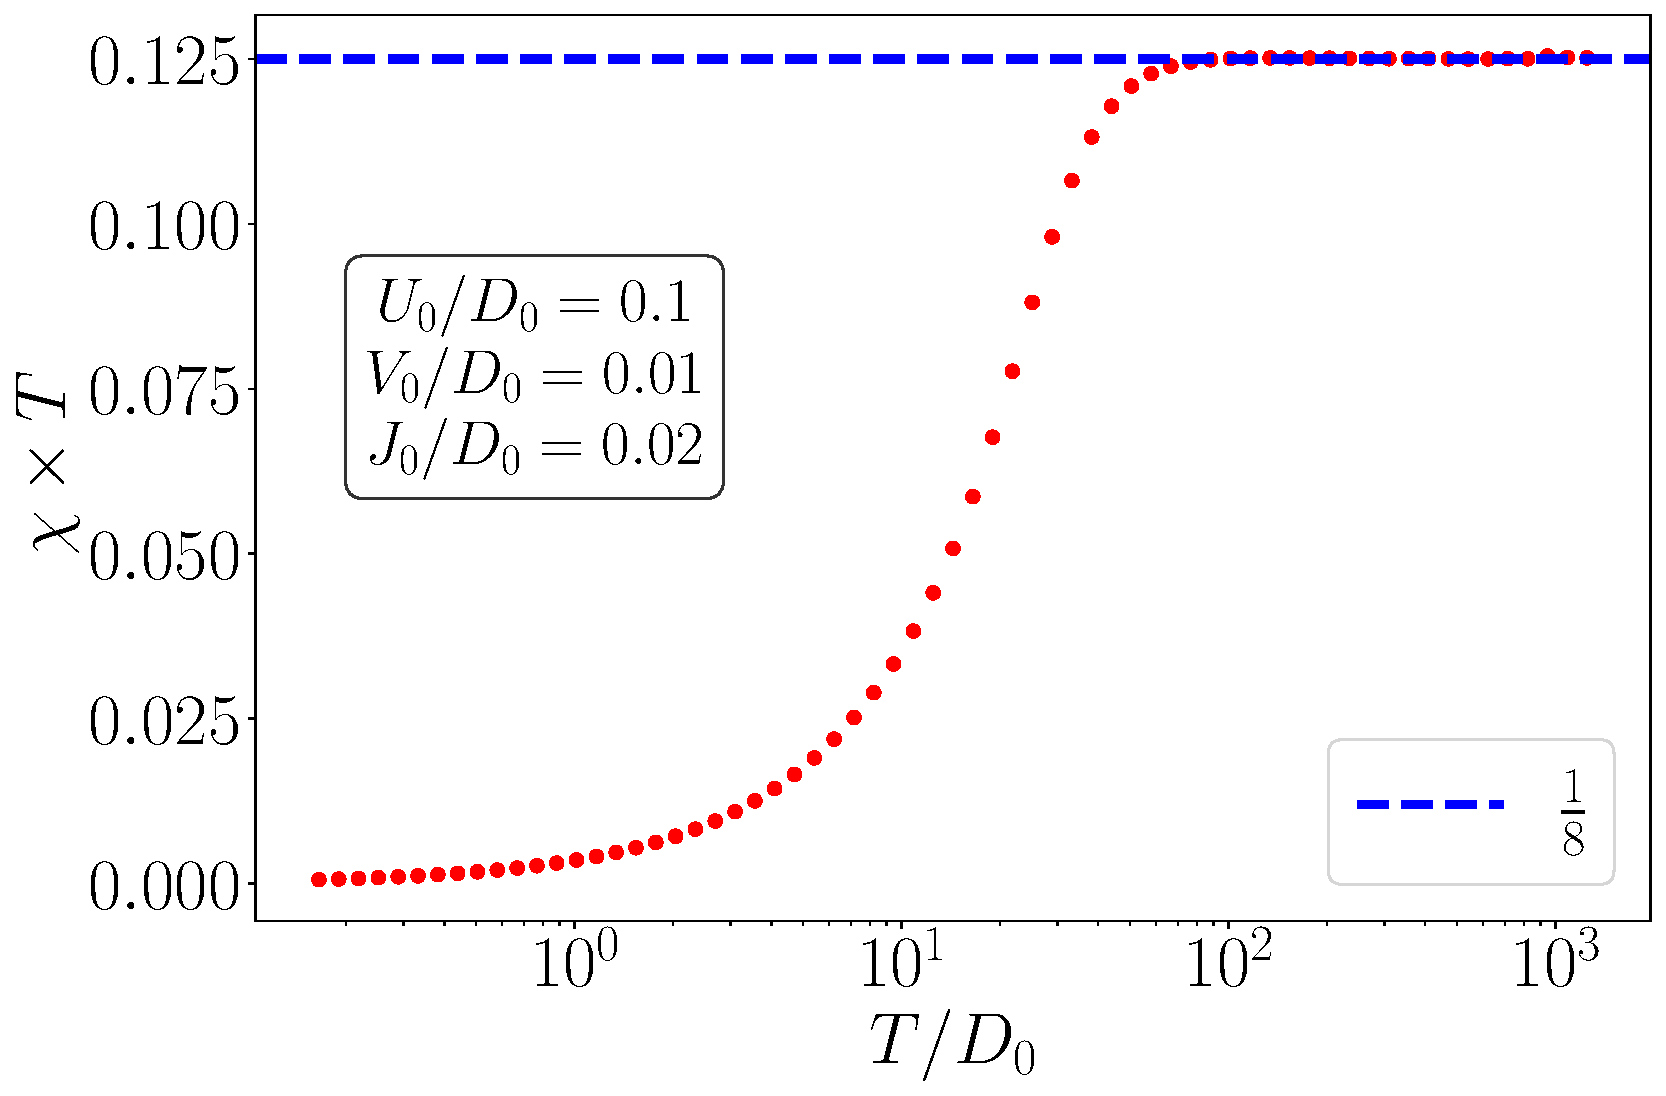
\includegraphics[width=0.49\textwidth]{../figures/chiT_J=0.020.pdf}
	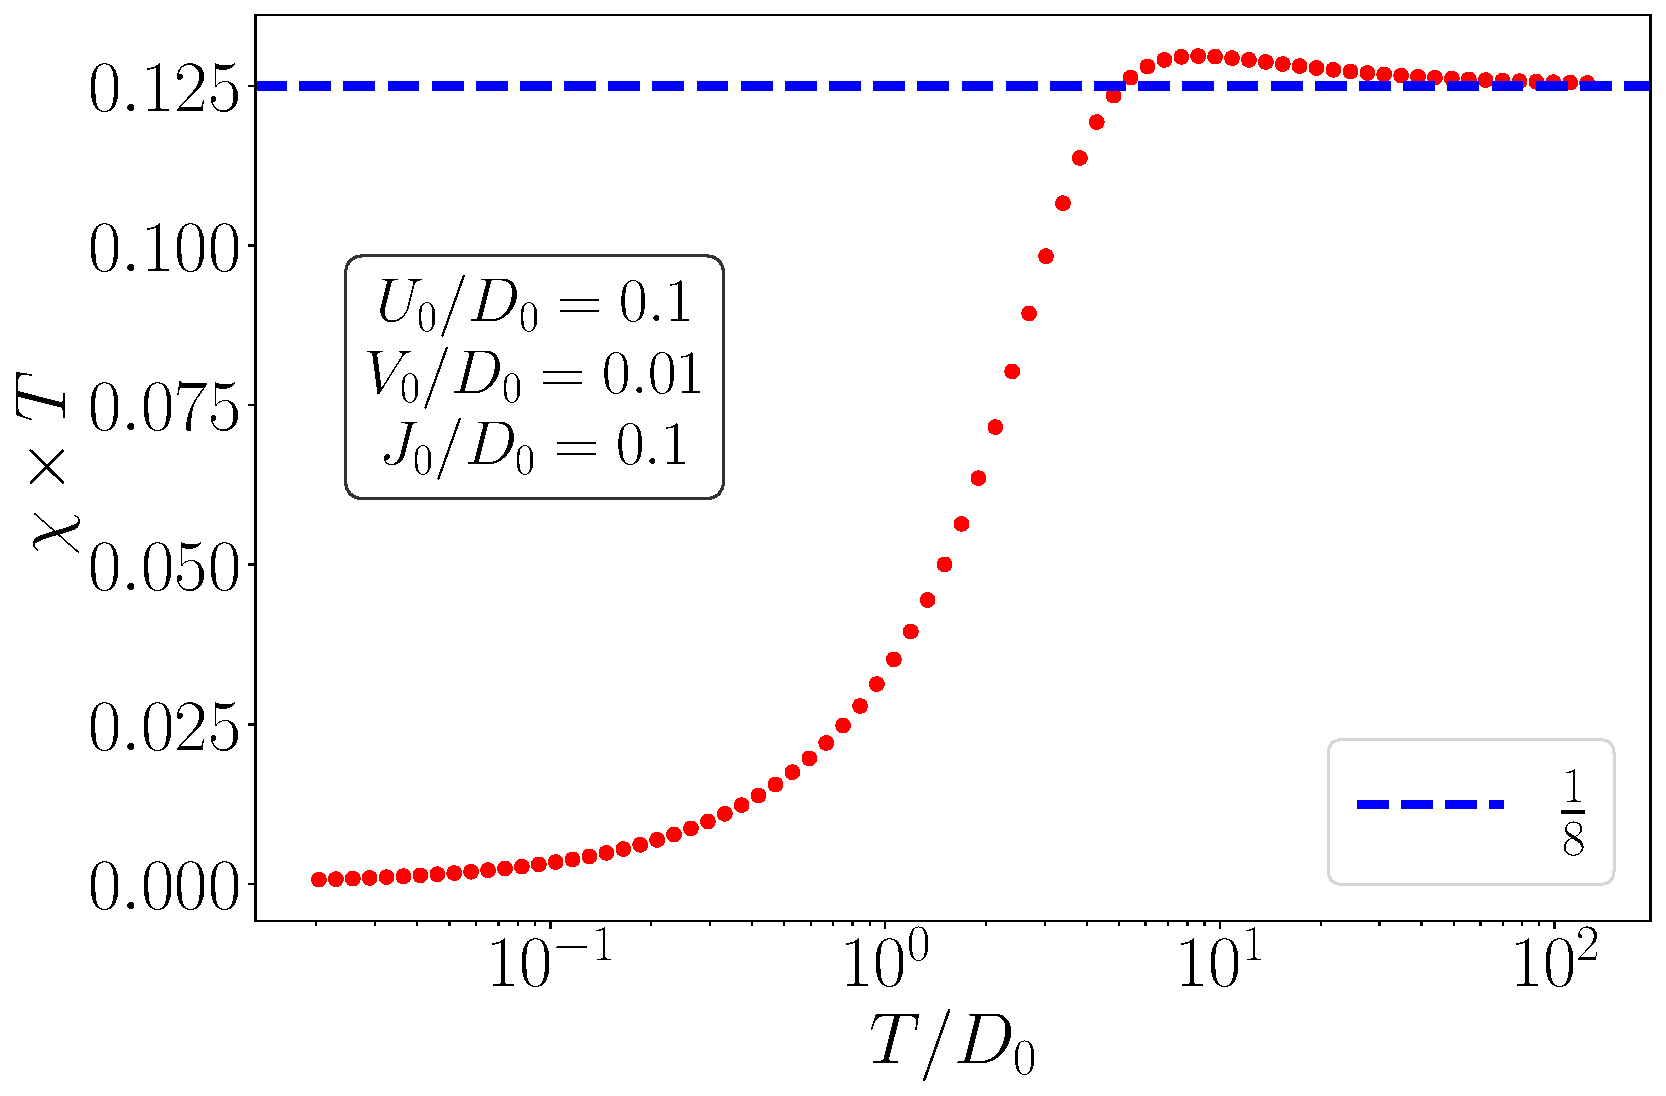
\includegraphics[width=0.49\textwidth]{../figures/chiT_J=0.100.pdf}
	\caption{Spin susceptibility of the impurity times temperature, for two sets of bare parameters, in \(U>0\). At low temperatures, it becomes linear because \(\chi\) itself becomes constant (screening), while at high temperatures, \(\chi\times T\) becomes constant because of the paramagnetic \(\sim 1/T\) form of \(\chi\). For the right panel with a larger value of the spin-exchange coupling, the \(\chi\) tries to go towards the local moment value of \(1/4\) but eventually drops back to the free orbital value of \(1/8\).}
	\label{chi}
\end{figure}

\subsection{Charge susceptibility}
We can similarly define the charge susceptibility as
\begin{equation}\begin{aligned}
	\label{zero_chi_charge}
	\chi(\beta) = \beta \left(\left<\left(C_d^z\right)^2\right> - \left<C_d^z\right>^2\right) = \lim_{B_c \to 0}\frac{1}{\beta}\left[\frac{1}{Z(B_c)} \frac{\partial^2{Z(B_c)}}{\partial{B_c^2}}-\frac{1}{Z(B_c)^2} \left(\frac{\partial{Z(B_c)}}{\partial{B_c}}\right)^2\right]
\end{aligned}\end{equation}
where \(B_c\) is now a field that couples to the impurity charge-isospin:
\begin{equation}\begin{aligned}
	\label{charge_field}
	\mathcal{H}^\prime(B_c) = \mathcal{H} + B_c C_d^z
\end{aligned}\end{equation}
The charge susceptibility for \(U<0\) is shown in fig.~\ref{chi_charge}.
\begin{figure}[htpb]
	\centering
	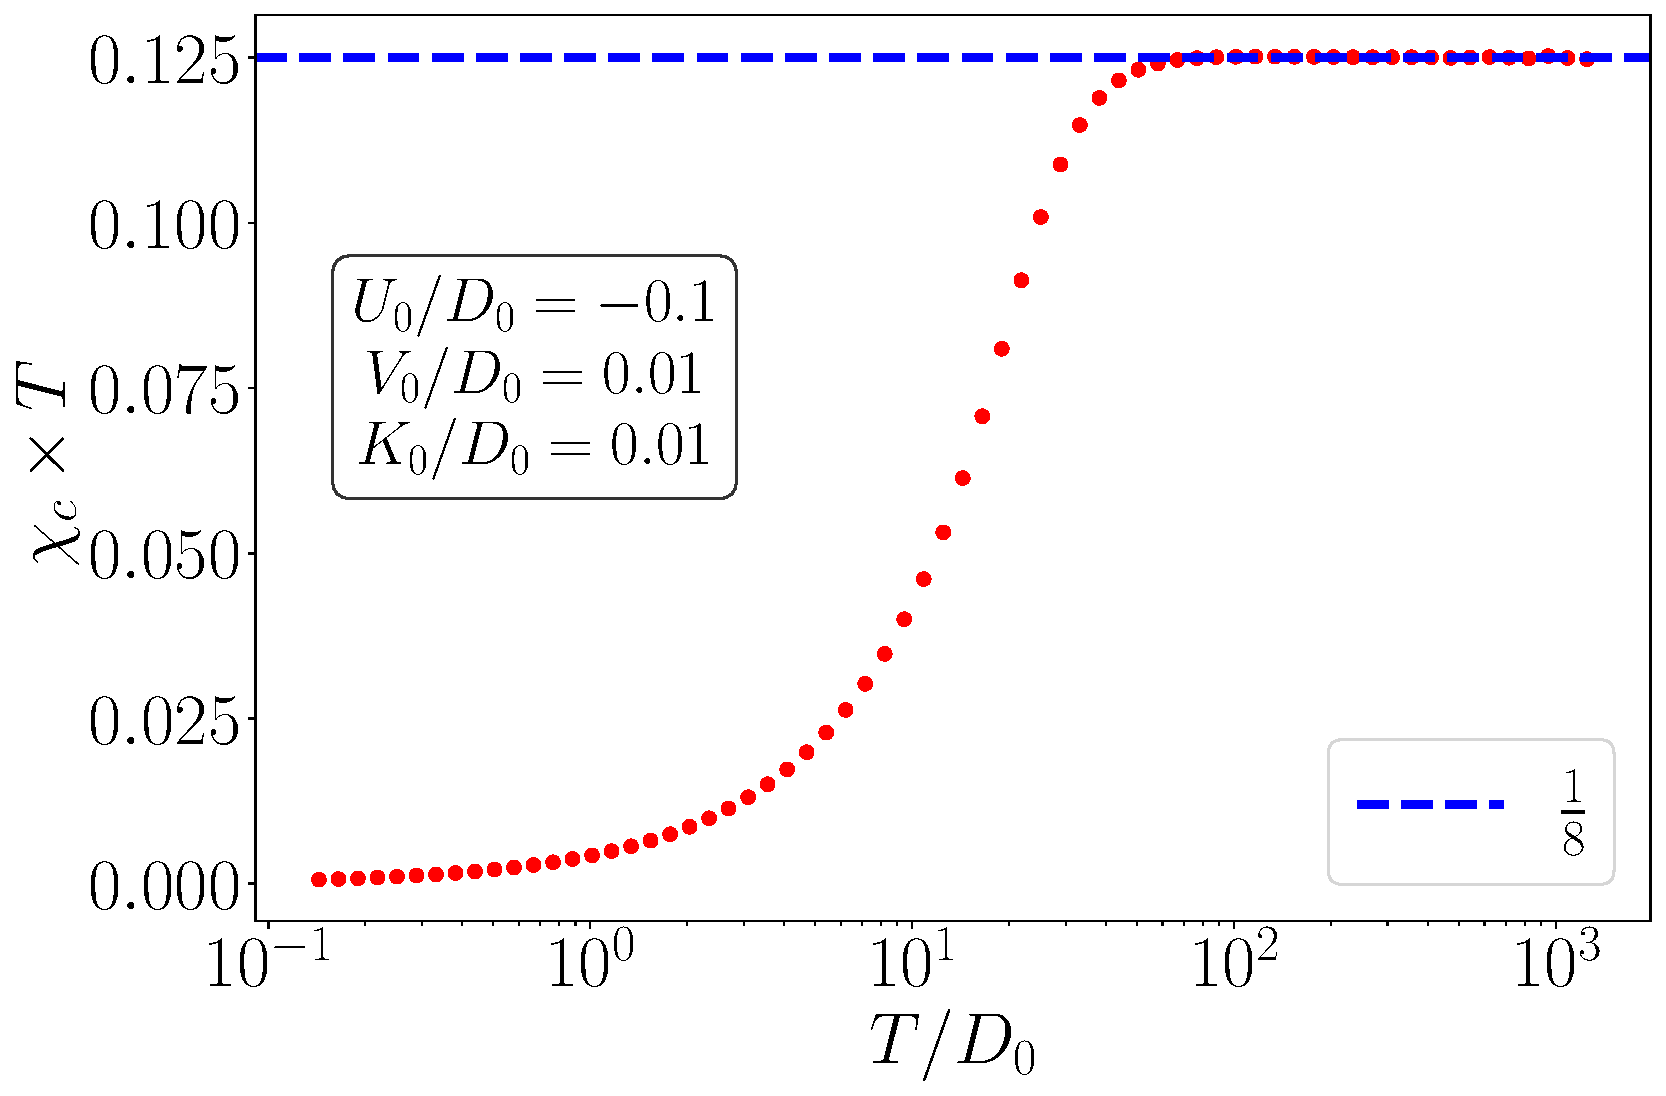
\includegraphics[width=0.49\textwidth]{../figures/chi_chargeT_K=0.010.pdf}
	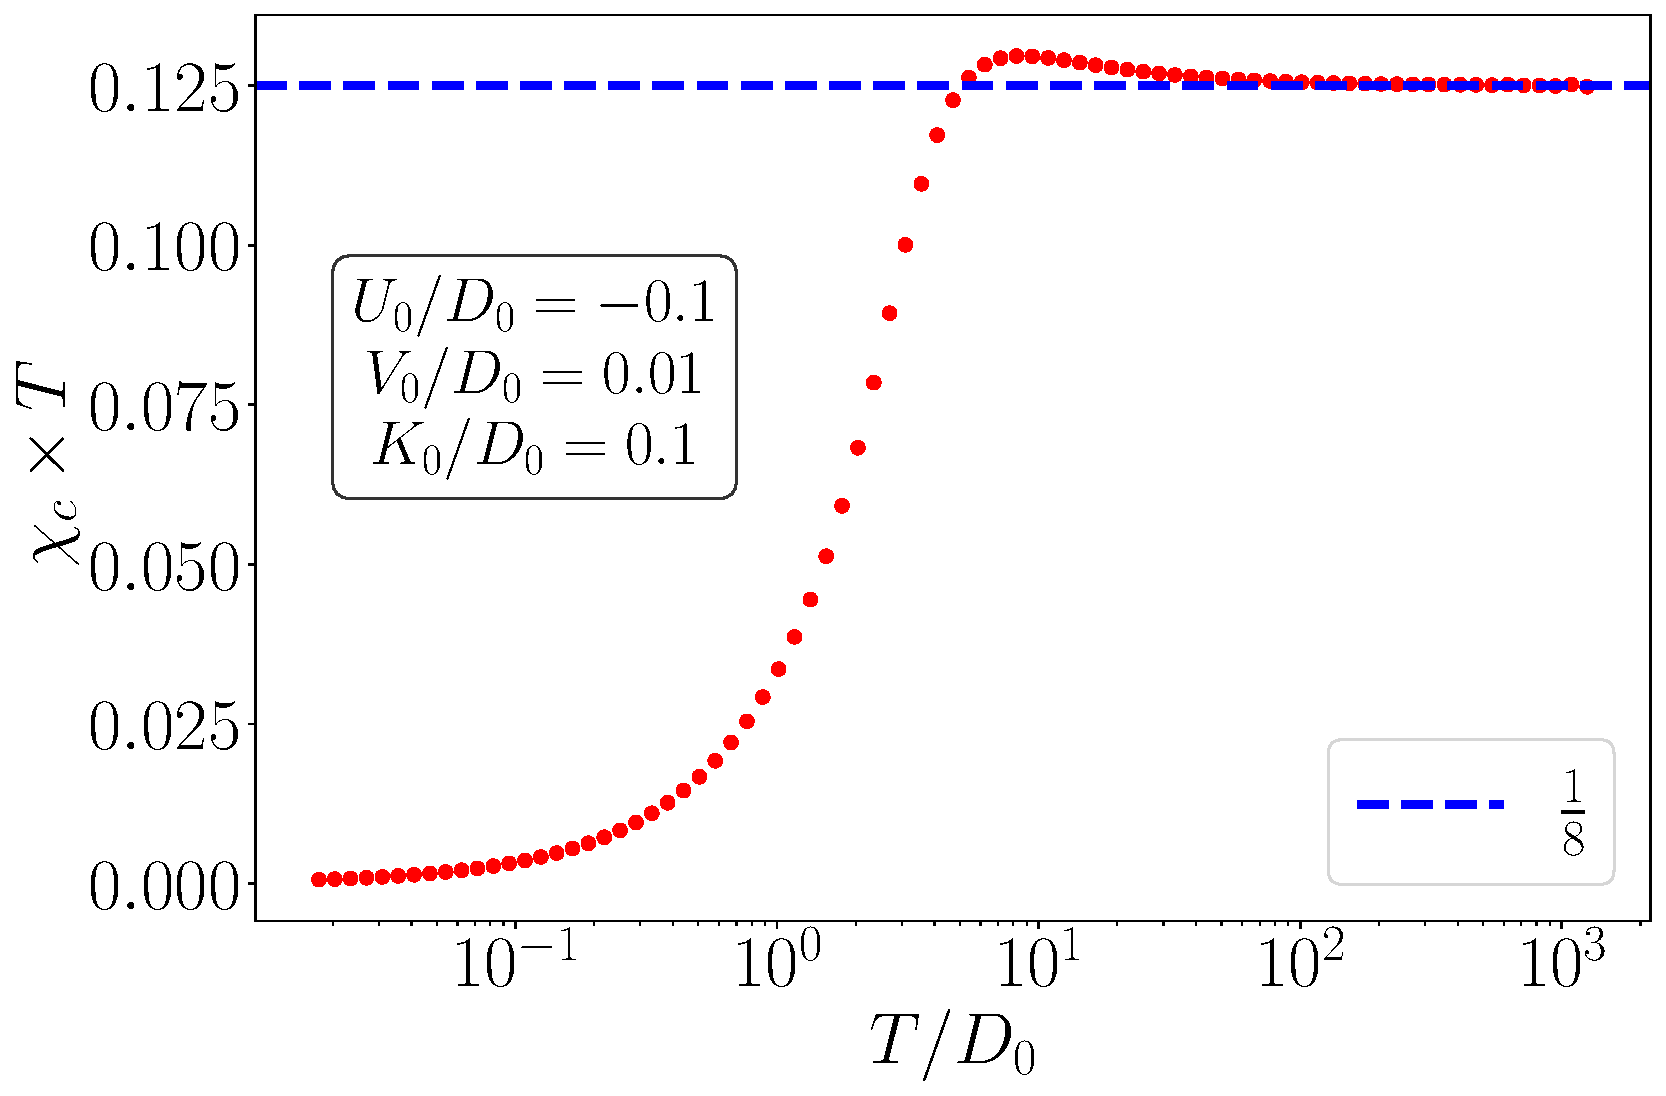
\includegraphics[width=0.49\textwidth]{../figures/chi_chargeT_K=0.100.pdf}
	\caption{Charge susceptibility for the impurity at \(U<0\), for two sets of bare parameters. The physics is very similar to that of the spin susceptibility in \(U>0\).}
	\label{chi_charge}
\end{figure}

It is interesting to look at the behaviour of the charge susceptibility in the positive \(U\) regime, fig.~\ref{chi_charge_posU}. It  is seen that for \(J_0<V_0\), the charge susceptibility is very similar to the spin susceptibility, with a reduced saturation value. This is because, for that range of bare values, the ground state consists of a comparable mixture of the spin and charge states (see fig.~\ref{cs_cc}). This means that the magnetic field term in eq.~\eqref{charge_field} can couple to the charge component of the ground state, and give a non-zero charge susceptibility at zero temperature. On the other hand, for \(J_0 > V_0\), we see that \(\chi_c\) vanishes at low temperatures. This can again be understood from the ground state. For that range of bare values, the ground state can be approximated by purely the singlet, because the charge fraction \(c_-^c\) becomes very small. This means that the field \(B_c \) has nothing to couple with. Alternatively, it can be said that since the ground state has only terms with \(\hat n_d=1\), no number fluctuation is possible, and the impurity isospin is not susceptible at all to charge polarisation.
\begin{figure}[htpb]
	\centering
	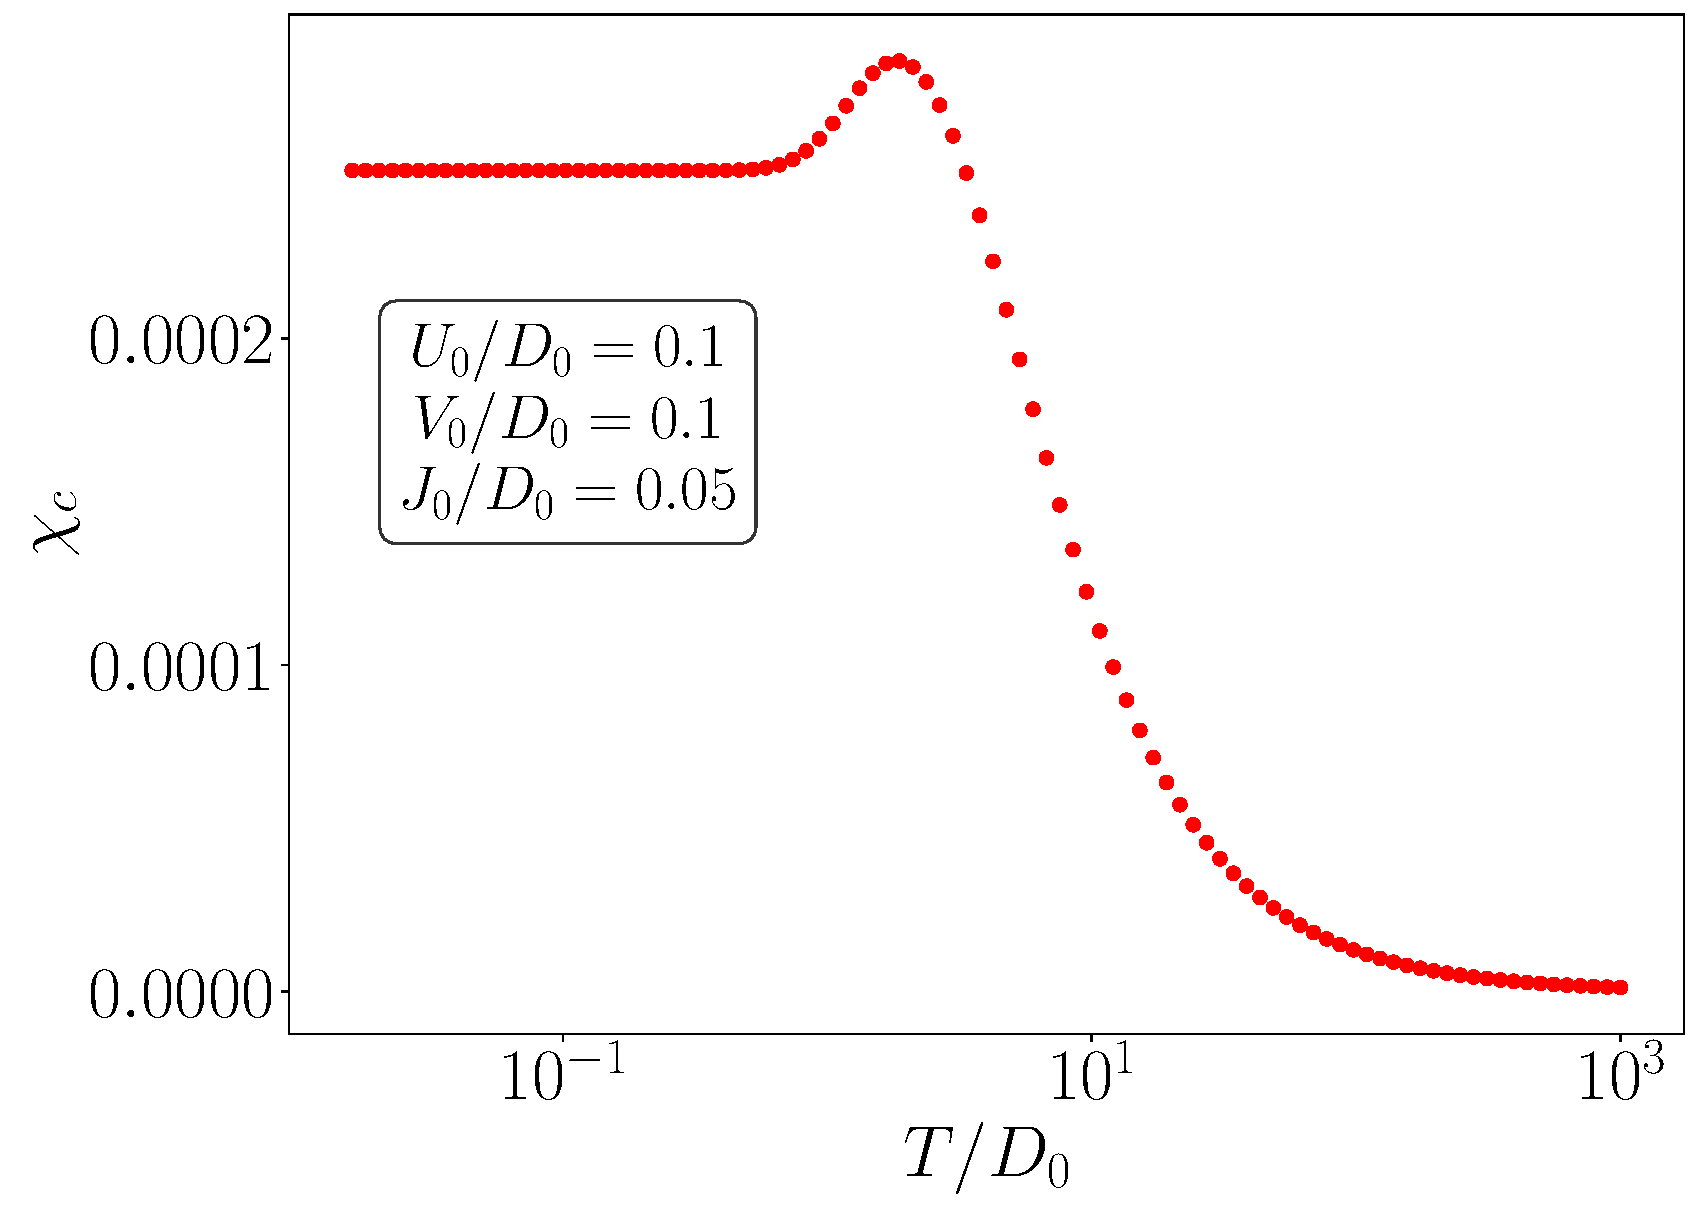
\includegraphics[width=0.48\textwidth]{../figures/chiC_posU_J=small.pdf}
	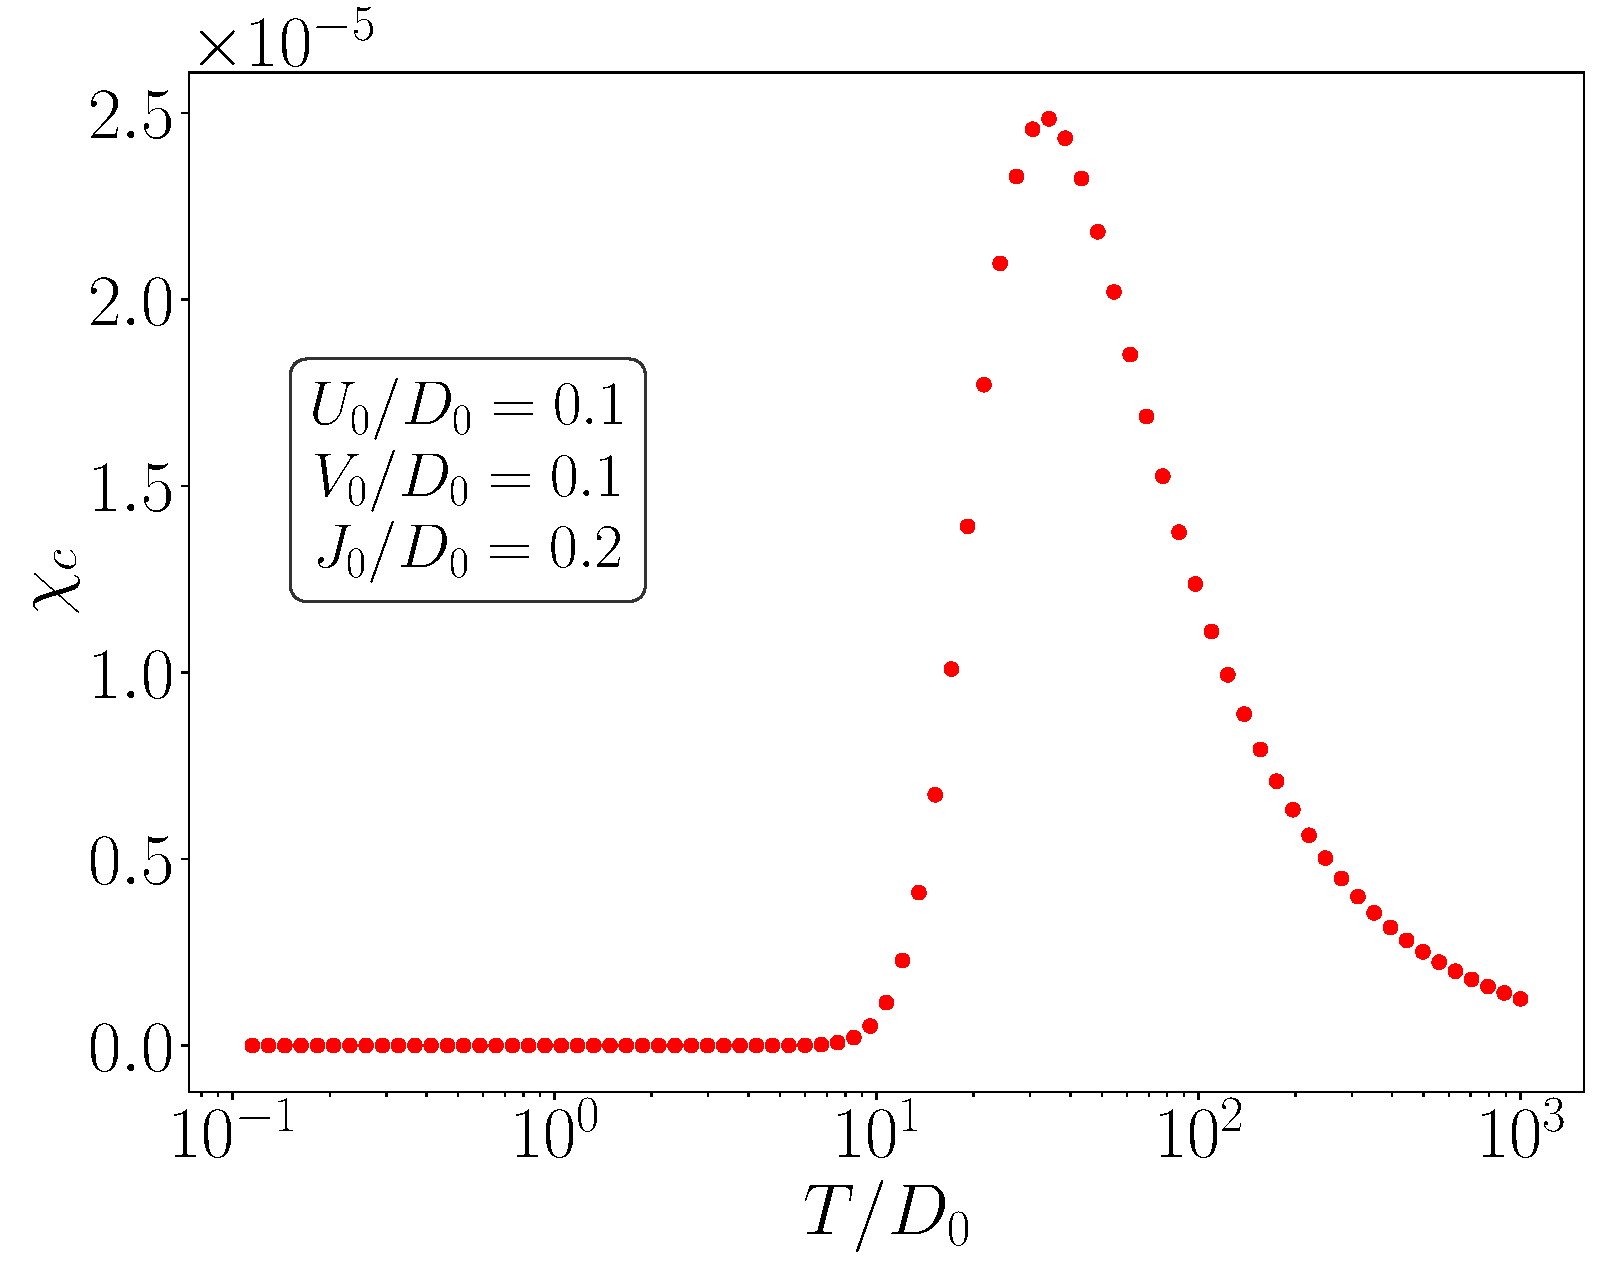
\includegraphics[width=0.48\textwidth]{../figures/chiC_posU_J=large.pdf}
	\caption{Charge susceptibility of the impurity in the positive \(U\) regime, for two values of \(J_0\). The smaller bare value leads to a spin+charge mixed ground state, and hence a non-zero \(\chi_c\) at zero temperature. The larger \(J_0\), however, leads to a purely spin ground state without any number fluctuation, and this gives vanishing \(\chi_c\) at zero temperature.}
	\label{chi_charge_posU}
\end{figure}

From eq.~\eqref{gstate_kondo}, we know that in the thermodynamic limit, the ground state of \(U>0\) regime reduces to a screened local moment. That then implies that the charge susceptibility vanishes at low temperatures, owing to lack of any charge content in the ground state in the large bandwidth limit.
\begin{equation}\begin{aligned}
	\lim_{D_0 \to \infty}\chi_c(U>0, T \to 0) = 0
\end{aligned}\end{equation}

\section{Specific heat}
The specific heat is calculated by diagonalizing the fixed point Hamiltonian, numerically. The obtained spectrum is denoted by \(\left\{ \mathcal{E}_i \right\} \). The total average energy of the impurity+cloud at temperature \(T\) is then
\begin{equation}\begin{aligned}
	\left<\mathcal{E} \right> = \frac{1}{Z}\sum_{i} \mathcal{E}_i e^{-\beta \mathcal{E}_i}
\end{aligned}\end{equation}
where \(Z = \sum_{i} e^{-\beta E_i}\) is the partition function. The specific heat of this system is thus
\begin{equation}\begin{aligned}
	C_V &= \frac{\partial{\left<\mathcal{E} \right>}}{\partial{T}} \\
	    &= -\frac{1}{k_B T^2} \frac{\partial{\left<\mathcal{E} \right>}}{\partial{\beta}} \\
	    &= \frac{1}{k_B T^2}\left[\frac{1}{Z}\sum_i \mathcal{E}_i^2 e^{-\beta \mathcal{E}_i} - \left(\frac{1}{Z}\sum_i \mathcal{E}_i e^{-\beta \mathcal{E}_i}\right)^2 \right] 
\end{aligned}\end{equation}
In the absence of impurity, the eigenvalues of the Hamiltonian are \(\left\{\mathcal{E}_i^0\right\}\) with a partition function \(Z^0 = \sum_{i} e^{-\beta E_i^0}\), so the bath specific heat is
\begin{equation}\begin{aligned}
	C_V^0 &= \frac{1}{k_B T^2}\left[\frac{1}{Z_0}\sum_i \mathcal{E}_i^2 e^{-\beta \mathcal{E}_i^0} - \left(\frac{1}{Z_0}\sum_i \mathcal{E}_i^0 e^{-\beta \mathcal{E}_i^0}\right)^2 \right] 
\end{aligned}\end{equation}
The impurity specific heat is the difference.
\begin{equation}\begin{aligned}
	C_V^\text{imp} = C_V - C_V^0
\end{aligned}\end{equation}
These values were calculated numerically and plotted against temperature in fig.~\ref{cv}.
\begin{figure}[htpb]
	\centering
	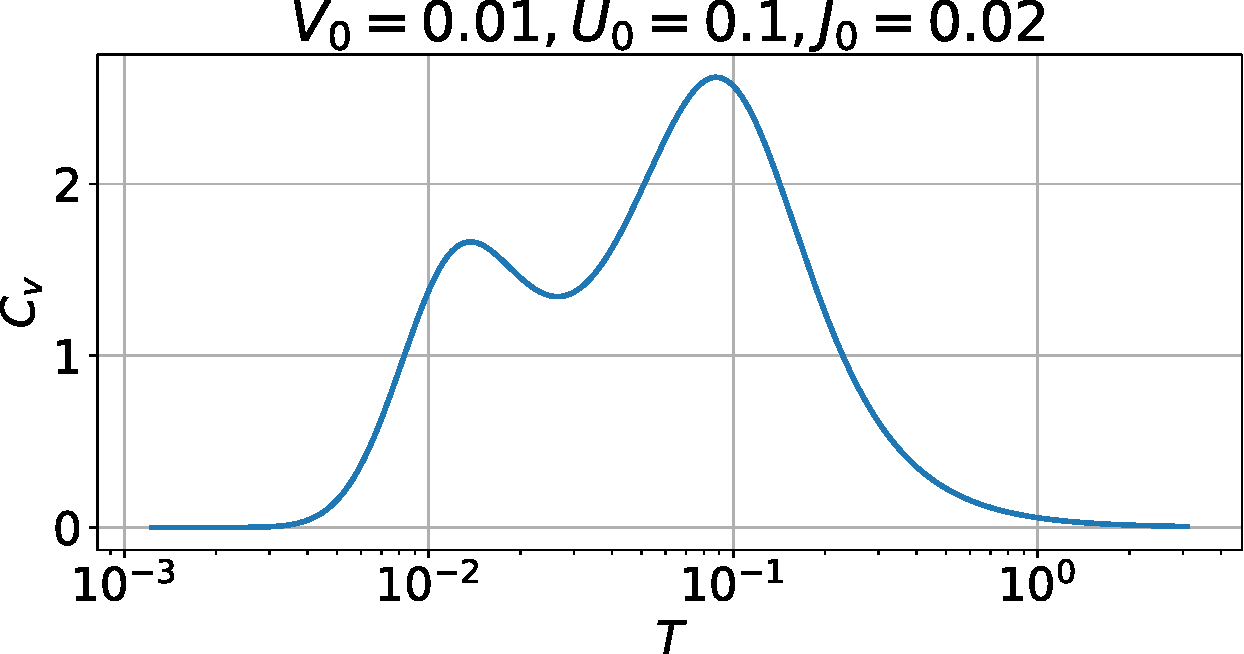
\includegraphics[width=0.6\textwidth]{../figures/Cv.pdf}
	\caption{Impurity specific heat}
	\label{cv}
\end{figure}

\section{Renormalization of impurity spectral function}
In this section we will obtain the impurity spectral function, which is defined in terms of the impurity Green's function as
\begin{equation}\begin{aligned}
	\mathcal{A(\omega)} = -\frac{1}{\pi}\text{ Im }\left[G_{dd}^\sigma\left( \omega \right) \right] 
\end{aligned}\end{equation}
The impurity retarded Green's function (assuming the Hamiltonian to be time-independent, which it is) is defined as
\begin{equation}\begin{aligned}
	G_{dd}^\sigma(t) = -i\theta(t) \left<\left\{ c_{d\sigma}(t),c^\dagger_{d\sigma} \right\}  \right>
\end{aligned}\end{equation}
where the average \(\left< \right>\) is over a canonical ensemble at temperature \(T\). What follows is a standard calculation where we write the Green's function in the Lehmann representation. We will write the ensemble average in terms of the exact eigenstates of the fixed point Hamiltonian:
\begin{equation}\begin{aligned}
	H^* \ket{n} &= E_n^* \ket{n}\\
	\left<\hat O \right> &\equiv \frac{1}{Z}\sum_n \bra{n} \hat O \ket{n} e^{-\beta E_n^*}
\end{aligned}\end{equation}
where \(Z = \sum_n e^{-\beta E_n^*}\) is the fixed point partition function and \(\left\{ \ket{n} \right\} \) is the set of eigenfunctions of the fixed point Hamiltonian. We can therefore write
\begin{equation}\begin{aligned}
	&\left<\left\{ c_{d\sigma}(t),c^\dagger_{d\sigma} \right\}  \right> \\
	&= \frac{1}{Z}\sum_{m}e^{-\beta E_m}\bra{m}\left\{ c_{d\sigma}(t),c^\dagger_{d\sigma} \right\} \ket{m}\\
	&= \frac{1}{Z}\sum_{m,n}e^{-\beta E_m}\bra{m}\left( c_{d\sigma}(t)\ket{n}\bra{n}c^\dagger_{d\sigma} + c^\dagger_{d\sigma}\ket{n}\bra{n}c_{d\sigma}(t)\right) \ket{m} && \left[\sum_n \ket{n}\bra{n} = 1\right]  \\
	&= \frac{1}{Z}\sum_{m,n}e^{-\beta E_m}\bra{m}\left( e^{iH^* t}c_{d\sigma}e^{-iH^* t}\ket{n}\bra{n}c^\dagger_{d\sigma} + c^\dagger_{d\sigma}\ket{n}\bra{n}e^{iH^* t}c_{d\sigma}e^{-iH^* t}\right) \ket{m}\\
	&= \frac{1}{Z}\sum_{m,n}e^{-\beta E_m}\left( e^{i\left( E_m - E_n \right)  t}\bra{m}c_{d\sigma}\ket{n}\bra{n}c^\dagger_{d\sigma} \ket{m} + e^{i\left( E_n - E_m \right)  t}\bra{m}c^\dagger_{d\sigma}\ket{n}\bra{n}c_{d\sigma} \ket{m}\right)\\
	&= \frac{1}{Z}\sum_{m,n}e^{i\left( E_m - E_n \right)  t}||\bra{m}c_{d\sigma}\ket{n}||^2\left( e^{-\beta E_m} + e^{-\beta E_n}\right)\\
\end{aligned}\end{equation}
The time-domain impurity Green's function can thus be written as (this is the so-called Lehmann representation)
\begin{equation}\begin{aligned}
	G_{dd}^\sigma = -i\theta(t)\frac{1}{Z}\sum_{m,n}e^{i\left( E_m - E_n \right)  t}||\bra{m}c_{d\sigma}\ket{n}||^2\left( e^{-\beta E_m} + e^{-\beta E_n}\right)\\
\end{aligned}\end{equation}
We are interested in the frequency domain form.
\begin{equation}\begin{aligned}
	G_{d d}^\sigma(\omega) &= \int_{-\infty}^\infty dt e^{i \omega t}G_{d d}^\sigma(t) \\
			       &= \frac{1}{Z}\sum_{m,n}||\bra{m}c_{d\sigma}\ket{n}||^2\left( e^{-\beta E_m} + e^{-\beta E_n}\right)\left(-i\right)\int_{-\infty}^\infty dt \theta(t)e^{i\left( \omega + E_m - E_n \right)t}
\end{aligned}\end{equation}
To evaluate the time-integral, we will use the integral representation of the Heaviside function:
\begin{equation}\begin{aligned}
	\theta(t) = \frac{1}{2\pi i}\lim_{\eta \to 0^+} \int_{-\infty}^\infty \frac{1}{x- i\eta}e^{ixt}dx
\end{aligned}\end{equation}
With this definition, the integral in \(G_{dd}^\sigma(\omega)\) becomes
\begin{equation}\begin{aligned}
	\left(-i\right)\int_{-\infty}^\infty dt \theta(t)e^{i\left( \omega + E_m - E_n \right)t} &= \left(-i\right)\frac{1}{2\pi i}\lim_{\eta \to 0^+} \int_{-\infty}^\infty dx\frac{1}{x- i\eta}\int_{-\infty}^\infty dt e^{i\left( \omega + E_m - E_n + x\right)t} \\
									     &=\left(-i\right)\frac{1}{2\pi i}\lim_{\eta \to 0^+} \int_{-\infty}^\infty dx\frac{1}{x- i\eta} 2\pi \delta\left( \omega + E_m - E_n + x\right) \\
									     &=\left(-i\right)\frac{1}{i}\lim_{\eta \to 0^+} \frac{-1}{\omega + E_m - E_n- i\eta} \\
									     &=\frac{1}{\omega + E_m - E_n} \\
\end{aligned}\end{equation}
The frequency-domain Green's function is thus
\begin{equation}\begin{aligned}
	G_{d d}^\sigma(\omega) = \frac{1}{Z}\sum_{m,n}||\bra{m}c_{d\sigma}\ket{n}||^2\left( e^{-\beta E_m} + e^{-\beta E_n}\right)\frac{1}{\omega + E_m - E_n}
\end{aligned}\end{equation}
The zero temperature Green's function is obtained by taking the limit of \(\beta \to \infty\). In both the partition function as well as inside the summation, the only term that will survive is the exponential of the ground state energy \(E_0\).
\begin{equation*}\begin{aligned}
	Z \equiv \sum_m e^{-\beta E_m} \implies \lim_{\beta \to \infty}Z = d_0 e^{-\beta E_0}, && E_0 \equiv \text{min}\left\{ E_n \right\} 
\end{aligned}\end{equation*}
where \(d_0\) is the degeneracy of the ground state. The Greens function then simplifies to
\begin{equation}\begin{aligned}
	G_{d d}^\sigma(\omega, \beta \to \infty) &= \frac{1}{d_0e^{-\beta E_0}}\sum_{m,n}||\bra{m}c_{d\sigma}\ket{n}||^2\left[e^{-\beta E_m}\delta_{E_m, E_0} + e^{-\beta E_n}\delta_{E_n, E_0}\right]\frac{1}{\omega + E_m - E_n}\\
						 &= \frac{1}{d_0}\sum_{n,0}\left[||\bra{0}c_{d\sigma}\ket{n}||^2\frac{1}{\omega + E_0 - E_n} + ||\bra{n}c_{d\sigma}\ket{0}||^2\frac{1}{\omega - E_0 + E_n}\right]\\
\end{aligned}\end{equation}
The label 0 sums over all states \(\ket{0}\) with energy \(E_0\). The spectral function is the imaginary part of this Green's function. To extract the imaginary part, we insert an infinitesimal imaginary part in the denominator:
\begin{equation}\begin{aligned}
	G_{d d}^\sigma(\omega, \eta) = \frac{1}{d_0}\lim_{\eta \to 0^-}\sum_{n,0}\left[||\bra{0}c_{d\sigma}\ket{n}||^2\frac{1}{\omega + E_0 - E_n + i\eta} + ||\bra{n}c_{d\sigma}\ket{0}||^2\frac{1}{\omega - E_0 + E_n + i\eta}\right]\\
\end{aligned}\end{equation}
The spectral function at zero temperature can then be written as
\begin{equation}\begin{aligned}
	\mathcal{A(\omega)} &= -\frac{1}{\pi}\text{ Im }\left[G_{dd}^\sigma\left( \omega \right) \right] \\
			    &= \frac{1}{d_0}\frac{1}{\pi}\text{ Im }\left[\lim_{\eta \to 0^-}\sum_{n,0}\left(\frac{-i\eta ||\bra{0}c_{d\sigma}\ket{n}||^2}{\left(\omega + E_0 - E_n\right)^2 + \eta^2} + \frac{-i\eta ||\bra{n}c_{d\sigma}\ket{0}||^2}{\left(\omega - E_0 + E_n\right)^2 + \eta^2}\right)\right]\\
			    &= \frac{1}{d_0}\frac{1}{\pi}\sum_{n,0}\left[||\bra{0}c_{d\sigma}\ket{n}||^2\pi\delta\left(\omega + E_0 - E_n\right) + ||\bra{n}c_{d\sigma}\ket{0}||^2\pi\delta\left(\omega - E_0 + E_n\right)\right]\\
			    &= \frac{1}{d_0}\sum_{n,0}\left[||\bra{0}c_{d\sigma}\ket{n}||^2\delta\left(\omega + E_0 - E_n\right) + ||\bra{n}c_{d\sigma}\ket{0}||^2\delta\left(\omega - E_0 + E_n\right)\right]\\
\end{aligned}\end{equation}
Since this is in terms of the exact eigenstates, it is a discrete sum of delta-functions. In practice, we get a continuous distribution. To compare with experiment, we need to convert the discrete sum into a continuous function. Following \cite{bullaNRGreview}, we replace the delta-functions at \(\pm x_n \equiv \pm(E_n - E_0)\) by normalized Gaussian functions
\begin{equation}\begin{aligned}
	\delta(\omega \pm x_n) \to \frac{1}{\eta_n\sqrt \pi}e^{-\left(\frac{\omega \pm x_n}{\eta_n}\right)^2}
\end{aligned}\end{equation}
The parameter \(\eta_n\) determines the height and width of the Gaussian, and is chosen such that the higher energy poles are broader than the lower energy ones:
\begin{equation}\begin{aligned}
	\eta_n = 4\Delta + \frac{1}{2}|x_n| 
\end{aligned}\end{equation}
\(\Delta = \pi \rho(0)V^2\) is the relevant energy scale for the non-interacting \((U=0)\) problem, \(\rho(0)\) being the density of states of the conduction bath at the Fermi energy. As a result, the function that we will numerically compute and plot is
\begin{equation}\begin{aligned}
	\mathcal{A(\omega)} &= \sum_{n,0}\frac{1}{d_0 \sqrt \pi \eta_n}\left[||\bra{0}c_{d\sigma}\ket{n}||^2e^{-\left(\frac{\omega - x_n}{\eta_n}\right)^2} + ||\bra{n}c_{d\sigma}\ket{0}||^2e^{-\left(\frac{\omega + x_n}{\eta_n}\right)^2}\right]
\end{aligned}\end{equation}
From the results of Langreth \cite{langreth1966}, we know that the spectral function at zero frequency is fixed by the occupancy of the impurity. Since we are in the particle-hole symmetric regime, this occupancy is fixed at 1, and hence so is the spectral function height at \(\omega = 0\). This result has been used to fix the spectral function height at the center during the computations. The fixed-point Hamiltonian \(H^*\) is diagonalized numerically to obtain \(\left\{E_n, \ket{n}\right\}\), for various values of the couplings. The intention here is to get an idea of how the spectral function morphs under the RG. Doing an actual reverse RG (described in \ref{rev_rg}) would require us to diagonalize a huge Hamiltonian. We take the simpler route of tuning the \(U\) from zero to soem large value. This should mimic the journey from the IR theory \((U=0)\) to the UV theory \((U \gg 0)\).

The spectral function is plotted for three sets of values in fig.~\ref{spec_func}. For low values of \(U\), the profile is that of a single peak at zero frequency. This is expected because at the low energy effective theory, the high energy Hubbard side bands have been integrated out. As \(U\) increases, shoulder-like structures appear on either side of the peak, which finally, at larger \(U\), develop into two side-peaks. This is the microscopic theory, where high energy features are also relevant.
\begin{center}
	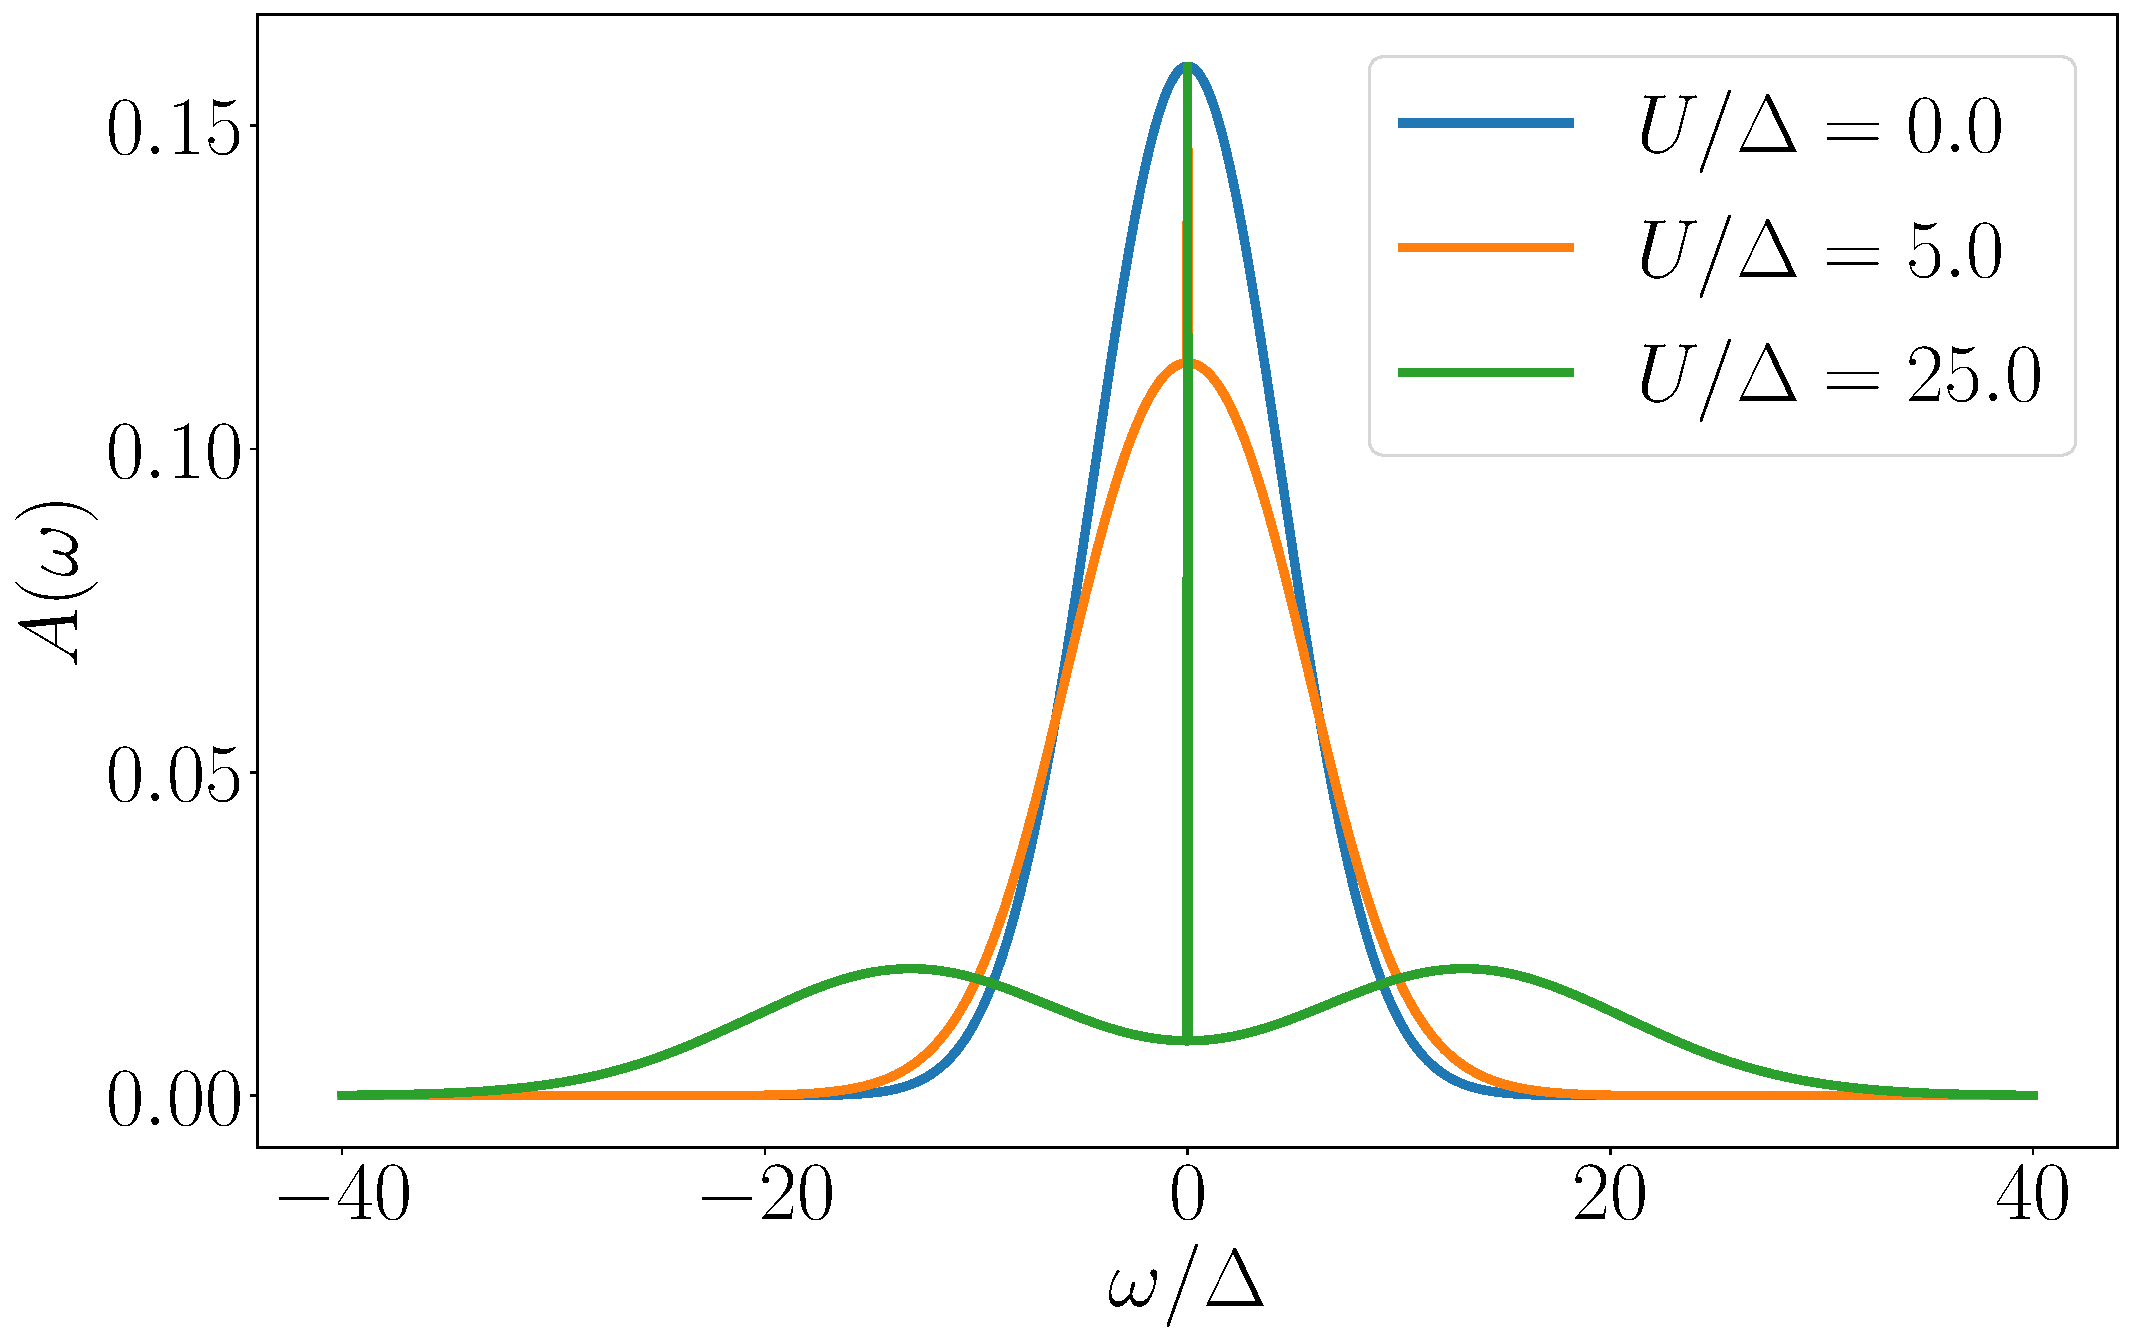
\includegraphics[width=0.8\textwidth]{../figures/gen_siam_spec_func.pdf}
	\captionof{figure}{Impurity spectral function for multiple values of \(U\). The increase in value of \(U\) is accompanied by the appearance of the side-peaks.}
	\label{spec_func}
\end{center}
The physics of the three peaks can now be looked into. Since the central peak is at zero energy, it has to do with excitations that do not cost any energy. There are two such excitations: excitations within the spin sector and within the charge sector.
\begin{equation}\begin{aligned}
	\ket{\uparrow} \mathrel{\mathlarger{\mathlarger{\mathop{\rightleftarrows}}^{J S_d^-}_{JS_d^+}}}\ket{\downarrow}, &&&&\ket{\Uparrow} \mathrel{\mathlarger{\mathlarger{\mathop{\rightleftarrows}}^{K C_d^-}_{K C_d^+}}}\ket{\Downarrow}\\
\end{aligned}\end{equation}
The thick arrow \(\Uparrow\) represents the charge isospin. At particle-hole symmetry, both the spin configurations has energy of \(\epsilon_d\), while the charge configurations have energy of \(2\epsilon_d + U=0\) and 0. Hence, no energy is required for these excitations, which is why see a macroscopic number of cloud electrons resonating with the impurity at the Fermi surface. Also note that if \(\hat S_i\) and \(\hat C_j\) are two operators of the spin and charge sector (\(i,j \in \left\{ x,y,z \right\} \)), then
\begin{equation}\begin{aligned}
	\hat S_i \hat C_j = \hat C_j \hat S_i = 0
\end{aligned}\end{equation}
We can see this by applying that operator on a basis state. Since the set of four states 
\begin{equation}\begin{aligned}
	\ket{\hat S_i = \pm \frac{1}{2}, \hat C_j = 0}, \ket{\hat S_i = 0, \hat C_j = \pm\frac{1}{2}}
\end{aligned}\end{equation}
are all independent, they form a basis. If we apply the operator on these states:
\begin{equation}\begin{aligned}
	\hat S_i \hat C_j \ket{\hat S_i} &= 0, &&&&\hat C_j \hat S_i \ket{S_i} = S_i \hat C_j \ket{S_i} = 0\\
	\hat C_j \hat S_i \ket{C_j} &= 0, &&&&\hat S_i \hat C_j \ket{\hat C_j} = C_j \hat S_i \ket{\hat C_j} = 0 \\
\end{aligned}\end{equation}
This shows that each operator acts only on its own subspace. \(S_i\) does not act on the charge sector, and vice-versa. There is no single-particle excitation here.

The physics of the side-peaks is that of single number fluctuations on the impurity. These are brought about by the term \(Vc^\dagger_{0\sigma}c_{d\sigma} + \text{h.c.}\).
\begin{equation}\begin{aligned}
	\left( \epsilon_d  \right) \ket{\sigma} & \mathrel{\mathlarger{\mathlarger{\mathop{\rightleftarrows}}^{V c^\dagger_{d\overline\sigma}/V c_{d\sigma}}_{V c_{d\overline\sigma}/V c^\dagger_{d\sigma}}}} &\ket{n_d=2,0} \left( 0 \right) \\
\end{aligned}\end{equation}
These transitions involve energy transfer of the order of \(\epsilon_d\). This is why, at very small \(U\), they remain absorbed inside the central peak. These transitions do not involve any spin or charge-flip, rather they take the impurity between the spin and charge sectors.

\section{Effective Hamiltonian for excitations of the Kondo cloud}
To find an effective Hamiltonian for the excitations of the Kondo cloud, we will integrate out the impurity part of the wavefunction. The Schrodinger equation for the \(J > K\) ground state is
\begin{equation}\begin{aligned}
	E_g &\left[c_-^s \left(\ket{\uparrow, \downarrow} - \ket{\downarrow, \uparrow}\right) + c^c_- \left(\ket{\uparrow\downarrow, 0} + \ket{0, \uparrow\downarrow}\right)\right] \\
	    &= \mathcal{H} \left[c_-^s \left(\ket{\uparrow, \downarrow} - \ket{\downarrow, \uparrow}\right) + c^c_- \left(\ket{\uparrow\downarrow, 0} + \ket{0, \uparrow\downarrow}\right)\right]\\
	    &= \mathcal{H}_0^* \left[c_-^s \left(\ket{\uparrow, \downarrow} - \ket{\downarrow, \uparrow}\right) + c^c_- \left(\ket{\uparrow\downarrow, 0} + \ket{0, \uparrow\downarrow}\right)\right]\\
	    &+V\sum_{\beta}\left[c^\dagger_{2\beta}c_{1\beta} - c_{2\beta}c^\dagger_{1\beta}\right]\left[c_-^s \left(\ket{\uparrow, \downarrow} - \ket{\downarrow, \uparrow}\right) + c^c_- \left(\ket{\uparrow\downarrow, 0} + \ket{0, \uparrow\downarrow}\right)\right]\\
	    &+ J \vec{S_d}\cdot\vec{s}\left[c_-^s \left(\ket{\uparrow, \downarrow} - \ket{\downarrow, \uparrow}\right) + c^c_- \left(\ket{\uparrow\downarrow, 0} + \ket{0, \uparrow\downarrow}\right)\right]\\
	    &+ K \vec{C_d}\cdot\vec{c}\left[c_-^s \left(\ket{\uparrow, \downarrow} - \ket{\downarrow, \uparrow}\right) + c^c_- \left(\ket{\uparrow\downarrow, 0} + \ket{0, \uparrow\downarrow}\right)\right]
\end{aligned}\end{equation}
The last two lines gives
\begin{equation}\begin{aligned}
\frac{1}{2}Jc_-^s \left[s^z \left(\ket{\uparrow, \downarrow} + \ket{\downarrow, \uparrow}\right) +  s^+ \ket{\downarrow, \downarrow} - s^-\ket{\uparrow, \uparrow}\right] + \frac{1}{2}Kc^c_- \left[c^z\left(\ket{\uparrow\downarrow, 0} - \ket{0, \uparrow\downarrow}\right) + c^+\ket{0, 0} \right.\\
+ \left.c^-\ket{2, 2}\right]
\end{aligned}\end{equation}
The second line gives
\begin{equation}\begin{aligned}
	V c^\dagger_{2\uparrow}\left[c_-^s \left(\ket{0, \downarrow}\right) + c^c_- \left(\ket{\downarrow, 0}\right)\right] + V c^\dagger_{2 \downarrow}\left[c_-^s \left(- \ket{0, \uparrow}\right) + c^c_- \left(\ket{\uparrow, 0}\right)\right] \\
	- Vc_{2 \uparrow}\left[c_-^s \left(- \ket{ \uparrow\downarrow, \uparrow}\right) + c^c_- \left(\ket{\uparrow, \uparrow\downarrow}\right)\right] - V c_{2 \downarrow}\left[c_-^s \left(-\ket{ \uparrow\downarrow, \downarrow}\right) + c^c_- \left(\ket{ \downarrow, \uparrow\downarrow}\right)\right]
\end{aligned}\end{equation}
We will now write down four equations by comparing the coefficients of \(\ket{ \uparrow}, \ket{ \downarrow}, \ket{0}\) and \(\ket{2}\) of the impurity sector:
\begin{equation}\begin{aligned}
	\left( E_g - H_0^* \right) c_-^s \ket{\downarrow} &= V c^c_- \left( c^\dagger_{2 \downarrow}\ket{0} - c_{2 \uparrow}\ket{2} \right) + \frac{1}{2}J c^s_-\left( s^z\ket{ \downarrow} - s^-\ket{\uparrow} \right) && \left[\text{eq. from }\ket{\uparrow}\right] \\
	\left( -E_g + H_0^* \right) c_-^s \ket{\uparrow} &= V c^c_- \left( c^\dagger_{2 \uparrow}\ket{0} - c^\dagger_{2 \downarrow}\ket{2} \right) + \frac{1}{2}J c^s_-\left( s^z\ket{\uparrow} + s^+\ket{ \downarrow} \right)&& \left[\text{eq. from }\ket{\downarrow}\right] \\
	\left( E_g - H_0^* \right) c_-^c \ket{2} &= V c^s_- \left( c^\dagger_{2 \uparrow}\ket{ \downarrow} - c^\dagger_{2 \downarrow}\ket{ \uparrow} \right) + \frac{1}{2}K c^c_-\left( -c^z\ket{2} + c^+\ket{0} \right) && \left[\text{eq. from }\ket{0}\right] \\
	\left( E_g - H_0^* \right) c_-^c \ket{0} &= V c^s_- \left( c_{2 \uparrow}\ket{ \uparrow} + c_{2 \downarrow}\ket{ \downarrow} \right) + \frac{1}{2}K c^c_-\left( c^z\ket{0} + c^-\ket{2} \right) && \left[\text{eq. from }\ket{2}\right]
\end{aligned}\end{equation}
These can be rearranged into
\begin{equation}\begin{aligned}
	\left( E_g - H_0^* - \frac{1}{2}J s^z\right) \ket{\downarrow} &= V \lambda^{-1} \left( c^\dagger_{2 \downarrow}\ket{0} - c_{2 \uparrow}\ket{2} \right) - \frac{1}{2}J s^-\ket{\uparrow} \\
	\left( E_g - H_0^*  + \frac{1}{2}J s^z\right) \ket{\uparrow} &= V \lambda^{-1} \left( c_{2 \downarrow}\ket{2} - c^\dagger_{2 \uparrow}\ket{0}\right) - \frac{1}{2}J s^+\ket{ \downarrow} \\
	\left( E_g - H_0^*  + \frac{1}{2}K c^z\right)  \ket{2} &= V \lambda \left( c^\dagger_{2 \uparrow}\ket{ \downarrow} - c^\dagger_{2 \downarrow}\ket{ \uparrow} \right) + \frac{1}{2}K c^+\ket{0}  \\
	\left( E_g - H_0^* - \frac{1}{2}K c^z\right)  \ket{0} &= V \lambda \left( c_{2 \uparrow}\ket{ \uparrow} + c_{2 \downarrow}\ket{ \downarrow} \right) + \frac{1}{2}K c^-\ket{2} 
\end{aligned}\end{equation}
where \(\lambda = \frac{c^s_-}{c^c_-}\). We want to find the effective Hamiltonian in the subspace of \(\ket{\downarrow}\). We first eliminate the charge sector from these equations:
\begin{equation}\begin{aligned}
	\ket{0} =& V\lambda\left[\frac{1}{A^K_-}c_{2 \uparrow} + \frac{K}{2}\frac{1}{A^K_-}c^- \frac{1}{A^K_+ - \left( \frac{K}{2} \right) ^2 c^+ \frac{1}{A^K_-}c^-}\left(\frac{K}{2}c^+ \frac{1}{A^K_-}c_{2 \uparrow}- c^\dagger_{2 \downarrow}\right)\right]\ket{ \uparrow} \\
		 &+V\lambda\left[\frac{1}{A^K_-}c_{2 \downarrow} + \frac{K}{2}\frac{1}{A^K_-}c^- \frac{1}{A^K_+ - \left( \frac{K}{2} \right) ^2 c^+ \frac{1}{A^K_-}c^-}\left(c^\dagger_{2 \uparrow} + \frac{K}{2}c^+ \frac{1}{A^K_-}c_{2 \downarrow}\right)\right]\ket{ \downarrow}\\
	\ket{2} &= \frac{V\lambda}{A^K_+ - \left( \frac{K}{2} \right) ^2 c^+ \frac{1}{A^K_-}c^-}\left[\left(c^\dagger_{2 \uparrow} + \frac{K}{2}c^+ \frac{1}{A^K_-}c_{2 \downarrow}\right)\ket{ \downarrow} + \left(\frac{K}{2}c^+ \frac{1}{A^K_-}c_{2 \uparrow}- c^\dagger_{2 \downarrow}\right)\ket{ \uparrow}\right] 
\end{aligned}\end{equation}
where
\begin{equation}\begin{aligned}
	A^K_\pm = E_g - H_0^* \pm \frac{1}{2}Kc^z
\end{aligned}\end{equation}
For ease of labeling, we will think of these equations as
\begin{equation}\begin{aligned}
	\ket{0} = a_0^\uparrow \ket{ \uparrow} + a_0^\downarrow\ket{ \downarrow}, \ket{2} = a_2^\uparrow \ket{ \uparrow} + a_2^\downarrow\ket{ \downarrow}
\end{aligned}\end{equation}
The remaining two equations can then be written as
\begin{equation}\begin{aligned}
	A^J_-\ket{ \downarrow} &= \frac{V}{\lambda}\left[ c^\dagger_{2 \downarrow}\left(a_0^\uparrow \ket{ \uparrow} + a_0^\downarrow\ket{ \downarrow}\right) - c_{2 \uparrow}\left(a_2^\uparrow \ket{ \uparrow} + a_2^\downarrow\ket{ \downarrow}\right) \right] - \frac{J}{2}s^- \ket{ \uparrow}\\
	A^J_+\ket{\uparrow} &= \frac{V}{\lambda}\left[ c_{2 \downarrow}\left(a_2^\uparrow \ket{ \uparrow} + a_2^\downarrow\ket{ \downarrow}\right) - c^\dagger_{2 \uparrow}\left(a_0^\uparrow \ket{ \uparrow} + a_0^\downarrow\ket{ \downarrow}\right) \right]  - \frac{J}{2}s^+ \ket{ \downarrow}\\
\end{aligned}\end{equation}
where 
\begin{equation}\begin{aligned}
	A^J_\pm = E_g - H_0^* \pm \frac{1}{2}Js^z
\end{aligned}\end{equation}
Eliminating \(\ket{\downarrow}\) and solving for \(\ket{\uparrow}\) gives
\begin{equation}\begin{aligned}
	A^J_+ \ket{\uparrow} =&  \frac{V}{\lambda}\left( c_{2 \downarrow}a_2^\uparrow - c^\dagger_{2 \uparrow}a_0^\uparrow \right) \ket{\uparrow} + \left( \frac{V}{\lambda}c_{2 \downarrow}a_2^\downarrow - \frac{V}{\lambda}c^\dagger_{2 \uparrow}a_0^\downarrow - \frac{J}{2}s^+ \right) \ket{\downarrow}\\
			     =& \frac{V}{\lambda}\left( c_{2 \downarrow}a_2^\uparrow - c^\dagger_{2 \uparrow}a_0^\uparrow \right) \ket{\uparrow} \\
			     +& \left[ \frac{V}{\lambda}\left(c_{2 \downarrow}a_2^\downarrow - c^\dagger_{2 \uparrow}a_0^\downarrow\right) - \frac{J}{2}s^+ \right] \frac{1}{A^J_- - \frac{V}{\lambda}\left( c^\dagger_{2 \downarrow}a_0^\downarrow - c_{2 \uparrow}a_2^\downarrow \right) }\left[\frac{V}{\lambda}\left( c^\dagger_{2 \downarrow}a_0^\uparrow - c_{2 \uparrow}a_2^\uparrow\right) - \frac{J}{2}s^-\right] \ket{\uparrow}
\end{aligned}\end{equation}
The effective Hamiltonian for the \(\ket{\uparrow}\) state is
\begin{equation}\begin{aligned}
	\label{full_ham}
	H_0^* - \frac{J}{2}s^z + \frac{V}{\lambda}\left(c_{2 \downarrow}a_2^\uparrow - c^\dagger_{2 \uparrow}a_0^\uparrow \right) + \left[ \frac{V}{\lambda}\left(c_{2 \downarrow}a_2^\downarrow - c^\dagger_{2 \uparrow}a_0^\downarrow\right) - \frac{J}{2}s^+ \right] \frac{1}{A^J_- - \frac{V}{\lambda}\left( c^\dagger_{2 \downarrow}a_0^\downarrow - c_{2 \uparrow}a_2^\downarrow \right) }\\
	\times\left[\frac{V}{\lambda}\left( c^\dagger_{2 \downarrow}a_0^\uparrow - c_{2 \uparrow}a_2^\uparrow\right) - \frac{J}{2}s^-\right]
\end{aligned}\end{equation}
To get a clearer picture of this effective Hamiltonian, we will keep up to two-particle interactions. We first write down the full forms of \(a_{0,2}^\sigma\):
\begin{equation}\begin{aligned}
	a_0^\sigma &= V\lambda\left[\frac{1}{A^K_-}c_{2 \sigma} + \frac{K}{2}\frac{1}{A^K_-}c^- \frac{1}{A^K_+ - \left( \frac{K}{2} \right) ^2 c^+ \frac{1}{A^K_-}c^-}\left(\frac{K}{2}c^+ \frac{1}{A^K_-}c_{2 \sigma}- \sigma c^\dagger_{2 \sigma}\right)\right]\\
	a_2^\sigma &= \frac{V\lambda}{A^K_+ - \left( \frac{K}{2} \right) ^2 c^+ \frac{1}{A^K_-}c^-}\left(-\sigma c^\dagger_{2 -\sigma} + \frac{K}{2}c^+ \frac{1}{A^K_-}c_{2 \sigma}\right)
\end{aligned}\end{equation}
We will first look at the special case of \(K = 0\). There, the above expressions simplify to
\begin{equation}\begin{aligned}
	a_0^\sigma &= V\lambda\frac{1}{A^K_-}c_{2 \sigma} = \frac{V \lambda}{E_g}\left[ 1 + \frac{1}{E_g}\left(H_0^* \right) + \frac{1}{E_g^2}\left(H_0^* \right)^2\right] c_{2\sigma} + \mathcal{O}({H_0^*}^3)\\
	a_2^\sigma &= -\sigma V\lambda\frac{1}{A^K_+}c^\dagger_{2 -\sigma} = -\sigma\frac{V \lambda}{E_g}\left[ 1 + \frac{1}{E_g}\left(H_0^* \right) + \frac{1}{E_g^2}\left(H_0^* \right)^2\right] c^\dagger_{2 -\sigma} + \mathcal{O}({H_0^*}^3)\\
\end{aligned}\end{equation}
We will make use of the following commutators:
\begin{equation}\begin{aligned}
	&\left[\left(H_0^*\right)^m, c_{2\sigma}\right] = - \sum_k \frac{\epsilon^m_k}{\sqrt{N^*}}c_{k\sigma}, && \left[\left(H_0^*\right)^m, c^\dagger_{2\sigma}\right] = \sum_k \frac{\epsilon_k^m}{\sqrt{N^*}}c^\dagger_{k\sigma}, && m = 1, 2\\
	&\left[\left(H_0^*\right)^m, s^+\right] = \sum_{kk^\prime}\left(\epsilon_k^m - \epsilon_{k^\prime}^m\right)c^\dagger_{k\beta}c_{k^\prime \overline \beta} , &&&& m = 1, 2\\
	&\left[\left(s^z\right)^m, c_{2\sigma}\right] = - \left(\frac{\sigma}{2}\right)^mc_{2\sigma}, && \left[\left(s^z\right)^m, c^\dagger_{2\sigma}\right] = \left(\frac{\sigma}{2}\right)^mc^\dagger_{2\sigma}, && m = 1, 2\\
	&\left[\left(c^z\right)^m, c_{2\sigma}\right] = - \left(\frac{1}{2}\right)^mc_{2\sigma}, && \left[\left(c^z\right)^m, c^\dagger_{2\sigma}\right] = \left(\frac{1}{2}\right)^mc^\dagger_{2\sigma}, && m = 1, 2\\
\end{aligned}\end{equation}
Now we evaluate the various terms in the effective Hamiltonian.
\begin{flalign*}
	{{c_{2 \downarrow}a_2^\uparrow}} &= -\frac{V \lambda}{E_g}c_{2 \downarrow}\left[ 1 + \frac{1}{E_g}\left(H_0^* \right) + \frac{1}{E_g^2}\left(H_0^* \right)^2\right] c^\dagger_{2\downarrow}\\
				     &= -\frac{V \lambda}{E_g}\left[c_{2 \downarrow} + \frac{1}{E_g}\left(H_0^* \right)c_{2 \downarrow} + \sum_k \frac{\epsilon_k}{E_g\sqrt{N^*}}c_{k\downarrow} + \frac{1}{E_g^2}\left(H_0^* \right)^2c_{2 \downarrow} + \sum_k \frac{\epsilon^2_k}{E_g^2\sqrt{N^*}}c_{k\downarrow}\right]c^\dagger_{2\downarrow}\\
				     &= -\frac{V \lambda}{E_g}\left[1 + \frac{H_0^*}{E_g} + \left(\frac{H_0^*}{E_g}\right)^2\right]c_{2 \downarrow}c^\dagger_{2\downarrow} - \frac{V \lambda}{E_g N^*}\sum_{kk^\prime} \left(\frac{\epsilon_k }{E_g}+ \frac{\epsilon_k^2}{E_g^2}\right)c_{k\downarrow}c^\dagger_{k^\prime\downarrow}\\
{{c_{2 \uparrow}a_2^\downarrow }}&= -\frac{V \lambda}{E_g}\left[1 + \frac{H_0^*}{E_g} + \left(\frac{H_0^*}{E_g}\right)^2\right]c_{2 \uparrow}c^\dagger_{2\uparrow} - \frac{V \lambda}{E_g N^*}\sum_{kk^\prime} \left(\frac{\epsilon_k }{E_g}+ \frac{\epsilon_k^2}{E_g^2}\right) c_{k\uparrow}c^\dagger_{k^\prime\uparrow}\\
{{c^\dagger_{2 \uparrow}a_0^\uparrow}} &= c^\dagger_{2 \uparrow} \frac{V \lambda}{E_g}\left[ 1 + \frac{1}{E_g}\left(H_0^* \right) + \frac{1}{E_g^2}\left(H_0^* \right)^2\right] c_{2 \uparrow}\\
					   &= \frac{V \lambda}{E_g}\left[1 + \frac{H_0^*}{E_g} + \left(\frac{H_0^*}{E_g}\right)^2\right]c^\dagger_{2 \uparrow}c_{2\uparrow} - \frac{V \lambda}{E_g N^*}\sum_{kk^\prime} \left(\frac{\epsilon_k }{E_g}+ \frac{\epsilon_k^2}{E_g^2}\right)c^\dagger_{k\uparrow}c_{k^\prime\uparrow}\\
{{c^\dagger_{2 \downarrow}a_0^\downarrow}} &= \frac{V \lambda}{E_g}\left[1 + \frac{H_0^*}{E_g} + \left(\frac{H_0^*}{E_g}\right)^2\right]c^\dagger_{2 \downarrow}c_{2\downarrow} - \frac{V \lambda}{E_g N^*}\sum_{kk^\prime} \left(\frac{\epsilon_k }{E_g}+ \frac{\epsilon_k^2}{E_g^2}\right)c^\dagger_{k\downarrow}c_{k^\prime\downarrow}\\
{{c_{2 \downarrow}a_2^\downarrow }}&= \frac{V \lambda}{E_g}c_{2 \downarrow}\left[ 1 + \frac{1}{E_g}\left(H_0^* \right) + \frac{1}{E_g^2}\left(H_0^* \right)^2\right] c^\dagger_{2\uparrow}\\
				       &=\frac{V \lambda}{E_g}\left[1 + \frac{1}{E_g}\left(H_0^* \right)\right]c_{2 \downarrow}c^\dagger_{2\uparrow} + \frac{V \lambda}{E_g N^*}\sum_{kk^\prime} \left(\frac{\epsilon_k }{E_g}+ \frac{\epsilon_k^2}{E_g^2}\right)c_{k\downarrow}c^\dagger_{k^\prime\uparrow}\\
{{c_{2 \uparrow}a_2^\uparrow}} &=-\frac{V \lambda}{E_g}\left[1 + \frac{1}{E_g}\left(H_0^* \right)\right]c_{2 \uparrow}c^\dagger_{2\downarrow} - \frac{V \lambda}{E_g N^*}\sum_{kk^\prime} \left(\frac{\epsilon_k }{E_g}+ \frac{\epsilon_k^2}{E_g^2}\right)c_{k\uparrow}c^\dagger_{k^\prime\downarrow}\\
{{c^\dagger_{2 \uparrow}a_0^\downarrow }}&= \frac{V \lambda}{E_g}\left[1 + \frac{H_0^*}{E_g}\right]c^\dagger_{2 \uparrow}c_{2\downarrow} - \frac{V \lambda}{E_g N^*}\sum_{kk^\prime} \left(\frac{\epsilon_k }{E_g}+ \frac{\epsilon_k^2}{E_g^2}\right)c^\dagger_{k\uparrow}c_{k^\prime\downarrow}\\
{{c^\dagger_{2 \downarrow}a_0^\uparrow}} &= \frac{V \lambda}{E_g}\left[1 + \frac{H_0^*}{E_g}\right]c^\dagger_{2 \downarrow}c_{2\uparrow} - \frac{V \lambda}{E_g N^*}\sum_{kk^\prime} \left(\frac{\epsilon_k }{E_g}+ \frac{\epsilon_k^2}{E_g^2}\right)c^\dagger_{k\downarrow}c_{k^\prime\uparrow}\\
{{c_{2 \downarrow}a_2^\uparrow - c^\dagger_{2 \uparrow}a_0^\uparrow}} &= -\frac{V \lambda}{E_g}\left[1 + \frac{H_0^*}{E_g} + \left(\frac{H_0^*}{E_g}\right)^2\right]\times 2 + \frac{V \lambda}{E_g N^*}\sum_{kk^\prime} \left(\frac{\epsilon_k }{E_g}+ \frac{\epsilon_k^2}{E_g^2}\right)\left(c^\dagger_{k\uparrow}c_{k^\prime\uparrow} - c_{k\downarrow}c^\dagger_{k^\prime\downarrow}\right)\\
{{c_{2 \downarrow}a_2^\downarrow - c^\dagger_{2 \uparrow}a_0^\downarrow }}&= \frac{V \lambda}{E_g}\left[1 + \frac{1}{E_g}\left(H_0^* \right)\right]c_{2 \downarrow}c^\dagger_{2\uparrow} \times 2 + \frac{V \lambda}{E_g N^*}\sum_{kk^\prime} \left(\frac{\epsilon_k }{E_g}+ \frac{\epsilon_k^2}{E_g^2}\right)\left(c_{k\downarrow}c^\dagger_{k^\prime\uparrow} + c^\dagger_{k\uparrow}c_{k^\prime\downarrow}\right)\\
{{c^\dagger_{2 \downarrow}a_0^\downarrow - c_{2 \uparrow}a_2^\downarrow}} &= \frac{V \lambda}{E_g N^*}\sum_{kk^\prime} \left(\frac{\epsilon_k }{E_g}+ \frac{\epsilon_k^2}{E_g^2}\right)\left(c_{k\uparrow}c^\dagger_{k^\prime\uparrow} - c^\dagger_{k\downarrow}c_{k^\prime\downarrow}\right)\\
	{{c^\dagger_{2 \downarrow}a_0^\uparrow - c_{2 \uparrow}a_2^\uparrow}} &= \frac{V \lambda}{E_g N^*}\sum_{kk^\prime} \left(\frac{\epsilon_k }{E_g}+ \frac{\epsilon_k^2}{E_g^2}\right)\left(c_{k\uparrow}c^\dagger_{k^\prime\downarrow} - c^\dagger_{k\downarrow}c_{k^\prime\uparrow}\right)
\end{flalign*}
In all the expressions, we have dropped terms that have more than 4 operators in product. Also, in the last four equations, we have substituted \(\hat n_{2 \uparrow} - \hat n_{2 \downarrow} = 1\), because this is the effective Hamiltonian for the state with \(s^z = \frac{1}{2}\). We now substitute these expressions into the effective Hamiltonian:
\begin{equation}\begin{aligned}
	&H_0^* - \frac{J}{2}s^z -\frac{2V^2}{E_g}\left[1 + \frac{H_0^*}{E_g} + \left(\frac{H_0^*}{E_g}\right)^2\right] + \frac{V^2 }{E_g N^*}\sum_{kk^\prime} \xi_k \left(c^\dagger_{k\uparrow}c_{k^\prime\uparrow} - c_{k\downarrow}c^\dagger_{k^\prime\downarrow}\right) \\
	&+ \left[ \frac{V}{\lambda}\left(c_{2 \downarrow}a_2^\downarrow - c^\dagger_{2 \uparrow}a_0^\downarrow\right)\right] \frac{1}{A^J_- - \frac{V^2}{E_g N^*}\sum_{kk^\prime} \xi_k \left(c_{k\uparrow}c^\dagger_{k^\prime\uparrow} - c^\dagger_{k\downarrow}c_{k^\prime\downarrow}\right) }\left[\frac{V}{\lambda}\left( c^\dagger_{2 \downarrow}a_0^\uparrow - c_{2 \uparrow}a_2^\uparrow\right)\right]\\
	&+ \left[ \frac{V}{\lambda}\left(c_{2 \downarrow}a_2^\downarrow - c^\dagger_{2 \uparrow}a_0^\downarrow\right) \right] \frac{1}{A^J_- - \frac{V^2}{E_g N^*}\sum_{kk^\prime} \xi_k \left(c_{k\uparrow}c^\dagger_{k^\prime\uparrow} - c^\dagger_{k\downarrow}c_{k^\prime\downarrow}\right) }\left[ - \frac{J}{2}s^-\right]\\
	&+ \left[- \frac{J}{2}s^+ \right] \frac{1}{A^J_- - \frac{V^2}{E_g N^*}\sum_{kk^\prime} \xi_k \left(c_{k\uparrow}c^\dagger_{k^\prime\uparrow} - c^\dagger_{k\downarrow}c_{k^\prime\downarrow}\right) }\left[\frac{V}{\lambda}\left( c^\dagger_{2 \downarrow}a_0^\uparrow - c_{2 \uparrow}a_2^\uparrow\right)\right]\\
	&+ \frac{J^2}{4}\left[s^+ \right] \frac{1}{A^J_- - \frac{V^2}{E_g N^*}\sum_{kk^\prime} \xi_k \left(c_{k\uparrow}c^\dagger_{k^\prime\uparrow} - c^\dagger_{k\downarrow}c_{k^\prime\downarrow}\right) }\left[s^-\right]\\
\end{aligned}\end{equation}
where \(\xi_k = \frac{\epsilon_k }{E_g}+ \frac{\epsilon_k^2}{E_g^2}\). We first consider only zeroth order terms of the central propagator.
\begin{equation}\begin{aligned}
	&H_0^* - \frac{J}{2}\underbrace{s^z}_{\frac{1}{2}} -\frac{2V^2}{E_g}\left[1 + \frac{H_0^*}{E_g} + \left(\frac{H_0^*}{E_g}\right)^2\right] + \frac{V^2 }{E_g N^*}\sum_{kk^\prime} \left(\xi_k \right)\left(c^\dagger_{k\uparrow}c_{k^\prime\uparrow} - c_{k\downarrow}c^\dagger_{k^\prime\downarrow}\right) \\
	&+ \frac{V^4}{E^2_g {N^*}^2 \left( E_g + \frac{J}{4} \right) }\sum_{kk^\prime}\left(\xi_{k^\prime} + 2 - \xi_k \right)c^\dagger_{k\uparrow}c_{k^\prime\downarrow}\sum_{kk^\prime} \left(\xi_k + \xi_{k^\prime}\right)c^\dagger_{k\downarrow}c_{k^\prime\uparrow}\\
	&+ \frac{V^2 J}{2E_g \left( E_g + \frac{J}{4} \right){N^*}}\sum_{kk^\prime}\left(\xi_{k^\prime} + 2 - \xi_k \right)c^\dagger_{k\uparrow}c_{k^\prime\downarrow}\sum_{kk^\prime}c^\dagger_{k \downarrow}c_{k^\prime \uparrow}\\
	&+ \frac{JV^2}{2E_g \left( E_g + \frac{J}{4} \right)N^*} \sum_{kk^\prime}c^\dagger_{k \uparrow}c_{k^\prime \downarrow}\sum_{kk^\prime} \left(\xi_k + \xi_{k^\prime}\right)c^\dagger_{k\downarrow}c_{k^\prime\uparrow}\\
	&+ \frac{J^2}{4\left( E_g + \frac{J}{4} \right)}\underbrace{s^+ s^-}_{s^z + \frac{1}{2}= 1}
\end{aligned}\end{equation}
We have set \(s^z = -\frac{1}{2}\) in the denominator, hence the \(E_g = \frac{J}{4}\). If we also consider the first and second order terms from the central propagator, note that they will produce terms of more than quartic interactions in the first three terms. For the last term, we get
\begin{equation}\begin{aligned}
	\frac{J^2}{4\left( E_g + \frac{J}{4} \right)}s^+\left[\frac{H_0^*}{E_g + \frac{J}{4}} + \left(\frac{H_0^*}{E_g + \frac{J}{4}}\right)^2\right]s^-
\end{aligned}\end{equation}
Using the commutator of \(H_0^*\) with \(s^+\) to bring \(H_0^*\) to the left, and using \(s^+ s^- = s^z + \frac{1}{2} = 1\), we get
\begin{equation}\begin{aligned}
	\frac{J^2}{4\left( E_g + \frac{J}{4} \right)}\left[\frac{H_0^*}{E_g + \frac{J}{4}} + \left(\frac{H_0^*}{E_g + \frac{J}{4}}\right)^2 - \sum_{kk^\prime qq^\prime} \left( \xi_k^J - \xi_{k^\prime}^J \right)  c^\dagger_{k \uparrow}c_{k^\prime \downarrow}c^\dagger_{q \downarrow}c_{q^\prime \uparrow}\right] 
\end{aligned}\end{equation}
where \(\xi_k^J = \frac{\epsilon_k }{E_g + \frac{J}{4}}+ \frac{\epsilon_k^2}{\left(E_g + \frac{J}{4}\right)^2}\). The full effective Hamiltonian, for \(K=0\), up to quartic interactions, is
\begin{equation}\begin{aligned}
	H_0^* + \frac{J}{4}\left(\frac{J}{E_g + \frac{J}{4}} - 1\right) - \frac{2V^2}{E_g} + \frac{V^2 }{E_g N^*}\sum_{kk^\prime} \left(\xi_k \right)\left(c^\dagger_{k\uparrow}c_{k^\prime\uparrow} - c_{k\downarrow}c^\dagger_{k^\prime\downarrow}\right) - \frac{2V^2}{E_g}\left[\frac{H_0^*}{E_g} + \left(\frac{H_0^*}{E_g}\right)^2\right] \\
	+ \frac{J^2}{4\left( E_g + \frac{J}{4} \right) }\left[\frac{H_0^*}{E_g + \frac{J}{4}} + \left(  \frac{H_0^*}{E_g + \frac{J}{4}}\right)^2 \right] + \sum_{kk^\prime q q^\prime} F_{kk^\prime qq^\prime}c^\dagger_{k \uparrow}c_{k^\prime \downarrow}c^\dagger_{q \downarrow}c_{q^\prime \uparrow}
\end{aligned}\end{equation}
The coefficient \(F_{kk^\prime qq^\prime}\) is
\begin{equation}\begin{aligned}
	\label{off_diag_coeff}
	F_{kk^\prime qq^\prime} = \frac{V^2}{E_g N^* (E_g + \frac{J}{4})}\left[\frac{V^2}{E_g N^*}\left( \xi_{k^\prime} + 2 - \xi_k \right)\left( \xi_q + \xi_{q^\prime} \right) + \frac{J}{2}\left( \xi_{k^\prime} + 2 - \xi_k + \xi_q + \xi_{q^\prime} \right)  \right] \\
+ \frac{J^2}{4\left( E_g + \frac{J}{4} \right)} \left(\xi_{k^\prime}^J - \xi_{k}^J\right)
\end{aligned}\end{equation}
There are two main types of interactions that gets generated upon integrating out the impurity. One is the Fermi liquid type interactions arising from the \({H_0^*}^2\) terms. The Fermi liquid part of the Hamiltonian is
\begin{equation}\begin{aligned}
	\left[\frac{J^2}{4\left( E_g + \frac{J}{4} \right)^2} - \frac{2V^2}{E_g^2}\right] H_0^* + \left[\frac{J^2}{4\left( E_g + \frac{J}{4} \right)^2} - \frac{2V^2}{E_g^3}\right] {H_0^*}^2 \\
	= \left[\frac{J^2}{4\left( E_g + \frac{J}{4} \right)^2} - \frac{2V^2}{E_g^2}\right] \left[ H_0^* + \sum_{kk^\prime \sigma \sigma^\prime} f_{kk^\prime} \hat n_{k\sigma} \hat n_{k^\prime \sigma^\prime}\right]
\end{aligned}\end{equation}
where the Landau parameter is given by
\begin{equation}\begin{aligned}
	\label{fermiliq}
	f_{kk^\prime} = \left[\frac{J^2}{4\left( E_g + \frac{J}{4} \right)^2} - \frac{2V^2}{E_g^2}\right]^{-1}\left[\frac{J^2}{4\left( E_g + \frac{J}{4} \right) ^3} - \frac{2V^2}{E_g^3}\right]\epsilon_k \epsilon_{k^\prime}
\end{aligned}\end{equation}
The more interesting interaction is the off-diagonal term
\begin{equation}\begin{aligned}
	 \sum_{kk^\prime q q^\prime} F_{kk^\prime qq^\prime}c^\dagger_{k \uparrow}c_{k^\prime \downarrow}c^\dagger_{q \downarrow}c_{q^\prime \uparrow}
\end{aligned}\end{equation}
This interaction arises from the enhanced entanglement between the impurity and the conduction electrons; removing the impurity from the singlet and the triplet generates these off-diagonal scatterings. As such, this is an indicator of the macroscopic entanglement of the singlet formed at the IR fixed point, and plotted in fig.~\ref{mutI}. 

We also wish to point out that this scattering is a signature of the change in Luttinger's count in going from the free orbital or local moment fixed point to the strong-coupling fixed point, as shown in eq.~\eqref{luttinger_change}. Both this off-diagonal scattering as well as the change in Luttinger's count are a direct consequence of the non-number conserving term \(V c^\dagger_{k} c_d\) in the full Hamiltonian. The topological change of Luttinger's count is concomitant with the presence of the off-diagonal scattering term in the effective Hamiltonian. \textit{Just the Fermi liquid piece in eq.~\eqref{fermiliq} will give neither the enhanced mutual information nor the change in Luttinger's count}.

\section{Obtaining the real space low energy Hamiltonian: the local Fermi liquid}
The next step is to obtain the lowest excitations of the fixed point Hamiltonian, in real space. We will work in the \(U>0\) regime. For \(V,J \gg 1\), the impurity couples very strongly with the zeroth site, and at zeroth order, it suffices to say that the zeroth site decouples from the rest of the lattice. This zeroth Hamiltonian then consists of two sites interacting with each other through \(V\) and \(J\) (the two site problem analysed before).
\begin{gather}
	H^*_0 = \sum_{\sigma}\left( V^* c^\dagger_{0\sigma}c_{d\sigma} + \text{h.c.} \right) + J^* \vec{S_d}\cdot\vec{s} - \frac{1}{2}U^*\left( \hat n_{d \uparrow} - \hat n_{d \downarrow}\right)^2 \\
	\ket{\Psi}_1 = {c_s} \frac{1}{\sqrt 2}\left(\ket{\uparrow, \downarrow} - \ket{\downarrow, \uparrow}\right) + {c_c} \frac{1}{\sqrt 2}\left(\ket{\uparrow\downarrow, 0} + \ket{0, \uparrow\downarrow}\right), \quad E_1 =  -V^*\sqrt{\gamma^2 + 4} -\frac{1}{4}U^* - \frac{3}{8}{J^*}
\end{gather}
These were obtained in eq.~\eqref{gstate}. The quantities \(\gamma\) and \(c_{s,c}\) were defined in and around eq.~\eqref{coeff_def}.

We start with the ground state \(\ket{\Psi}_1\) and the star graph as the zeroth level ground state and Hamiltonian, and then add a nearest-neighbour hopping term as a perturbation of the zeroth Hamiltonian. We know that the ground state for the interacting part is predominantly the spin-singlet (it was shown while calculating the ground states of the effective zero-mode Hamiltonian that the ground state is a mixture of singlet and triplet, and the triplet part dies out at large system sizes, see eq.~\eqref{gstate_kondo}), so we will take that as our reference state and treat the hopping part that connects the origin to the first site,
\begin{equation}\begin{aligned}
	H_X = t\sum_{\vec r_1,\sigma} c^\dagger_{0\sigma}c_{\vec r_1,\sigma} +\text{h.c.} \equiv v^\dagger + v
\end{aligned}\end{equation}
as a weak perturbation. \(\vec r_1\) here sums over the sites that are nearest to the origin. Once this perturbation is taken care of up to a certain order, we will have a decoupled singlet formed by the impurity and the zeroth site, and the rest of the lattice formed by \(N-1\) sites along with the interaction induced by the perturbation. To be precise, the goal is to integrate out the perturbation and generate an effective Hamiltonian in the subspace of the minimal energy states of the two site Hamiltonian, and this effective Hamiltonian will therefore describe the lowest excitations on top of the ground state \(\ket{\Psi}_1\). The minimal energy subspace is given by the states:
\begin{equation}\begin{aligned}
	\ket{\Phi}_{i} = \ket{\Psi}_1 \otimes \ket{\hat n_{1 \uparrow}, \hat n_{1 \downarrow}}, ~\text{ where }i \in \begin{cases}
		0: & \hat n_{1 \uparrow} = \hat n_{1 \downarrow} = 0\\
		1: & 1 - \hat n_{1 \uparrow} =  \hat n_{1 \downarrow} = 0\\
		2: & \hat n_{1 \uparrow} = 1 - \hat n_{1 \downarrow} = 0\\
		3: & 1 - \hat n_{1 \uparrow} =  1 - \hat n_{1 \downarrow} = 0
	\end{cases} 
\end{aligned}\end{equation}

The effective Hamiltonian will be calculated using perturbation theory in \(\frac{H_X^{n}}{{H_0^*}^{n-1}}\). Since an odd number of scattering processes cannot bring the initial state back to itself, such orders will be absent from the effective Hamiltonian. 

 \subsection{Second order effective Hamiltonian}
 We first consider the case of \(n=2\). The renormalisation of the effective Hamiltonian in the ground state subspace, at this order, is given by
\begin{equation}\begin{aligned}
	\Delta H = \sum_{ij,n}\ket{\Phi}_i \bra{\Phi_i}H_X \ket{\Psi}_n \frac{1}{E_\text{gs} - E_n} \bra{\Psi}_n H_X \ket{\Phi}_j \bra{\Phi_j} = \sum_{ij}\ket{\Phi}_i \bra{\Phi_j} \bra{\Phi_i}v + v^\dagger \ket{\Psi}_n \frac{1}{E_\text{gs} - E_n} \bra{\Psi}_n v + v^\dagger \ket{\Phi}_j~.
\end{aligned}\end{equation}
Here, \(\ket{\Psi}_n\) are the eigenstates of the two site problem, with eigenvalue \(E_n\). The total scattering process can be described as \(H_X\) acting on \(\ket{\Phi}_j\) to excite to \(\ket{\Psi}_n\), and then a subsequent \(H_X\) acting on \(\ket{\Psi}_n\) to decay back to \(\ket{\Phi}_j\) and into the ground state manifold. Since \(\ket{\Phi}_{i,j}\) are eigenstates of the two site Hamiltonian, they are all eigenstates of the total number operator \(\hat n_{d0} = \sum_\sigma \left(\hat n_{d\sigma} + \hat n_{0\sigma}\right) \) for the two site model, with eigenvalue \(2\). Since we are to finally return to the ground state manifold, only those processes in \(H_X^2\) are allowed that conserve \(\hat n_{d0}\). These processes are \(v, v^\dagger\) and \(v^\dagger,v\). This also means that the total number of particles on site 1 will remain constant in the process, and we wil have \(\ket{\Phi}_i = \ket{\Phi}_j\).
\begin{equation}\begin{aligned}
	\Delta H = \sum_{i}\ket{\Phi}_i \bra{\Phi_i} \frac{1}{E_\text{gs} - E_n} \left(\bra{\Phi_i}v^\dagger \ket{\Psi}_n \bra{\Psi}_n v \ket{\Phi}_i + \bra{\Phi_i} v \ket{\Psi}_n \bra{\Psi}_n v^\dagger \ket{\Phi}_i\right) ~.
\end{aligned}\end{equation}
If we define the matrix element \(v_{ni} \equiv \bra{\Psi}_n v \ket{\Phi}_i\) of \(v\) and the excitation energy \(\delta E_{n} = E_n - E_\text{gs}\), we can write the renormalisation as
\begin{equation}\begin{aligned}
	\Delta H = \sum_{i,n}\frac{|v_{ni}|^2 + |v_{in}|^2}{-\delta E_{n}} \ket{\Phi}_i \bra{\Phi_i}~.
\end{aligned}\end{equation}

We now look at each \(\ket{\Phi_i}\) separately. For \(\ket{\Phi_i} = \ket{\Phi}_0 = \ket{\Psi}_1 \otimes \ket{0,0}\), we can write
\begin{equation}\begin{aligned}
	v^\dagger \ket{\Phi}_i = 0, ~ v \ket{\Phi}_i = \frac{t}{\sqrt 2}\sum_\sigma \overline\sigma\left({c_s^-} \ket{\sigma, 0} + {c_c^-} \ket{0, \sigma}\right) \ket{\overline\sigma}
\end{aligned}\end{equation}
The first relation gives \(v_{in} = \bra{\Phi}_i v \ket{\Psi}_n = \left(\bra{\Psi}_n v^\dagger \ket{\Phi}_i\right)^* = 0\). The set of states that give non-zero \(v^\dagger_{in}\) are specific elements of the set of eigenstates that have a total of either 1 or 3 electrons on the impurity and zeroth sites:
\begin{equation}\begin{aligned}
	\ket{\Psi}_n = \ket{\Psi}_{\pm,\sigma}^{s, p} = -\sqrt 2\left(a_{1,\pm}\ket{\sigma,p} + a_{2,\pm} \ket{p,\sigma}\right)\otimes\ket{s},~~ \sigma = \uparrow,\downarrow, ~~ E^{s,p}_{\pm, \sigma} = -\frac{U}{4} \pm \frac{1}{2}\Delta~;
\end{aligned}\end{equation}
here, \(s\) is a string from the set \(\left\{0, \uparrow, \downarrow, 2\right\} \) and represents the configuration of the first site \(\ket{s}\) in direct product with the impurity and zeroth site entangled composite state, and \(p\) is either \(2\) or 0 such that \(p+1 (= 1\text{ or }3)\) represents the total number of electrons on the impurity and zeroth sites. For \(\ket{\Phi}_0\), only \(s=\overline\sigma\) and \(p=0\) give non-zero inner product. The coefficients are defined as \(a_{1,\pm}=\frac{4V}{\sqrt 2 \mathcal{N}_\pm}, a_{2,\pm}=\frac{U \pm 2\Delta}{\sqrt 2 \mathcal{N}_\pm}\). The inner product is 
\begin{equation}\begin{aligned}
	\label{vni}
	v_{\pm\sigma,i} = \braket{\Psi_{\pm,\sigma}^{\overline\sigma,0} | v | \Phi_i} = \sigma t \left[a_{1,\pm}{c_s^-} + a_{2,\pm} {c_c^-}\right]
\end{aligned}\end{equation}
\(\mathcal{N}_\pm = \sqrt{16V^2 + \left(U \pm 2\Delta\right)^2}\) is the normalisation factor and \(\Delta = \frac{1}{2}\sqrt{U^2 + 16V^2}\). The renormalisation for this value of \(i\) then becomes
\begin{equation}\begin{aligned}
	\label{eff_ham_0}
	\left(\Delta H\right)_{i=0} = \ket{\Phi}_0 \bra{\Phi}_0 \sum_{n}\frac{|v_{ni}|^2}{-\delta E_{n}} = \ket{\Phi}_0 \bra{\Phi}_0 \sum_{\sigma,\pm}\frac{|v_{\pm\sigma,i}|^2}{-\delta E_{\pm}^\sigma} = -\ket{\Phi}_0 \bra{\Phi}_0 2t^2\sum_{\pm}\frac{\left[a_{1,\pm}{c_s^-} + a_{2,\pm} {c_c^-}\right]^2}{\delta E_{\pm}^\sigma}
\end{aligned}\end{equation}
where \(\delta E_{\pm}^\sigma = E^\sigma_{\pm} - E_\text{gs}\). 

For \(i=1\), we have \(\ket{\Phi}_1 = \ket{\Psi}_1 \otimes \ket{\uparrow}\). Carrying out a similar calculation above, we get
\begin{gather}
	v\ket{\Phi}_1 = t \frac{1}{\sqrt 2}\left({c_s^-}\ket{\uparrow, 0, 2} + {c_c^-}\ket{0, \uparrow, 2}\right), ~ ~ ~\ket{\psi}_n = \ket{\Psi}^{2,0}_{\pm,\uparrow}, ~ ~ ~ v_{ni} = -t\left({c_s^-} a_{1,\pm} + {c_c^-} a_{2,\pm}\right) \label{vvdag_i1}\\
	v^\dagger\ket{\Phi}_1 = t \frac{1}{\sqrt 2}\left({c_s^-}\ket{\uparrow, 2, 0} - {c_c^-}\ket{2, \uparrow, 0}\right), ~ ~ ~\ket{\psi}_n = \ket{\Psi}^{0,2}_{\pm,\uparrow}, ~ ~ ~ v_{in} = -t\left({c_s^-} a_{1,\pm} - {c_c^-} a_{2,\pm}\right)\label{vvdag_i1_2}\\
	\left(\Delta H\right)_{i=1} = -\ket{\Phi}_1 \bra{\Phi}_1 2t^2\sum_{\pm}\frac{a_{1,\pm}^2 {c_s^-}^2 + a_{2,\pm}^2 {c_c^-}^2}{\delta E_{\pm}^\sigma}
\end{gather}

The total Hamiltonian \(H_0^* + H_X\) is invariant under the transformations \(c^\dagger_\sigma \to c_\sigma, t \to -t\). Since the renormalisation only involves even powers of \(t\), we can conclude that the renormalisation for \(i=2\)  and \(i=3\) will be the same as that of \(i=1\) and \(i=0\) respectively. The total renormalisation at second order is
\begin{equation}\begin{aligned}
	\Delta H &= -\sum_{i=0}^3\ket{\Phi}_i \bra{\Phi}_i 2t^2\sum_{\pm}\frac{a_{1,\pm}^2 {c_s^-}^2 + a_{2,\pm}^2 {c_c^-}^2}{\delta E_{\pm}^\sigma} - \left(\ket{\Phi}_0 \bra{\Phi}_0 + \ket{\Phi}_3 \bra{\Phi}_3\right)4t^2\sum_{\pm}\frac{a_{1,\pm} a_{2,\pm} {c_s^-} {c_c^-}}{\delta E_{\pm}^\sigma}\\
		 &= -\sum_{i=0}^3\ket{\Phi}_i \bra{\Phi}_i t^2\sum_{\pm}\frac{1}{\mathcal{N}_\pm^2}\frac{\left(4V{c_s^-}\right)^2 + \left(U \pm 2\Delta\right)^2 {c_c^-}^2}{\delta E_{\pm}^\sigma} - \left(\ket{\Phi}_0 \bra{\Phi}_0 + \ket{\Phi}_3 \bra{\Phi}_3\right)\sum_{\pm}\frac{t^2}{\mathcal{N}_\pm^2}\frac{8V {c_s^-} \left(U \pm 2\Delta\right) {c_c^-}}{\delta E_{\pm}^\sigma}
\end{aligned}\end{equation}
Since the \(\ket{\hat n_{1\sigma}, \hat n_{1\overline\sigma}}\) form a complete set, we have \(\sum_{i=0}^3\ket{\Phi}_i \bra{\Phi}_i = \ket{\Psi}_1 \bra{\Psi}_1\), and the first term becomes a constant. The second term is a local Fermi liquid term on the first site:
\begin{equation}\begin{aligned}
	\Delta H &= \ket{\Psi}_1 \bra{\Psi}_1\left[\mathrm{constant} - \left\{\hat n_{1 \uparrow}\hat n_{1 \downarrow} + \left(1 - \hat n_{1 \uparrow}\right) \left(1 - \hat n_{1 \downarrow}\right)\right\}\sum_{\pm}\frac{t^2}{\mathcal{N}_\pm^2}\frac{8V {c_s^-} \left(U \pm 2\Delta\right) {c_c^-}}{\delta E_{\pm}^\sigma}\right]\\
		 &= \ket{\Psi}_1 \bra{\Psi}_1\left[\mathrm{constant} + \left(\hat n_{1 \uparrow} - \hat n_{1 \downarrow}\right)^2 \sum_{\pm}\frac{t^2}{\mathcal{N}_\pm^2}\frac{8V {c_s^-} \left(U \pm 2\Delta\right) {c_c^-}}{\delta E_{\pm}^\sigma}\right]\\
\end{aligned}\end{equation}

In the strong-coupling regime, we have \(J,V \gg U\), and we can then approximate:
\begin{equation}\begin{aligned}
	\delta E_{\pm}^\sigma \simeq \frac{3J}{8} + \sqrt{4V^2 - \left(\frac{3J}{8}\right)^2} \mp V, ~~U \pm 2\Delta \simeq \pm 4V, \text{ and }~~ \mathcal{N}_\pm^2 \simeq 32V^2
\end{aligned}\end{equation}
Substituting this gives
\begin{equation}\begin{aligned}
	\Delta H = \ket{\Psi}_1 \bra{\Psi}_1\left[\mathrm{constant} - \left(\hat n_{1 \uparrow} - \hat n_{1 \downarrow}\right)^2 \frac{2t^2V {c_s^-} {c_c^-}}{2\left(\frac{3J}{8}\right)^2 + 3V^2 + \frac{3J}{4}\sqrt{4V^2 + \left(\frac{3J}{8}\right)^2}}\right]\\
\end{aligned}\end{equation}

\subsection{Fourth order effective Hamiltonian}
Using fourth order perturbation theory, we can write the effective Hamiltonian renormalisation at that order in the form
\begin{equation}\begin{aligned}
	\label{eff_ham_4}
	\Delta H &= -\sum_{i}\ket{\Phi}_i\bra{\Phi}_i\left[\sum_{lmn}\frac{\braket{\Phi_i | H_X | \Psi_l}\braket{\Psi_l | H_X | \Psi_m}\braket{\Psi_m | H_X | \Psi_n}\braket{\Psi_n | H_X | \Phi_i}}{\delta E_l ~ \delta E_m ~ \delta E_n} + \Delta^{(2)}H \sum_{n} \frac{|\braket{\Psi_n | H_X | \Phi_i}|^2}{\left(\delta E_n\right)^2}\right]~,\\
		 &= -\sum_{i}\ket{\Phi}_i\bra{\Phi}_i\left[\sum_{m}\frac{1}{\delta E_m}\big\Vert\sum_n \frac{1}{\delta E_n}\left(H_X\right) _{mn}\left(H_X\right)_{ni}\big\Vert^2 + \Delta^{(2)}H \sum_{n} \frac{1}{\left(\delta E_n\right)^2}\big\Vert\left(H_X\right)_{ni}\big\Vert^2\right]~.
\end{aligned}\end{equation}
We can have at most two successive \(v^\dagger\) or two successive \(v\) act on a particular state. Any more would lead to \(c^\dagger_\sigma \ket{\hat n_\sigma =2} = 0\). This limits the possible scattering processes (in the first term) to the following channels:
\begin{equation}\begin{aligned}
	a.~v v^\dagger v v^\dagger,~~b.~v^\dagger v v^\dagger v,~~c.~v v v^\dagger v^\dagger,~~d.~v^\dagger v^\dagger v v~.
\end{aligned}\end{equation}

We start with \(i=0\). Out of the four channels \(a\) through \(d\), only \(b\) and \(d\) survive. For \(i=0\), we already know the relevant \(\ket{\Psi}_n\) and hence the \(\left(H_X\right)_{ni} = v_{ni}\), from eq.~\eqref{vni}. 
\begin{equation}\begin{aligned}
	v_{\pm\sigma,i} = \braket{\Psi_{\pm,\sigma}^{\overline\sigma,0} | v | \Phi_i} = \sigma t \left[a_{1,\pm}{c_s^-} + a_{2,\pm} {c_c^-}\right] = \sigma t \mathcal{S}^-_\pm
\end{aligned}\end{equation}
where we have defined the sum and difference \(\mathcal{S}^\pm_\pm = a_{1,\pm}{c_s^\pm} + a_{2,\pm} {c_c^\pm}, ~ ~ \mathcal{D}^\pm_\pm = a_{1,\pm}{c_s^\pm} - a_{2,\pm} {c_c^\pm}\).
For channel \(b\), we then proceed as follows:
\begin{gather}
	\ket{\Psi}_{\pm,\sigma}^{\overline\sigma, 0} = -\sqrt 2\left(a_{1,\pm}\ket{\sigma,0} + a_{2,\pm} \ket{0,\sigma}\right)\otimes\ket{\overline\sigma}\\
	v^\dagger\ket{\Psi}_n = v^\dagger\ket{\Psi}^{\overline\sigma,0}_{\pm,\sigma} = \sqrt 2 t \left(a_{1,\pm}\ket{\sigma,\overline\sigma} + a_{2,\pm} \ket{0,\sigma\overline\sigma}\right)\otimes\ket{0}\\
	\ket{\Psi}_m = \begin{cases}
	\frac{1}{\sqrt 2}\left(\ket{\uparrow,\downarrow} + \ket{\downarrow,\uparrow})\right)\otimes\ket{0} \\
	\frac{1}{\sqrt 2}\left(\ket{2,0} - \ket{0,2})\right)\otimes\ket{0}\\ 
	\left[ \frac{c^+_s}{\sqrt 2}\left(\ket{\uparrow, \downarrow} - \ket{\downarrow, \uparrow}\right) +  \frac{c^+_c}{\sqrt 2}\left(\ket{\uparrow\downarrow, 0} + \ket{0, \uparrow\downarrow}\right)\right] \otimes\ket{0}
	\end{cases}
	\implies \left(H_X\right)_{m,\pm\sigma} = \begin{cases}
		t a_{1\pm}\\
		\overline\sigma t a_{2\pm}\\
		\sigma t \left(a_{1\pm} {c_s^+} + a_{2\pm}{c_c^+}\right) = \sigma t \mathcal{S}^+_\pm
	\end{cases}\label{psi_m}\\
	 \frac{1}{\delta E_m}\big\Vert\sum_n \frac{1}{\delta E_n}\left(H_X\right) _{mn}\left(H_X\right)_{ni}\big\Vert^2 = \begin{cases}
	 \frac{1}{\delta E_\mathrm{ST}}\left(\sum_{\sigma,\pm}\frac{t^2}{\delta E_\pm}\sigma a_{1\pm}\mathcal{S}^-_\pm\right)^2 = 0\\
	 \frac{1}{\delta E_\mathrm{CS}}\left(\sum_{\pm,\sigma} \frac{t^2}{\delta E_\pm}a_{2\pm}\mathcal{S}^-_\pm\right)^2 =  \frac{4t^4}{\delta E_\mathrm{CS}}\left(\sum_{\pm}\frac{1}{\delta E_\pm}a_{2\pm}\mathcal{S}^-_\pm\right)^2\\
	 \frac{1}{\delta E_\mathrm{2}}\left(-\sum_{\pm,\sigma}\frac{t^2}{\delta E_\pm}\mathcal{S}^+_\pm\mathcal{S}^-_\pm\right)^2 = \frac{4t^4}{\delta E_\mathrm{2}}\left(\sum_{\pm}\frac{1}{\delta E_\pm}\mathcal{S}^+_\pm\mathcal{S}^-_\pm\right)^2
	\end{cases}
\end{gather}
\(E_\mathrm{ST}, E_\mathrm{CS}\) and \(E_2\) are the energies of the spin triplet zero, charge singlet and spin singlet+charge triplet excited states of the set \(\ket{\Psi}_m\) in eq.~\eqref{psi_m}.

We now turn to channel \(d\):
\begin{gather}
	v\ket{\Psi}_n = v\ket{\Psi}^{\overline\sigma,0}_{\pm,\sigma} = \sqrt 2 t \sigma a_{2\pm} \ket{0,0}\otimes\ket{2},~ ~ ~\ket{\Psi}_m = \ket{0,0,2}, ~ ~ ~ \left(H_X\right)_{m,\pm\sigma} = \sqrt 2 t \sigma a_{2\pm}\\
\frac{1}{\delta E_m}\big\Vert\sum_n \frac{1}{\delta E_n}\left(H_X\right) _{mn}\left(H_X\right)_{ni}\big\Vert^2 = \frac{8t^4}{\delta E_{00}} \left(\sum_\pm \frac{1}{\delta E_\pm}a_{2\pm}\mathcal{S}^-_\pm\right)^2 
\end{gather}
\(E_{00}\) is the energy of the state \(\ket{0,0,2}\).

Having accounted for both channels, we will calculate the second part of the effective Hamiltonian in eq.~\eqref{eff_ham_4}, the part involving \(\Delta^{(2)} H\). We already know, from eq.~\eqref{eff_ham_0}, that
\begin{equation}\begin{aligned}
	\Delta^{(2)} H_{i=0} = -2t^2\sum_\pm \frac{1}{\delta E_\pm}\left(\mathcal{S}^-_\pm\right)^2
\end{aligned}\end{equation}
Also, from the expression of \(v_{\pm\sigma,i}\), we get
\begin{equation}\begin{aligned}
	\sum_{n} \frac{1}{\left(\delta E_n\right)^2}\big\Vert\left(H_X\right)_{ni}\big\Vert^2 =	\sum_{\pm} \frac{2t^2}{\left(\delta E_\pm\right)^2}\left(\mathcal{S}^-_\pm\right)^2
\end{aligned}\end{equation}
Combining it all, the total renormalisation in \(i=0\) is
\begin{equation}\begin{aligned}
	- \ket{\Phi}_0 \bra{\Phi}_0 4t^4\left[ \left(\frac{1}{\delta E_\mathrm{CS}} + \frac{2}{\delta E_{00}}\right)  \left(\sum_{\pm}\frac{a_{2\pm}\mathcal{S}^-_\pm}{\delta E_\pm}\right)^2 + \frac{1}{\delta E_\mathrm{2}}\left(\sum_{\pm}\frac{\mathcal{S}^+_\pm\mathcal{S}^-_\pm}{\delta E_\pm}\right)^2 - \sum_\pm \frac{\left(\mathcal{S}^-_\pm\right)^2}{\delta E_\pm}\sum_{\pm} \left(\frac{\mathcal{S}^-_\pm}{\delta E_\pm}\right)^2\right]\\
\end{aligned}\end{equation}

We now come to \(i=1\): \(\ket{\Phi}_1 = \ket{\Psi}_1 \otimes \ket{\uparrow}\). Channels \(a\) and \(b\) are non-zero here. We start with channel \(b: v^\dagger v v^\dagger v\). We already know, from eq.~\eqref{vvdag_i1}, that
\begin{gather}
v\ket{\Phi}_1 = t \frac{1}{\sqrt 2}\left({c_s^-}\ket{\uparrow, 0, 2} + {c_c^-}\ket{0, \uparrow, 2}\right), ~ ~ ~ \ket{\psi}_n = \ket{\Psi}^{2,0}_{\pm,\uparrow} = -\sqrt 2\left(a_{1,\pm}\ket{\uparrow,0} + a_{2,\pm} \ket{0,\uparrow}\right)\otimes\ket{2}, ~ ~ ~ \left(H_X\right)_{ni} = -t \mathcal{S}^-_\pm
\end{gather}
Moving forward:
\begin{gather}
v^\dagger \ket{\Psi}_n = \sqrt 2 t \left(a_{1,\pm}\ket{\uparrow,\uparrow}\otimes\ket{\downarrow} - a_{1,\pm}\ket{\uparrow,\downarrow}\otimes\ket{\uparrow} - a_{2,\pm} \ket{0,2}\otimes\ket{\uparrow}\right)\\
	\ket{\Psi}_m = \begin{cases}
	\frac{1}{\sqrt 2}\left(\ket{\uparrow,\downarrow} + \ket{\downarrow,\uparrow})\right)\otimes\ket{\uparrow} \\
	\frac{1}{\sqrt 2}\left(\ket{2,0} - \ket{0,2})\right)\otimes\ket{\uparrow}\\ 
	\left[ \frac{c^+_s}{\sqrt 2}\left(\ket{\uparrow, \downarrow} - \ket{\downarrow, \uparrow}\right) +  \frac{c^+_c}{\sqrt 2}\left(\ket{\uparrow\downarrow, 0} + \ket{0, \uparrow\downarrow}\right)\right] \otimes\ket{\uparrow}\\
	\ket{\uparrow,\uparrow}\otimes\ket{\downarrow}
	\end{cases}
	\implies \left(H_X\right)_{m,\pm}\left(H_X\right)_{\pm,i} = \begin{cases}
		t^2 a_{1\pm} \mathcal{S}^-_\pm\\
		-t^2 a_{2\pm}\mathcal{S}^-_\pm\\
		t^2 \mathcal{S}^+_\pm\mathcal{S}^-_\pm\\
		-\sqrt 2 t^2 a_{1\pm}\mathcal{S}^-_\pm
	\end{cases}\\
	\frac{1}{\delta E_m}\big\Vert\sum_n \frac{1}{\delta E_n}\left(H_X\right) _{mn}\left(H_X\right)_{ni}\big\Vert^2 = \begin{cases}
	 \frac{t^4}{\delta E_\mathrm{ST}}\left(\sum_{\pm}\frac{1}{\delta E_\pm}a_{1\pm}\mathcal{S}^-_\pm\right)^2 \\
	 \frac{t^4}{\delta E_\mathrm{CS}}\left(\sum_{\pm}\frac{1}{\delta E_\pm}a_{2\pm}\mathcal{S}^-_\pm\right)^2\\
	 \frac{t^4}{\delta E_\mathrm{2}}\left(\sum_{\pm}\frac{1}{\delta E_\pm}\mathcal{S}^+_\pm\mathcal{S}^-_\pm\right)^2\\
	 \frac{2 t^4}{\delta E_\mathrm{\uparrow \uparrow}}\left(\sum_{\pm}\frac{1}{\delta E_\pm}a_{1\pm}\mathcal{S}^-_\pm\right)^2\\
	\end{cases}
\end{gather}
\(E_{\uparrow \uparrow}\) is the energy of the upwards polarised state \(\ket{\uparrow,\uparrow}\otimes\ket{\downarrow}\).

Next is channel \(a : v v^\dagger v v^\dagger\). Using eq.~\eqref{vvdag_i1_2} and following the same steps as above, we get:
\begin{gather}
	v^\dagger\ket{\Phi}_1 = t \frac{1}{\sqrt 2}\left({c_s^-}\ket{\uparrow, 2, 0} - {c_c^-}\ket{2, \uparrow, 0}\right), ~ ~ ~\ket{\Psi}_n = \ket{\Psi}^{0,2}_{\pm,\uparrow} = -\sqrt 2\left(a_{1,\pm}\ket{\uparrow,2} + a_{2,\pm} \ket{2,\uparrow}\right)\otimes\ket{0}, ~ ~ ~ \left(H_X\right)_{ni} = -t \mathcal{D}^-_\pm\\
	v \ket{\Psi}_n = \sqrt 2 t\left(a_{1,\pm}\ket{\uparrow,\uparrow}\otimes\ket{\downarrow} - a_{1,\pm}\ket{\uparrow,\downarrow}\otimes\ket{\uparrow} + a_{2,\pm} \ket{2,0}\otimes\ket{\uparrow}\right)\\
		\ket{\Psi}_m = \begin{cases}
		\frac{1}{\sqrt 2}\left(\ket{\uparrow,\downarrow} + \ket{\downarrow,\uparrow})\right)\otimes\ket{\uparrow} \\
		\frac{1}{\sqrt 2}\left(\ket{2,0} - \ket{0,2})\right)\otimes\ket{\uparrow}\\ 
		\left[ \frac{c^+_s}{\sqrt 2}\left(\ket{\uparrow, \downarrow} - \ket{\downarrow, \uparrow}\right) +  \frac{c^+_c}{\sqrt 2}\left(\ket{\uparrow\downarrow, 0} + \ket{0, \uparrow\downarrow}\right)\right] \otimes\ket{\uparrow}\\
		\ket{\uparrow,\uparrow}\otimes\ket{\downarrow}
		\end{cases}
		\implies \left(H_X\right)_{m,\pm}\left(H_X\right)_{\pm,i} = \begin{cases}
			t^2 a_{1\pm} \mathcal{D}^-_\pm\\
			-t^2 a_{2\pm}\mathcal{D}^-_\pm\\
			t^2 \mathcal{D}^+_\pm\mathcal{D}^-_\pm\\
			-\sqrt 2 t^2 a_{1\pm}\mathcal{D}^-_\pm
		\end{cases}\\
		\frac{1}{\delta E_m}\big\Vert\sum_n \frac{1}{\delta E_n}\left(H_X\right) _{mn}\left(H_X\right)_{ni}\big\Vert^2 = \begin{cases}
		\frac{1}{\delta E_\mathrm{ST}}\left(\sum_{\pm}\frac{t^2}{\delta E_\pm}a_{1\pm}\mathcal{D}^-_\pm\right)^2 \\
		\frac{t^4}{\delta E_\mathrm{CS}}\left(\sum_{\pm}\frac{1}{\delta E_\pm}a_{2\pm}\mathcal{D}^-_\pm\right)^2\\
		\frac{t^4}{\delta E_\mathrm{2}}\left(\sum_{\pm}\frac{1}{\delta E_\pm}\mathcal{D}^+_\pm\mathcal{D}^-_\pm\right)^2\\
		\frac{2 t^4}{\delta E_\mathrm{\uparrow \uparrow}}\left(\sum_{\pm}\frac{1}{\delta E_\pm}a_{1\pm}\mathcal{D}^-_\pm\right)^2\\
		\end{cases}
\end{gather}

For the final part, we again use \(\Delta^{(2)} H_{i=1} = -t^2\sum_\pm \frac{1}{\delta E_\pm} \left[\left(\mathcal{S}^-_\pm\right)^2 + \left(\mathcal{D}^-_\pm\right)^2\right]\). Also, since \(\left(H_X\right)_{ni} = \left(v + v^\dagger\right)_{ni}\), we have 
\begin{equation}\begin{aligned}
\sum_{n} \frac{1}{\left(\delta E_n\right)^2}\big\Vert\left(H_X\right)_{ni}\big\Vert^2 =	t^2\sum_{\pm} \left[\left(\frac{\mathcal{S}^-_\pm}{\delta E_\pm}\right)^2 + \left(\frac{\mathcal{D}^-_\pm}{\delta E_\pm}\right)^2\right]
\end{aligned}\end{equation}

Combining all the terms, we get
\begin{equation}\begin{aligned}
	- \ket{\Phi}_1 \bra{\Phi}_1 4t^4\left[\left(\frac{1}{\delta E_\mathrm{ST}} + \frac{2}{\delta E_{\uparrow \uparrow}}\right) \left\{\left(\frac{1}{2}\sum_{\pm}\frac{a_{1\pm}\mathcal{S}^-_\pm}{\delta E_\pm}\right)^2 + \left(\frac{1}{2}\sum_{\pm}\frac{a_{1\pm}\mathcal{D}^-_\pm}{\delta E_\pm}\right)^2\right\} + \frac{1}{\delta E_\mathrm{CS}} \left\{\left(\frac{1}{2}\sum_{\pm}\frac{a_{2\pm}\mathcal{S}^-_\pm}{\delta E_\pm}\right)^2  \right. \right.\\
	+ \left. \left. \left(\frac{1}{2}\sum_{\pm}\frac{a_{2\pm}\mathcal{D}^-_\pm}{\delta E_\pm}\right)^2\right\} + \frac{1}{\delta E_\mathrm{2}}\left\{\left(\frac{1}{2}\sum_{\pm}\frac{\mathcal{S}^+_\pm\mathcal{S}^-_\pm}{\delta E_\pm}\right)^2 + \left(\frac{1}{2}\sum_{\pm}\frac{\mathcal{D}^+_\pm\mathcal{D}^-_\pm}{\delta E_\pm}\right)^2\right\} \right. \\
- \left.\sum_\pm \frac{1}{\delta E_\pm} \frac{1}{2}\left\{\left(\mathcal{S}^-_\pm\right)^2 + \left(\mathcal{D}^-_\pm\right)^2\right\}\sum_\pm \frac{1}{2}\left\{\left(\frac{\mathcal{S}^-_\pm}{\delta E_\pm}\right)^2 + \left(\frac{\mathcal{D}^-_\pm}{\delta E_\pm}\right)^2\right\}\right]\\
\end{aligned}\end{equation}
If we define some quantities: \(F_{(1,2)} = \sum_{\pm}\frac{a_{(1,2)\pm}\mathcal{S}^-_\pm}{\delta E_\pm}, G_{(1,2)} = \sum_{\pm}\frac{a_{(1,2)\pm}\mathcal{D}^-_\pm}{\delta E_\pm}, P = \sum_{\pm}\frac{\mathcal{S}^+_\pm\mathcal{S}^-_\pm}{\delta E_\pm}, Q = \sum_{\pm}\frac{\mathcal{D}^+_\pm\mathcal{D}^-_\pm}{\delta E_\pm}, X_n = \sum_\pm \frac{\left(\mathcal{S}_\pm^-\right)^2}{\left(\delta E_\pm\right)^n}, Y_n = \sum_\pm \frac{\left(\mathcal{D}_\pm^-\right)^2}{\left(\delta E_\pm\right)^n}\), the total renormalisation from second and fourth order can be written as
\begin{gather}
	-\left(\ket{\Phi}_0 \bra{\Phi}_0 + \ket{\Phi}_3 \bra{\Phi}_3\right) 4t^4 \left[\frac{1}{2t^2}X_1 + \left(\frac{1}{\delta E_\mathrm{CS}} + \frac{2}{\delta E_{00}}\right) F_{2}^2 + \frac{1}{\delta E_\mathrm{2}}P^2 - X_1 X_2\right]\nonumber\\
	- \left(\ket{\Phi}_1 \bra{\Phi}_1 + \ket{\Phi}_2 \bra{\Phi}_2\right) t^4\left[\frac{1}{t^2}\left(X_1 + Y_1\right) + \left(\frac{1}{\delta E_\mathrm{ST}} + \frac{2}{\delta E_{\uparrow \uparrow}}\right) \left(F_1^2 + G_1^2\right) + \frac{1}{\delta E_\mathrm{CS}} \left(F_2^2 + G_2^2\right)\right.\nonumber\\
\left. + \frac{1}{\delta E_\mathrm{2}} \left(P^2 + Q^2\right) - \left(X_1 + Y_1\right) \left(X_2 + Y_2\right)\right]
\end{gather}
The excitation energies are given by
\begin{equation}
	\delta E_\mathrm{CS} = \delta E_{00} = \frac{3J}{8} + \frac{U}{4} + \alpha, ~ ~ \delta E_{\uparrow \uparrow} = \delta E_\mathrm{ST}  = -\frac{U}{4} + \frac{5J}{8} + \alpha, ~ ~ \delta E_2 = 2\alpha, ~ ~ \delta E_\pm = \frac{3J}{8} + \alpha \pm \frac{1}{2}\Delta, ~ ~ \alpha \equiv \sqrt{V^2 \gamma^2 + 4V^2}
\end{equation}
where \(V\gamma = \frac{3J}{8} + \frac{U}{4}\) and \(\Delta = \sqrt{\frac{U^2}{4} + 4V^2}\). The effective Hamiltonian can be expressed in the general form
\begin{equation}
	H_\text{eff} = \ket{\Psi}_1\bra{\Psi}_1\otimes \left[\text{constant} + \alpha_\text{spin} \mathcal{\hat{P}}_\text{spin} + \alpha_\text{charge} \mathcal{\hat{P}}_\text{charge}\right] 
\end{equation}
\(\mathcal{\hat  P}_\text{charge}\) and \(\mathcal{\hat P}_\text{spin}\) are projection operators for, respectively, the charge \((\hat n_1 \neq 1)\) and spin \(\left(\hat n_1=1\right) \) sectors of the first site.
Since \(\mathcal{\hat P}_\text{charge} + \mathcal{\hat P}_\text{spin} = 1\), we can eliminate one of the terms and rewrite the effective Hamiltonian in the simpler form
\begin{equation}\begin{aligned}
	H_\text{eff} = \ket{\Psi}_1\bra{\Psi}_1\otimes \left[\text{constant} + \mathcal{F} \mathcal{\hat P}_\text{charge}\right] 
\end{aligned}\end{equation}
where \(\mathcal{F} \equiv \alpha_\text{charge} - \alpha_\text{spin}\) is the net energy of the charge sector above the spin sector.

We will now look at the extreme strong-coupling regime \(J \gg V \gg U,t\). There, all the expressions simplify:
\begin{gather}
	V\gamma \simeq \frac{3J}{8},~ ~ \Delta \simeq 2V,~ ~ \alpha \simeq \frac{3J}{8}, ~ ~ c_s^+ = -c_c^- \simeq 0, ~ ~ c_s^- = c_c^+ \simeq 1, ~ ~ \mathcal{N}_\pm \simeq 4\sqrt 2 V, ~ ~ a_{1,\pm} \simeq \frac{1}{2}, ~ ~ a_{2,\pm} \simeq \pm \frac{1}{2}~,\nonumber\\
	\delta E_\pm = \delta E_\mathrm{CS} = \delta E_{00} = \delta E_2 \simeq \frac{3J}{4}, ~ ~ \delta E_\mathrm{ST} = \delta E_{\uparrow \uparrow} \simeq J, ~ ~ \mathcal{S}^-_\pm = \mathcal{D}^-_\pm \simeq \frac{1}{2}, ~ ~ \mathcal{S}^+_\pm = -\mathcal{D}^+_\pm \simeq \pm \frac{1}{2},~\nonumber\\
	F_1 = G_1 \simeq \frac{2}{3J}, ~ ~ F_2 = G_2 \simeq 0, ~ ~ P = Q \simeq 0,~ ~ X_1 = Y_1 \simeq \frac{2}{3J}, ~ ~ X_2 = Y_2 \simeq \frac{8}{9J^2}
\end{gather}
The effective Hamiltonian becomes
\begin{equation}\begin{aligned}
	&-\left(\ket{\Phi}_0 \bra{\Phi}_0 + \ket{\Phi}_3 \bra{\Phi}_3\right) \frac{4t^2}{3J}\left[1 - \frac{16 t^2}{9 J^3}\right] - \left(\ket{\Phi}_1 \bra{\Phi}_1 + \ket{\Phi}_2 \bra{\Phi}_2\right) \frac{4t^2}{3J}\left[1 + \frac{2t^2}{9 J^2} \right]\\
	=&-\frac{4t^2}{3J}\sum_i \ket{\Phi}_i \bra{\Phi}_i +  \left(\ket{\Phi}_0 \bra{\Phi}_0 + \ket{\Phi}_3 \bra{\Phi}_3\right) \frac{64 t^4}{27 J^3} - \left(\ket{\Phi}_1 \bra{\Phi}_1 + \ket{\Phi}_2 \bra{\Phi}_2\right) \frac{8t^4}{27 J^3}\\
	=& \ket{\Psi}_1 \bra{\Psi}_1 \left[\text{constant} + \frac{64 t^4}{27 J^3} \mathcal{P}_\text{charge}  - \frac{8t^4}{27 J^3}\mathcal{P}_\text{spin}\right] 
\end{aligned}\end{equation}
\(\mathcal{P}_\text{spin}\) and \(\mathcal{P}_\text{charge}\) project, respectively,  onto the spin and charge sectors of the first site. The fact that the charge sector comes with a positive factor means that the holon-doublon states are repulsive, and this renormalisation of the states generates an effective particle-hole symmetric Fermi liquid interaction on the first site - also known as the local Fermi liquid (LFL)~\cite{nozieres1974fermi}.

\subsection{Destruction of the Abrikosov-Suhl resonance: transition from strong-coupling to local moment}

We will now tune the parameters of the fixed point Hamiltonian and study the variation of quantities related to the effective Hamiltonian like the local FL strength \(\mathcal{F}\), the gap in the spectrum of the zeroth Hamiltonian \(H_0^*\) and the value of the small parameter \(t^2/\delta E\), as well as various measures of entanglement like entanglement entropy, mutual information and spin-spin correlations between various sets of members of the real-space impurity+lattice construction. We will trace a specific path through the space of values of fixed point couplings: we will start from the strong-coupling regime \(U \ll J,V\) and go towards the local moment regime \(U \gg J,V\). The context of this study is that the technique of dynamical mean-field theory (DMFT) obtains a metal-insulator transition in the 2D Hubbard model by studying the Anderson impurity model as the auxiliary system for the Hubbard; there, the local moment regime of the impurity corresponds to the insulator in the bulk. Our goal here is to study what precisely happens in the effective Hamiltonian in the journey from the metal to the insulator, and draw a concrete connection between this modification of the effective Hamiltonian, and the simultaneous change of the impurity spectral function in fig.~\ref{spec_func}.

% \begin{minipage}{\textwidth}
\subsubsection*{\large Behaviour of \(\mathcal{F}\), the gap and the small parameter}
\begin{center}
	% \vspace*{10pt}
	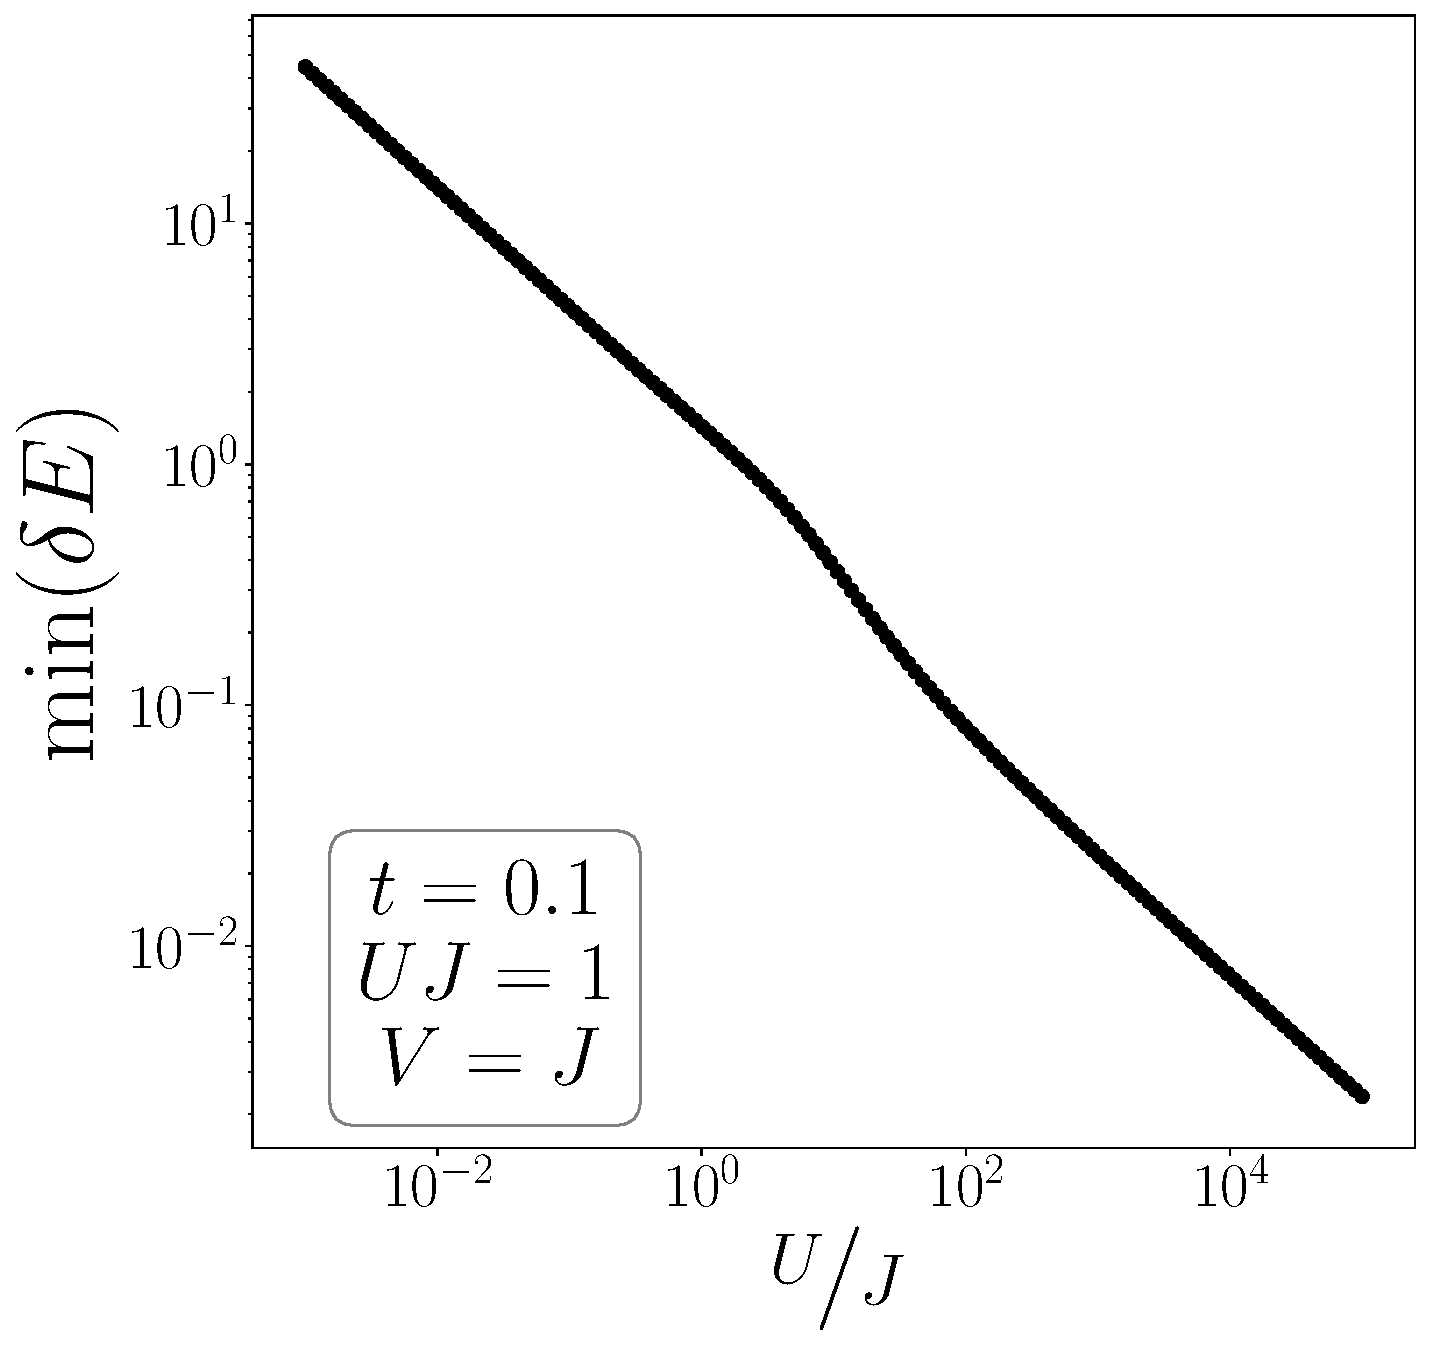
\includegraphics[width=0.32\textwidth]{../figures/gap-t=0.100,J=1_over_U,V=J,N=4,U=0.032,316.228,150.pdf}
	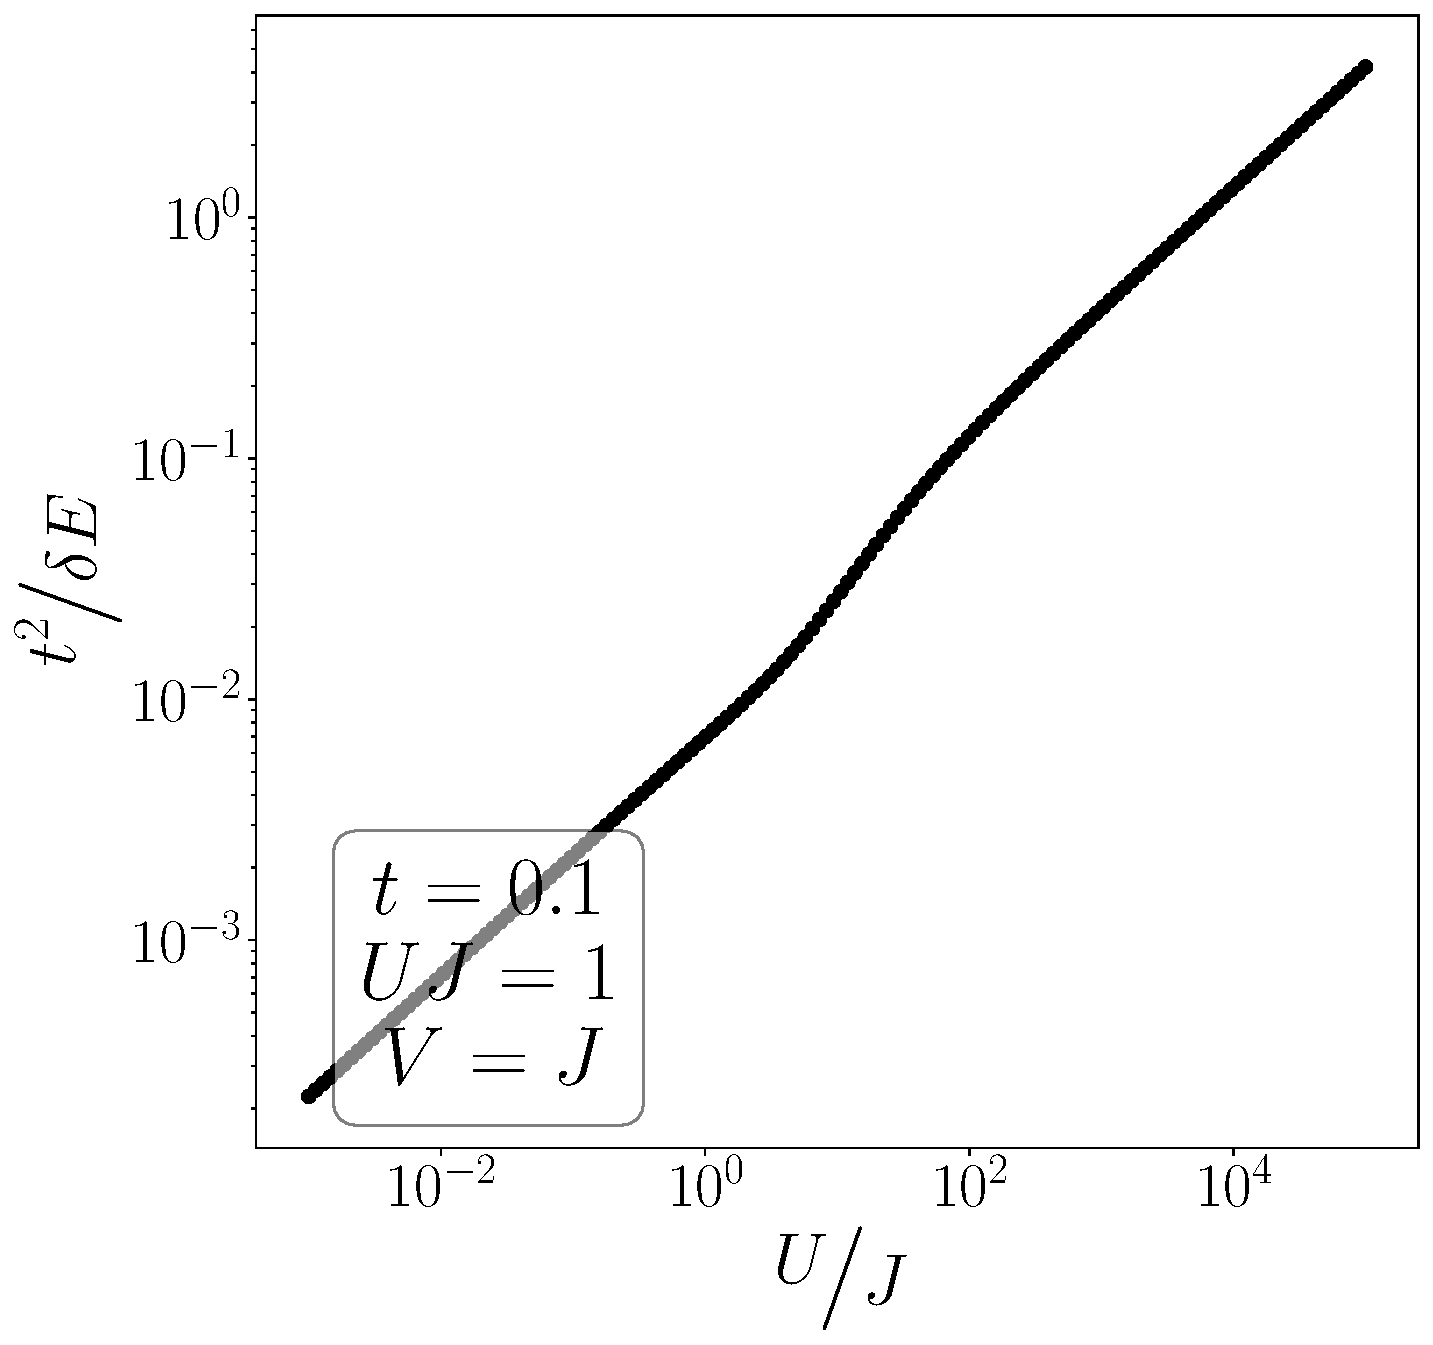
\includegraphics[width=0.32\textwidth]{../figures/par-t=0.100,J=1_over_U,V=J,N=4,U=0.032,316.228,150.pdf}
	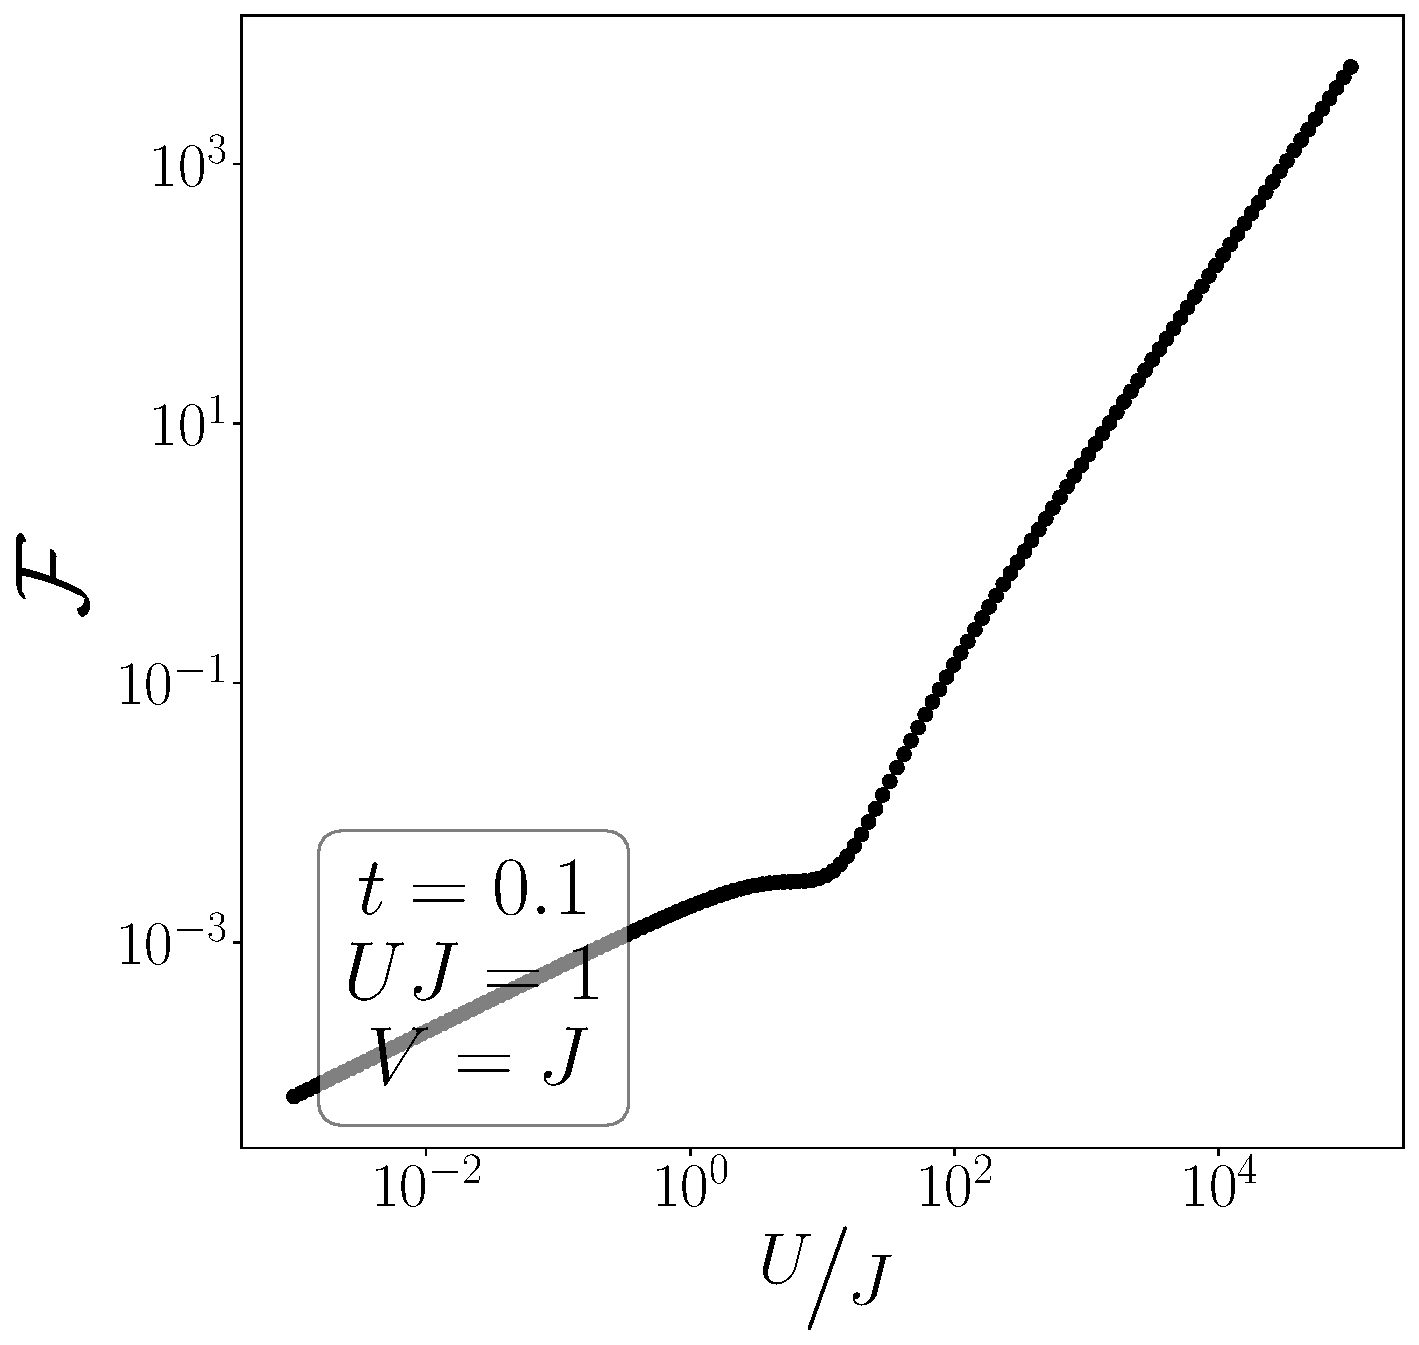
\includegraphics[width=0.32\textwidth]{../figures/lfl-t=0.100,J=1_over_U,V=J,N=4,U=0.032,316.228,150.pdf}
\end{center}
The vanishing of the gap and the growth of the small parameter indicates the breakdown of perturbation theory around the singlet; this simply shows that there is a degeneracy in the local moment regime, and the effective Hamiltonian will have to be obtained using degenerate perturbation theory. The presence of degeneracy also suggests that the effective Hamiltonian will be of the non-Fermi liquid type.

\subsubsection*{\large Behaviour of mutual information within the Kondo cloud}
\begin{center}
	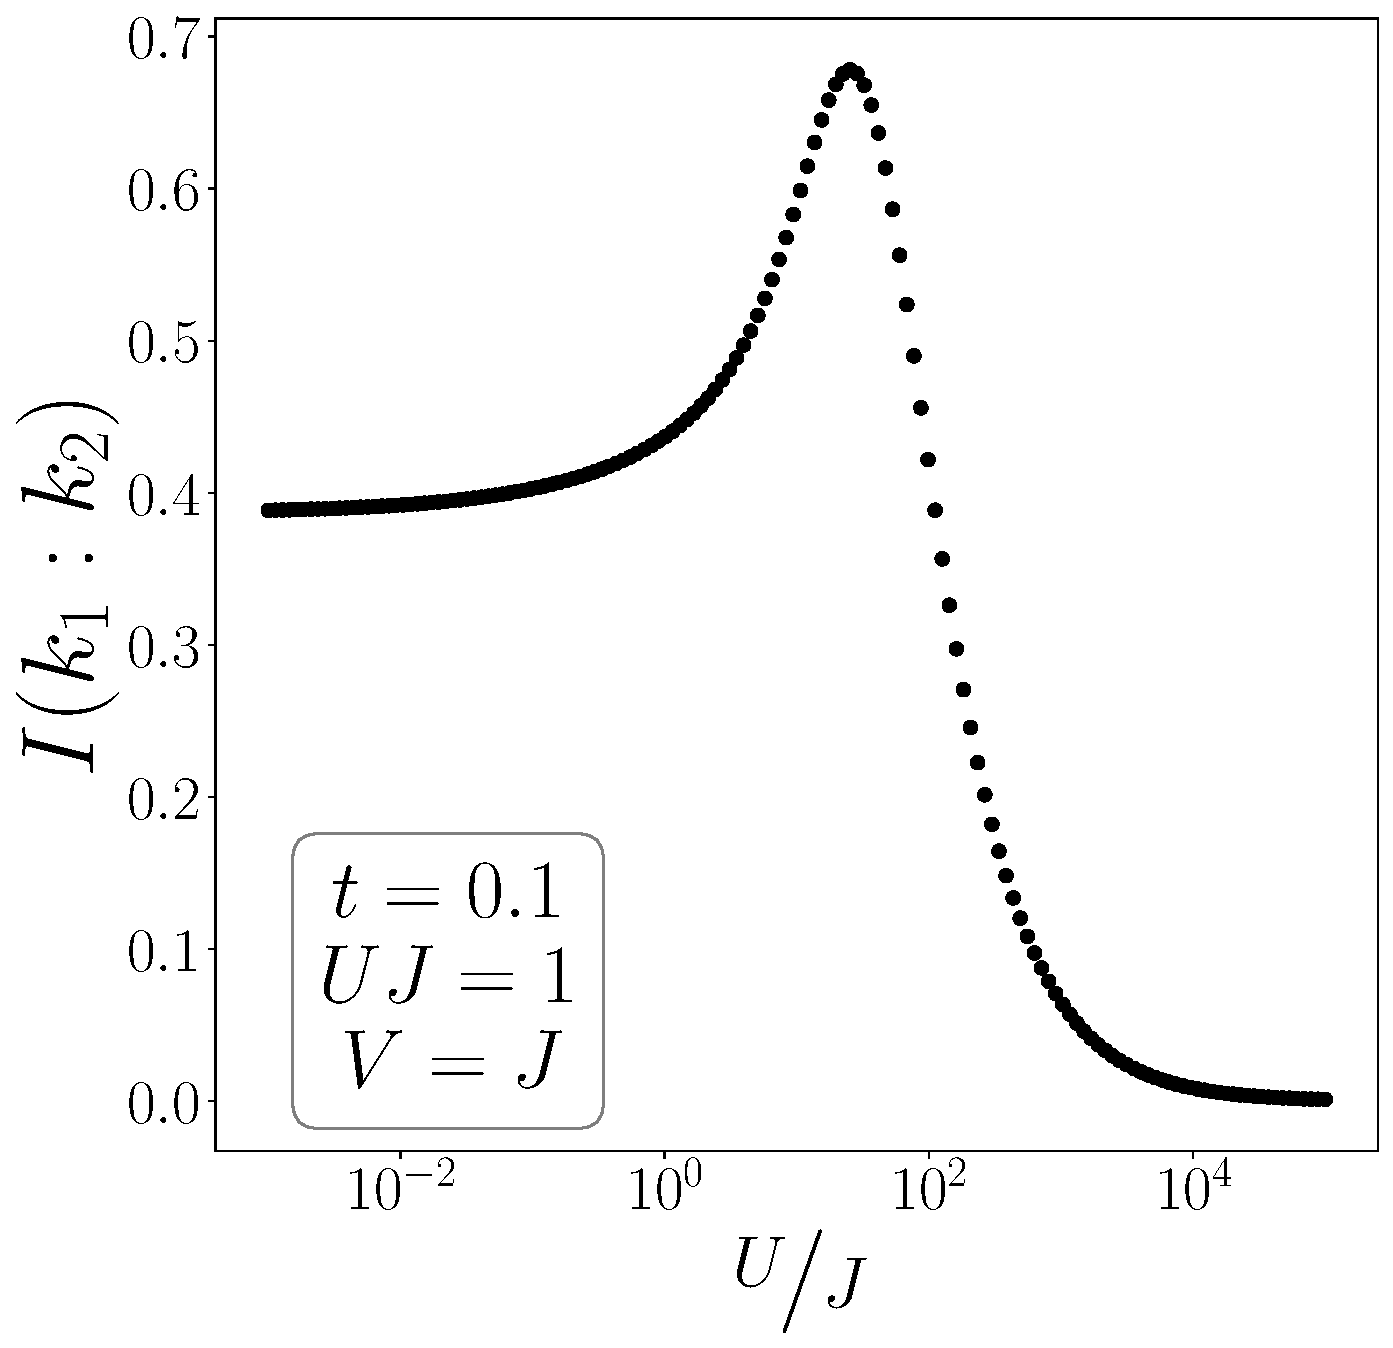
\includegraphics[width=0.32\textwidth]{../figures/corr-k-t=0.100,J=1_over_U,V=J,N=4,U=0.032,316.228,150.pdf}
\end{center}
The vanishing of the Kondo cloud at large \(U/J\) is clear indication of the destruction of the Kondo cloud and the breakdown of screening. Non-zero mutual information indicates an (impurity-mediated) interaction between the \(k-\)states of the conduction bath; seen differently, it is this interaction that is responsively for the screening of the impurity. The disappearance of the mutual information is indicative of the disappearance of this interaction.

\subsubsection*{\large Behaviour of mutual information between various real space members}
\begin{center}
	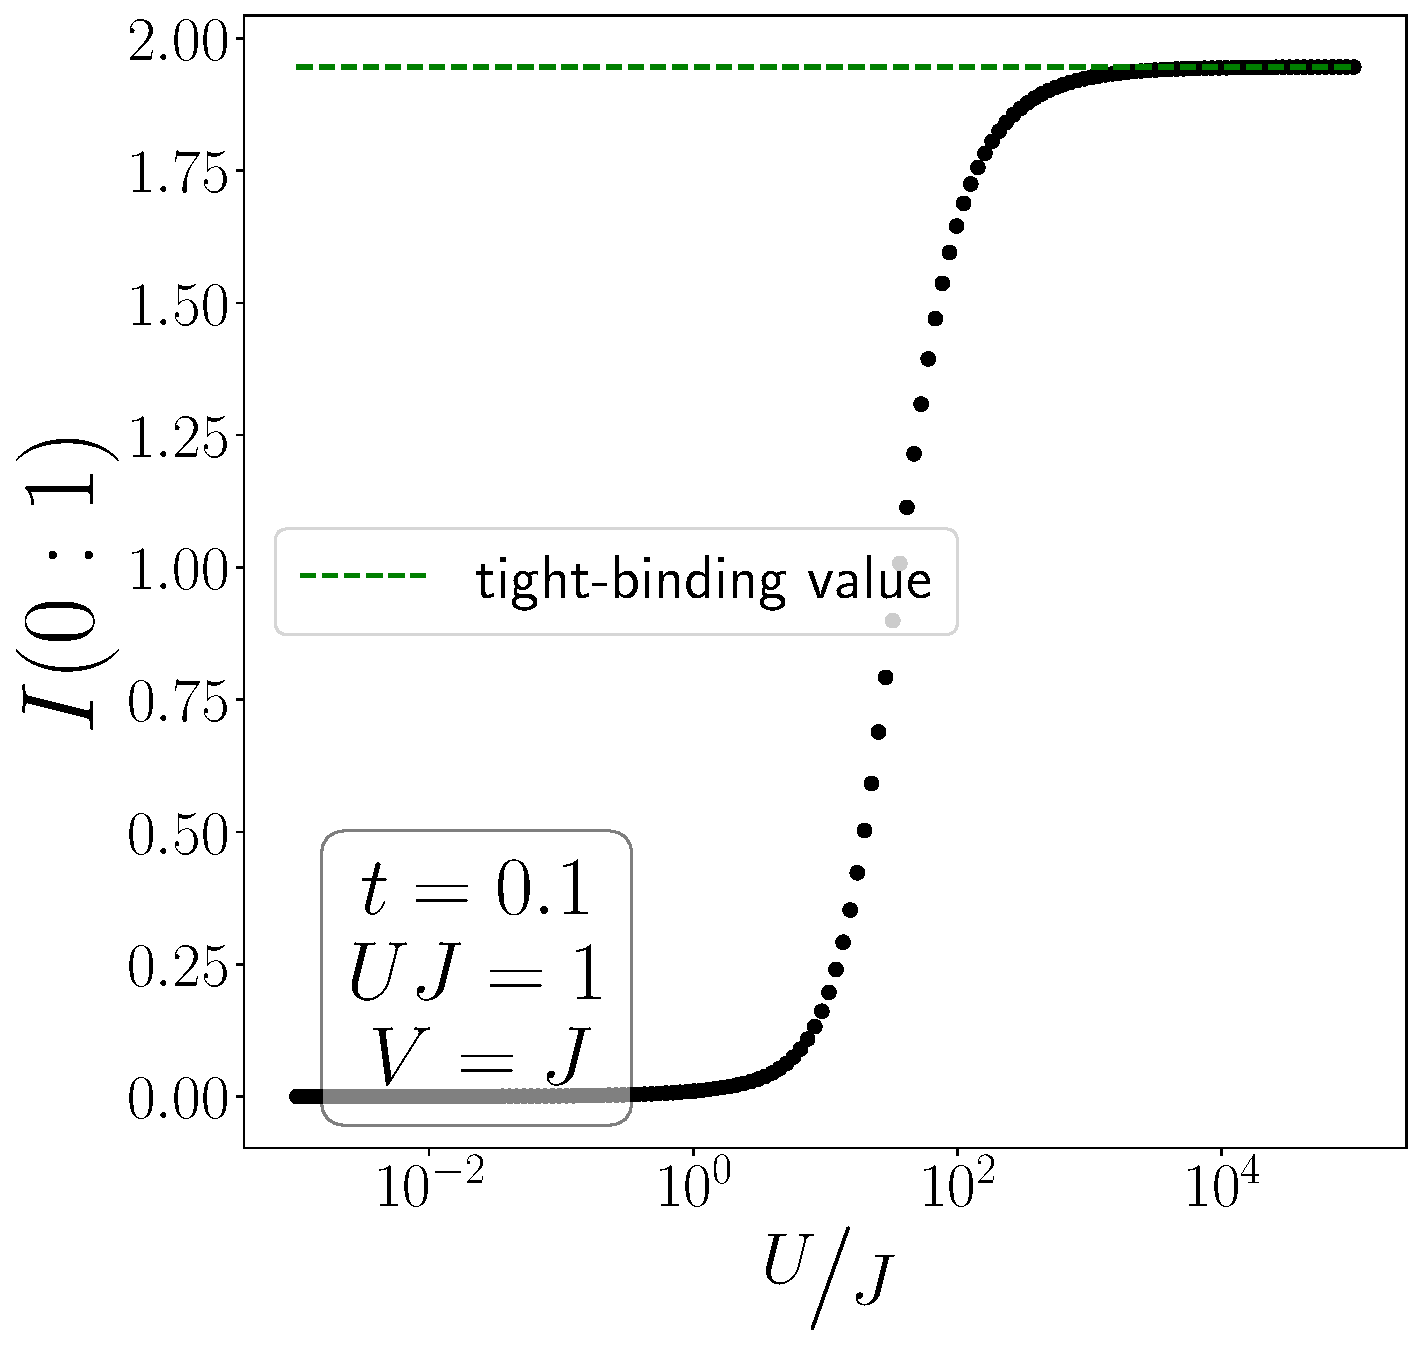
\includegraphics[width=0.32\textwidth]{../figures/mi-01-t=0.100,J=1_over_U,V=J,N=4,U=0.032,316.228,150.pdf}
	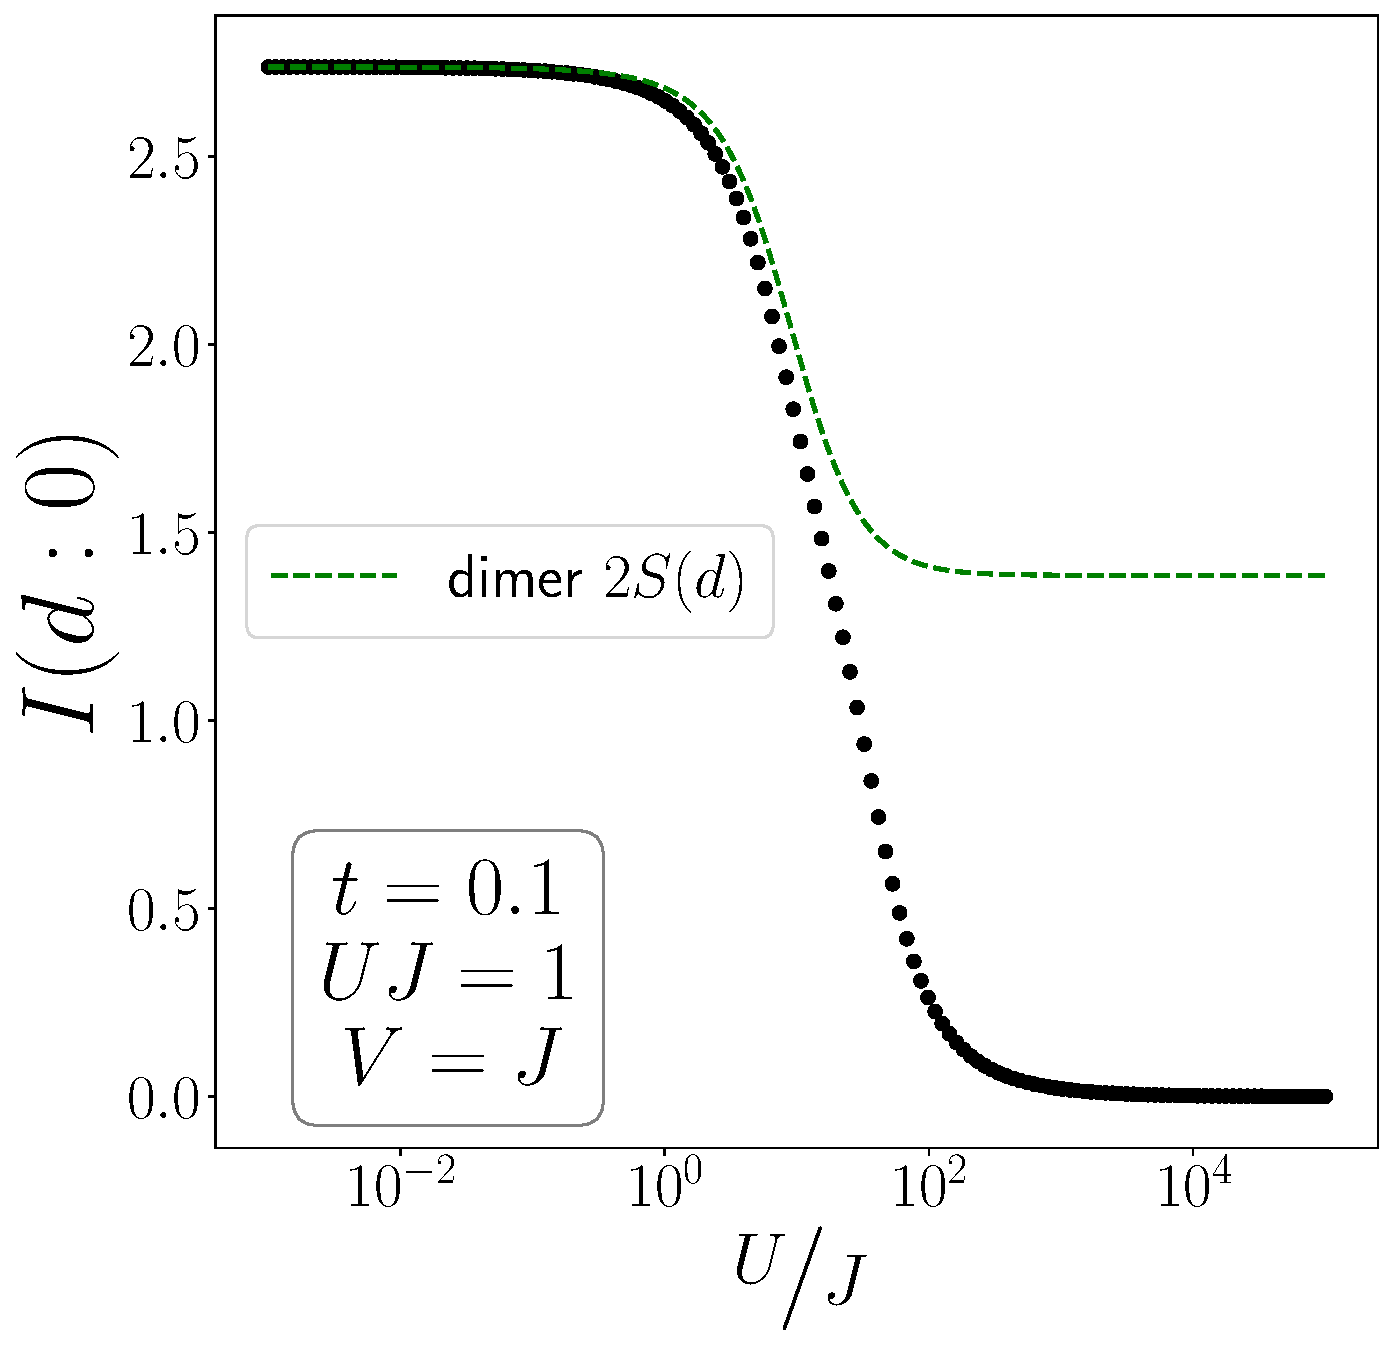
\includegraphics[width=0.32\textwidth]{../figures/mi-d0-t=0.100,J=1_over_U,V=J,N=4,U=0.032,316.228,150.pdf}
	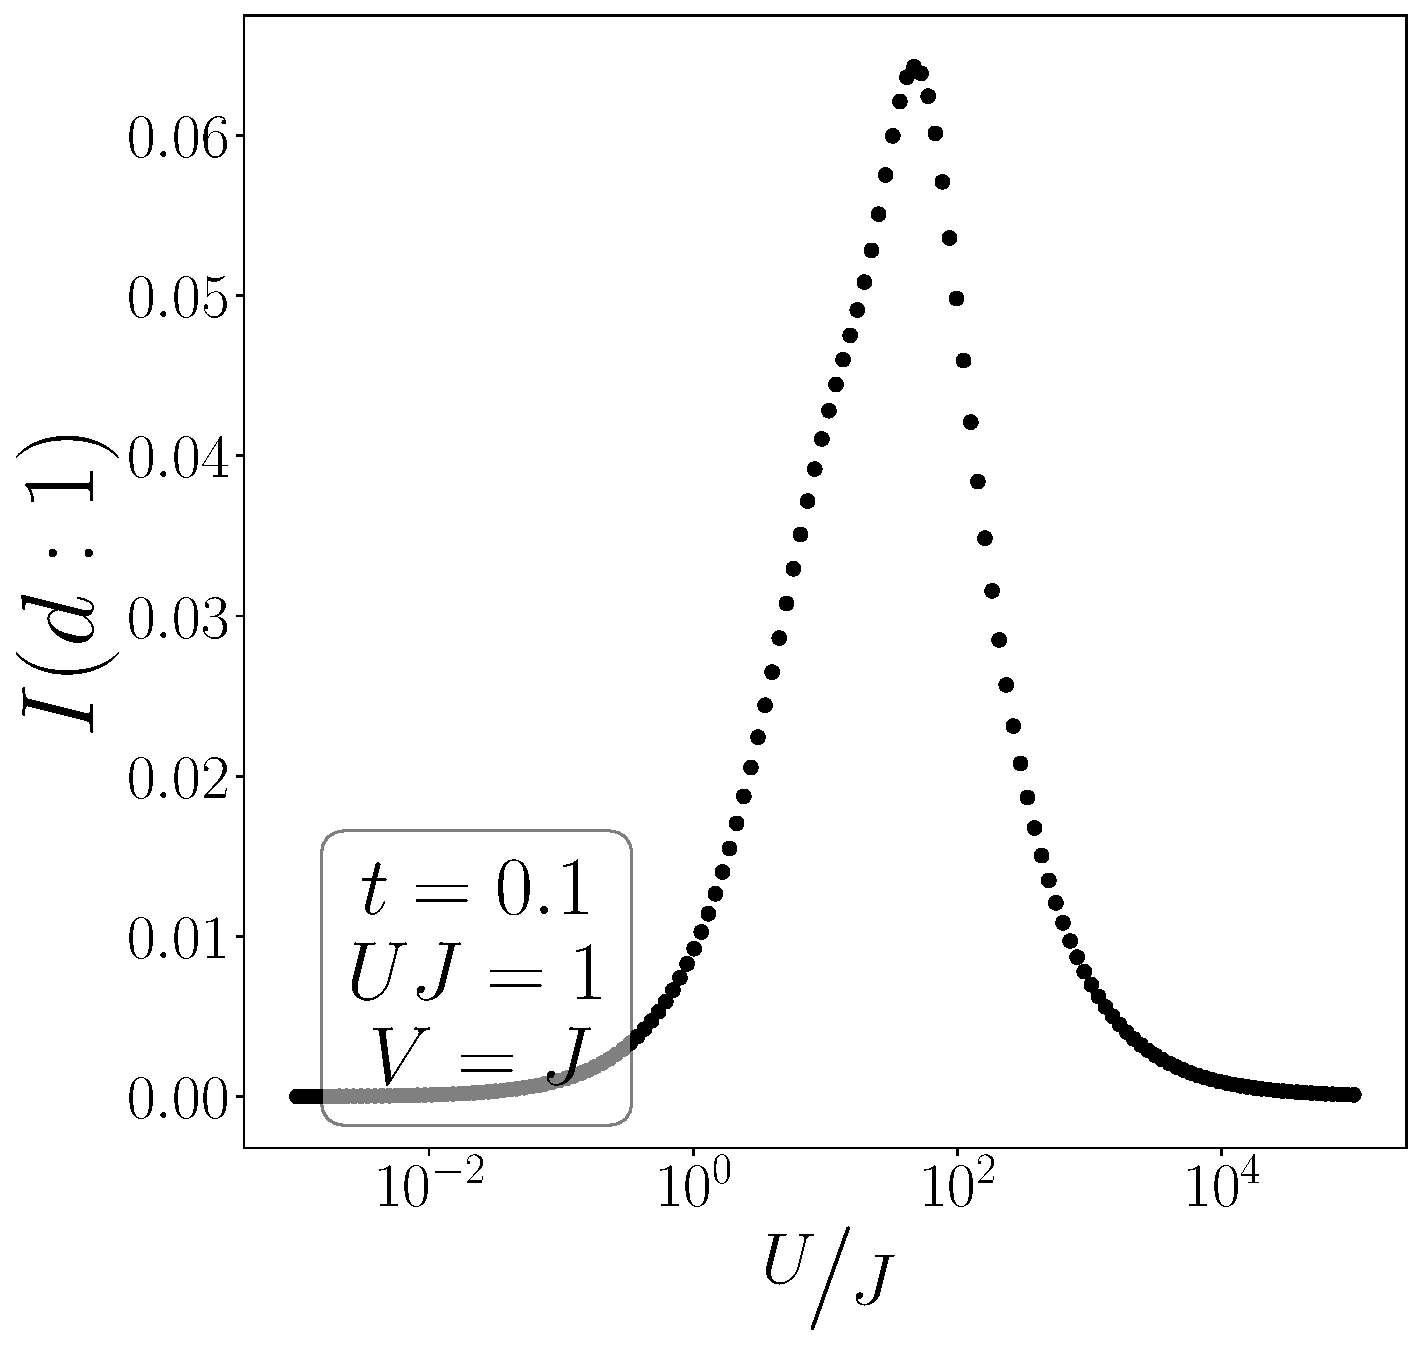
\includegraphics[width=0.32\textwidth]{../figures/mi-d1-t=0.100,J=1_over_U,V=J,N=4,U=0.032,316.228,150.pdf}
\end{center}
The impurity-zeroth site mutual information \(I(d:0)\) remains unchanged at the maximum for an appreciable range of values, and this shows the stability of the singlet. Meanwhile, the mutual information between the zeroth site and the site nearest to it (\(I(0:1)\)) grows, because when the singlet weakens, the zeroth site is able to entangle more with the other sites. It finally saturates to its maximum value, which is the value produced as result of the tight-binding hopping. The mutual information between the impurity and sites beyond the zeroth site (\(I(d:1)\)) show a non-monotonic behaviour; it first increases as the entanglement that was initially restricted to just the impurity and the zeroth sites begins "seeping" into the other sites as well. Beyond a critical value of \(U/J\), \(I(d:1)\) starts dropping, because the entanglement has now mostly shifted out of the zero mode and into the conduction bath.

\subsubsection*{\large Behaviour of impurity entanglement entropy}

\begin{center}
	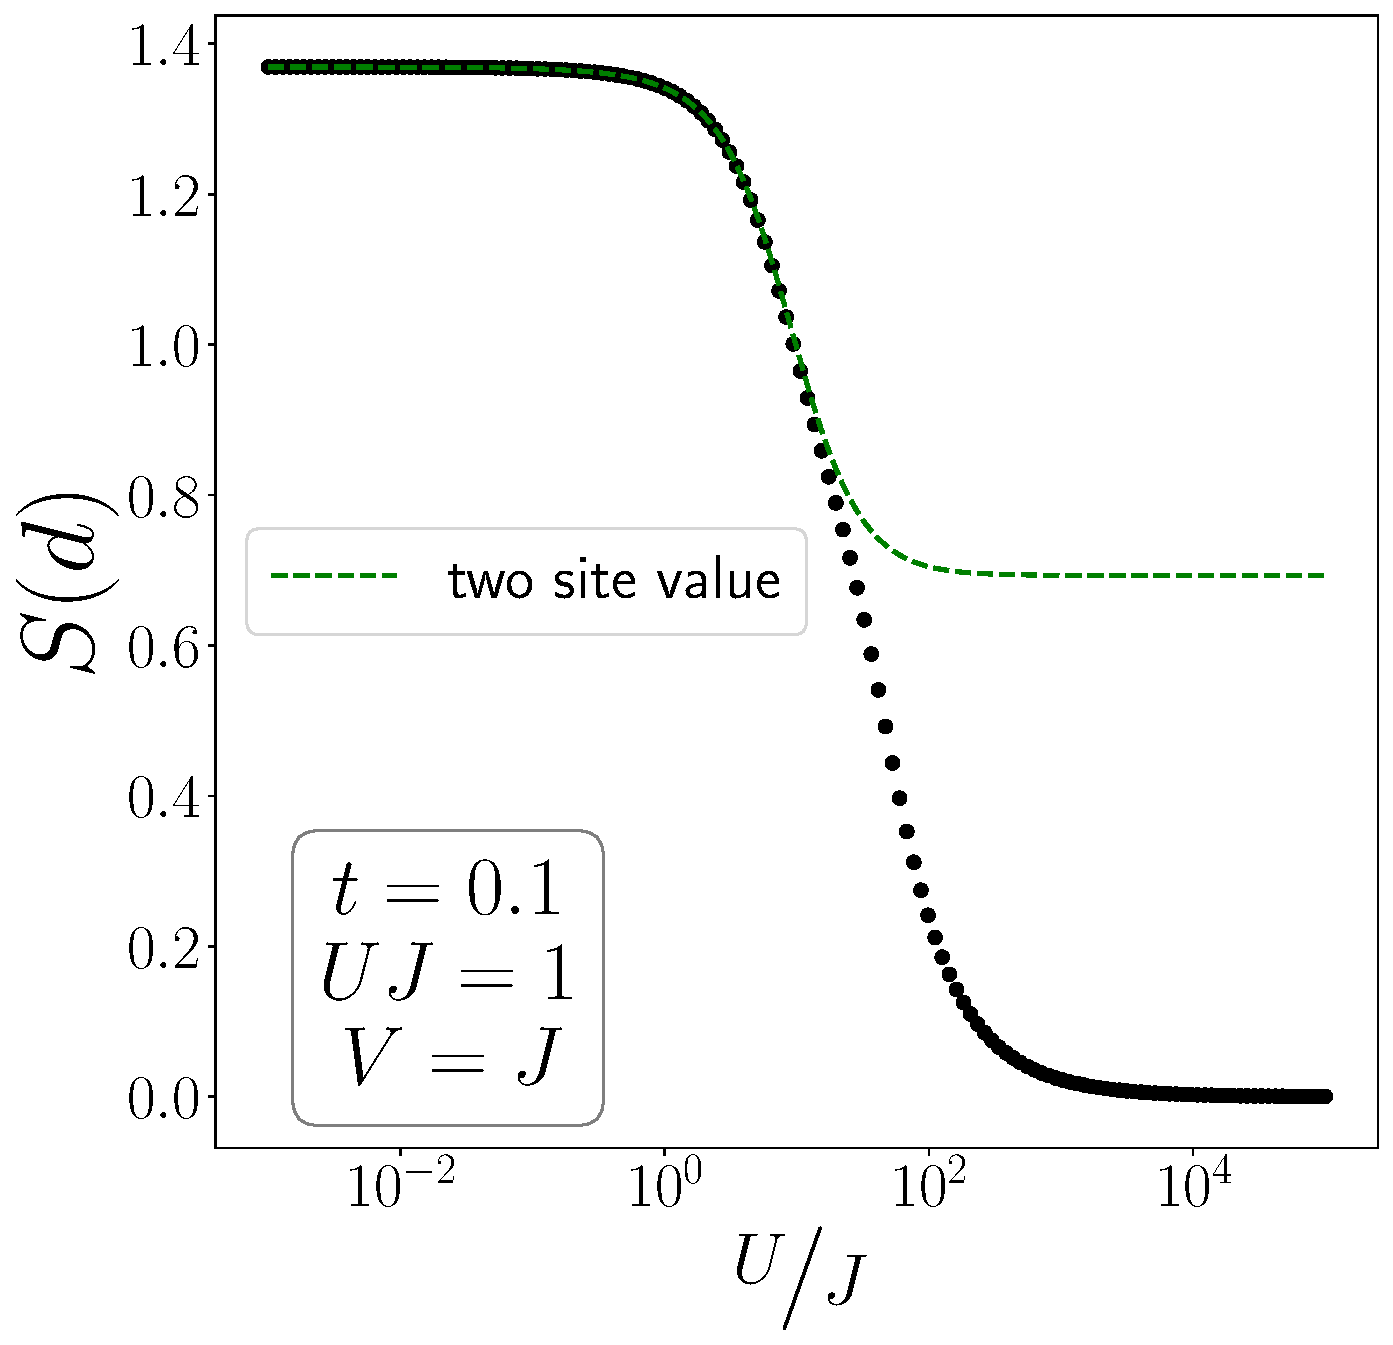
\includegraphics[width=0.35\textwidth]{../figures/EE-d-t=0.100,J=1_over_U,V=J,N=4,U=0.032,316.228,150.pdf}
\end{center}

The von-Neumann entanglement entropy \(S(d)\) of the impurity shows pretty straightforward behaviour. It is maximum for \(U \ll J\) because it is in a singlet configuration. For \(U \gg J\), the singlet weakens and the impurity begins to decouple from the bath, leading to a reduction in \(S(d)\). At sufficiently low values of \(J/U\), the impurity decouples from the zeroth site and the total system can be factorised into a local moment in product with a tight-binding chain, so that the impurity site will now have zero entanglement entropy.

\subsubsection*{\large Behaviour of spin-spin correlations}
\begin{center}
	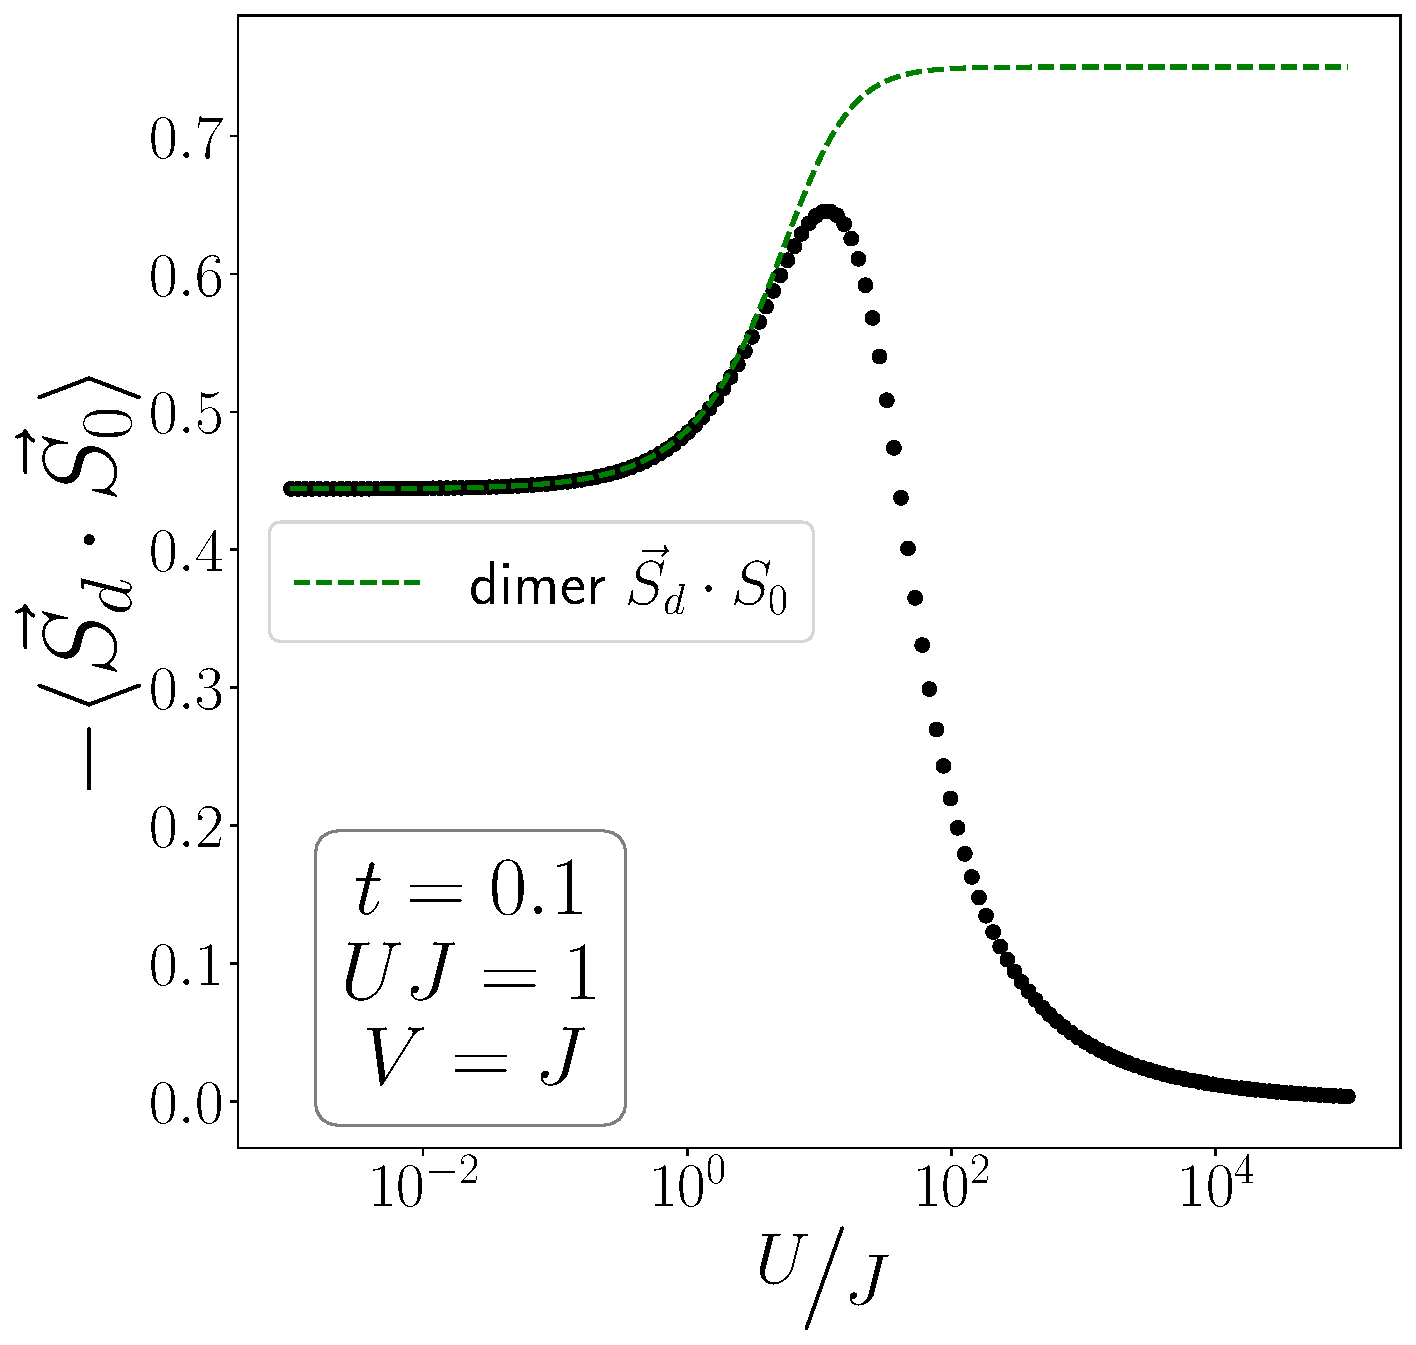
\includegraphics[width=0.32\textwidth]{../figures/corr-d0-t=0.100,J=1_over_U,V=J,N=4,U=0.032,316.228,150.pdf}
	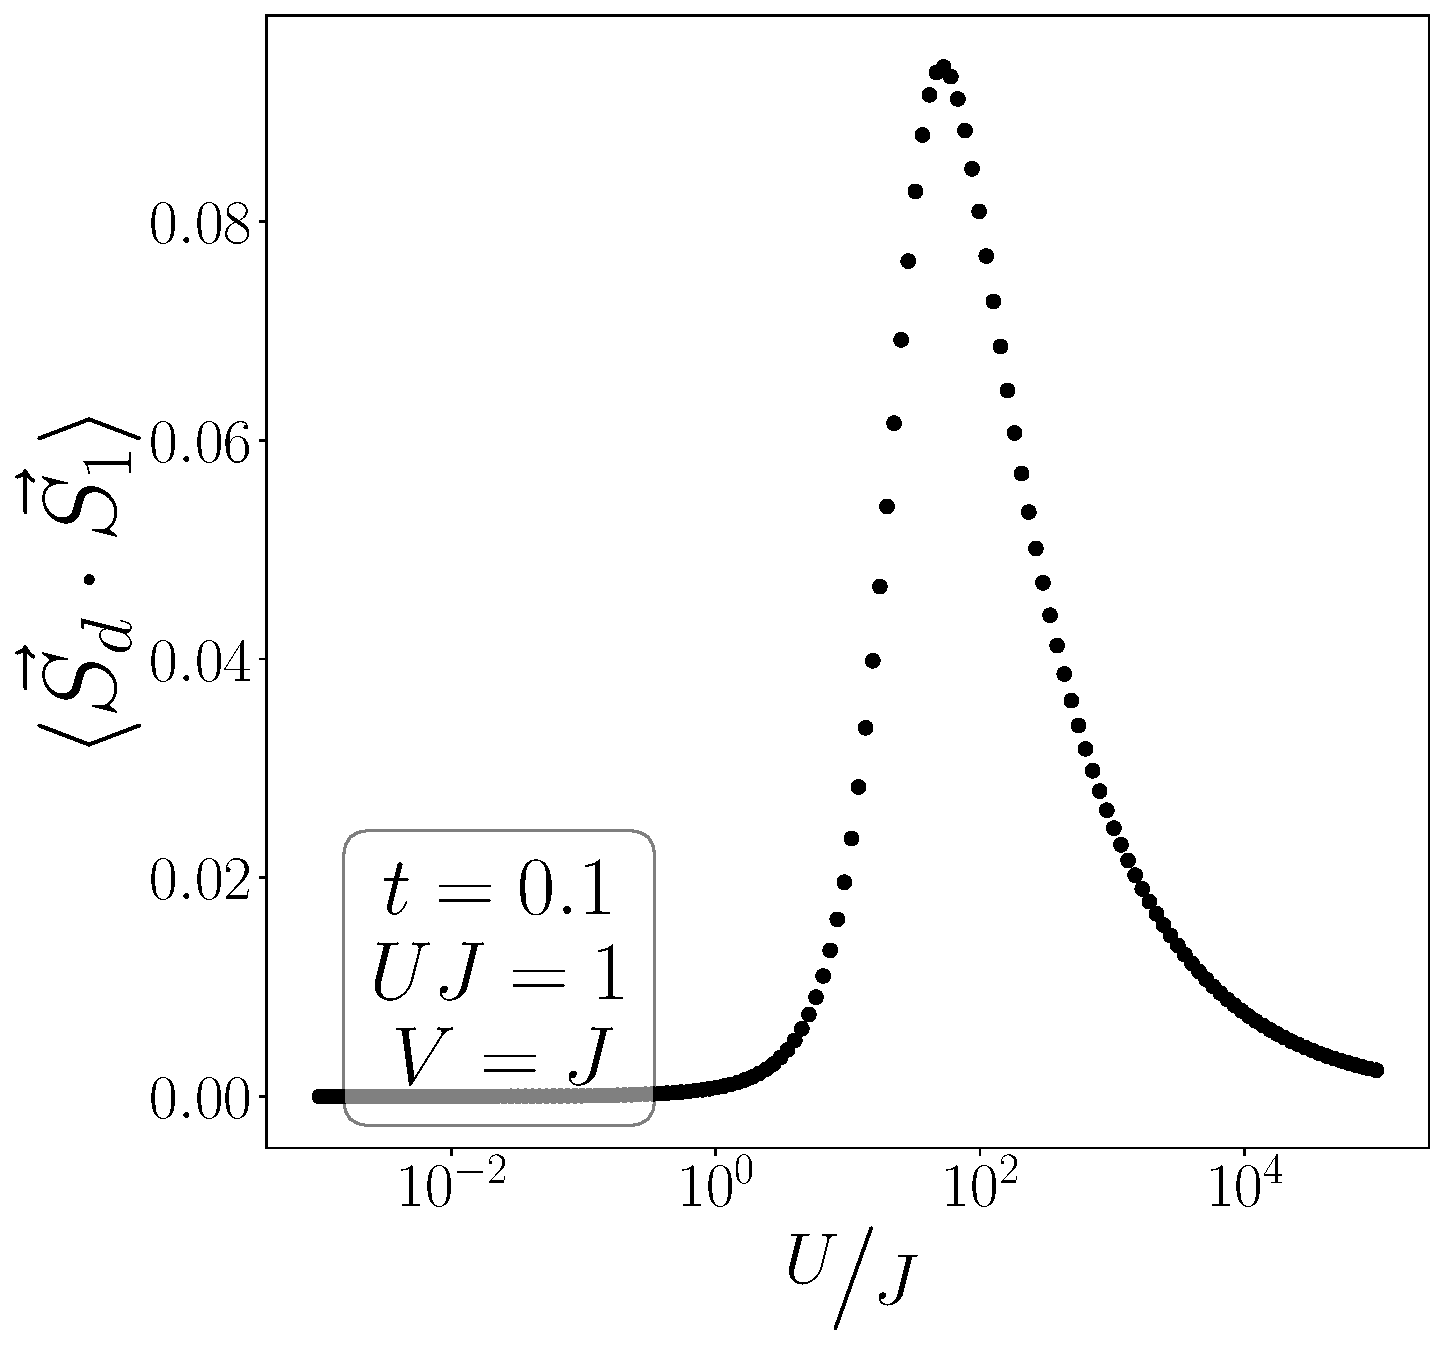
\includegraphics[width=0.32\textwidth]{../figures/corr-d1-t=0.100,J=1_over_U,V=J,N=4,U=0.032,316.228,150.pdf}
\end{center}

\subsubsection*{\Large Plots for 6 sites}
\begin{center}
	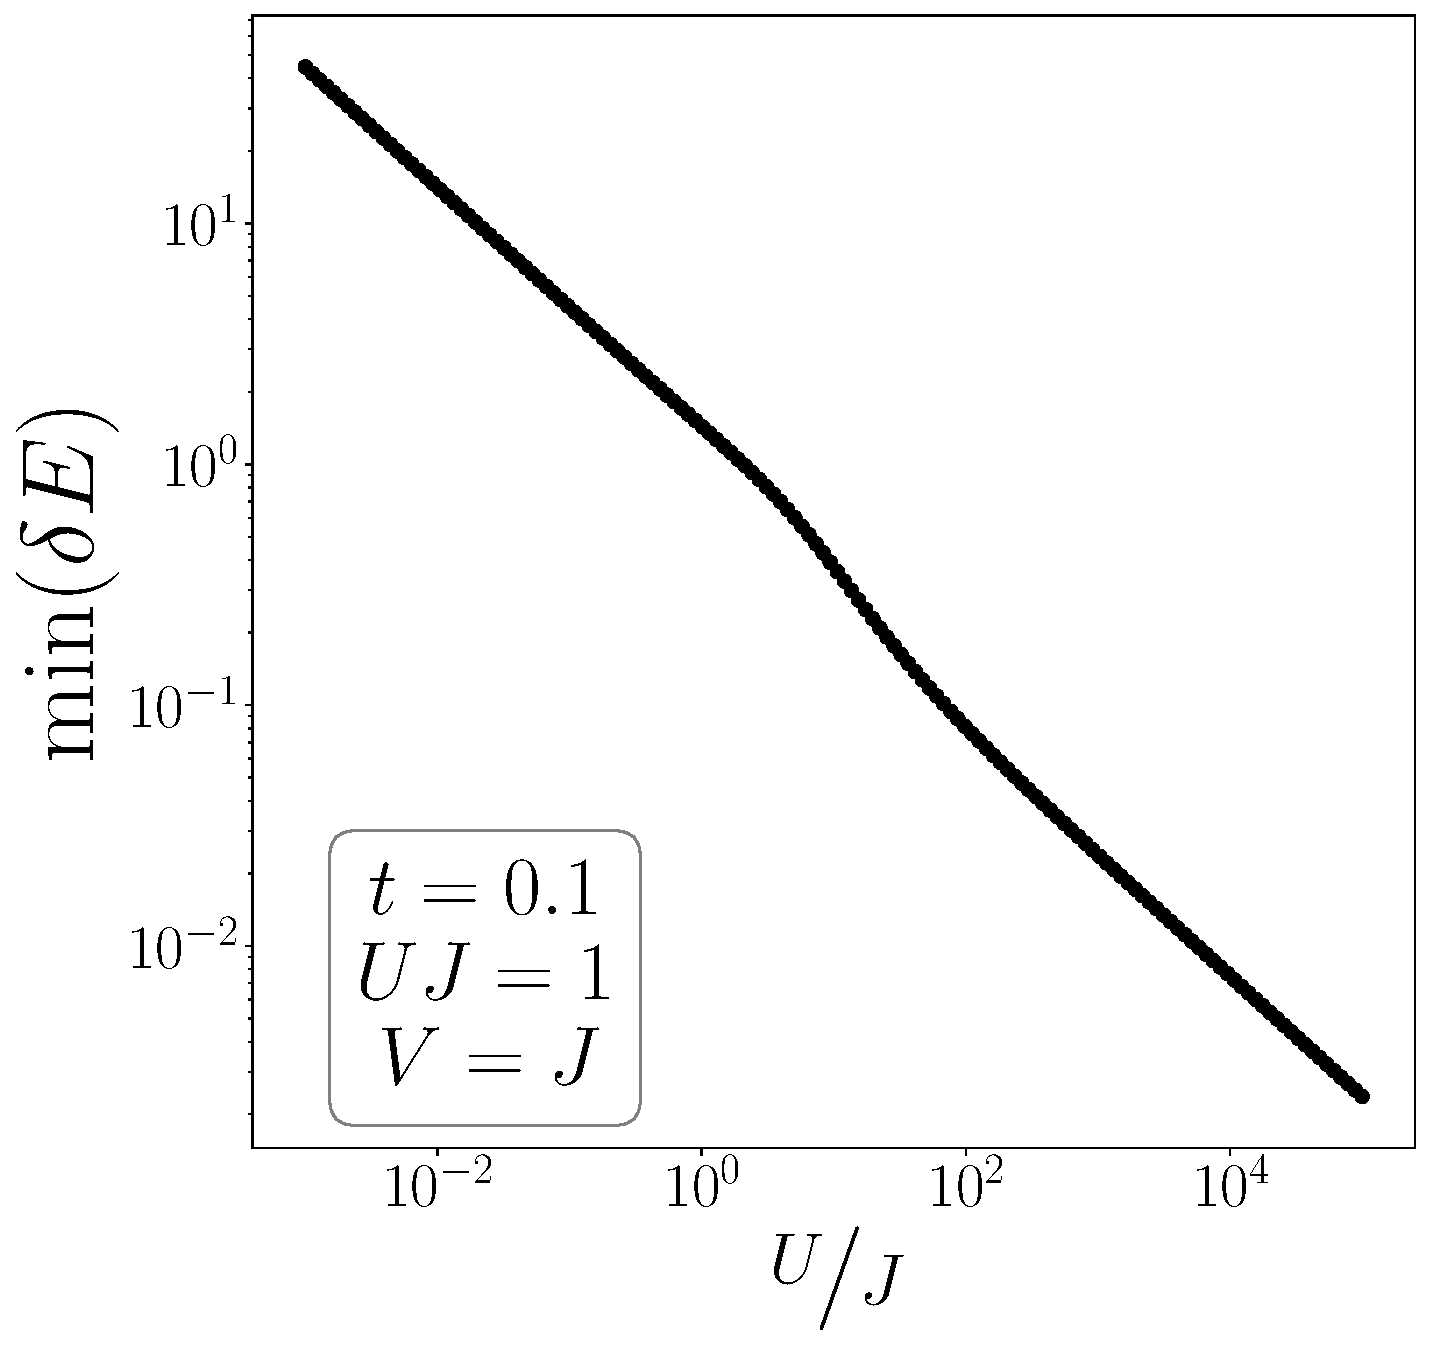
\includegraphics[width=0.32\textwidth]{../figures/gap-t=0.100,J=1_over_U,V=J,N=6,U=0.032,316.228,150.pdf}
	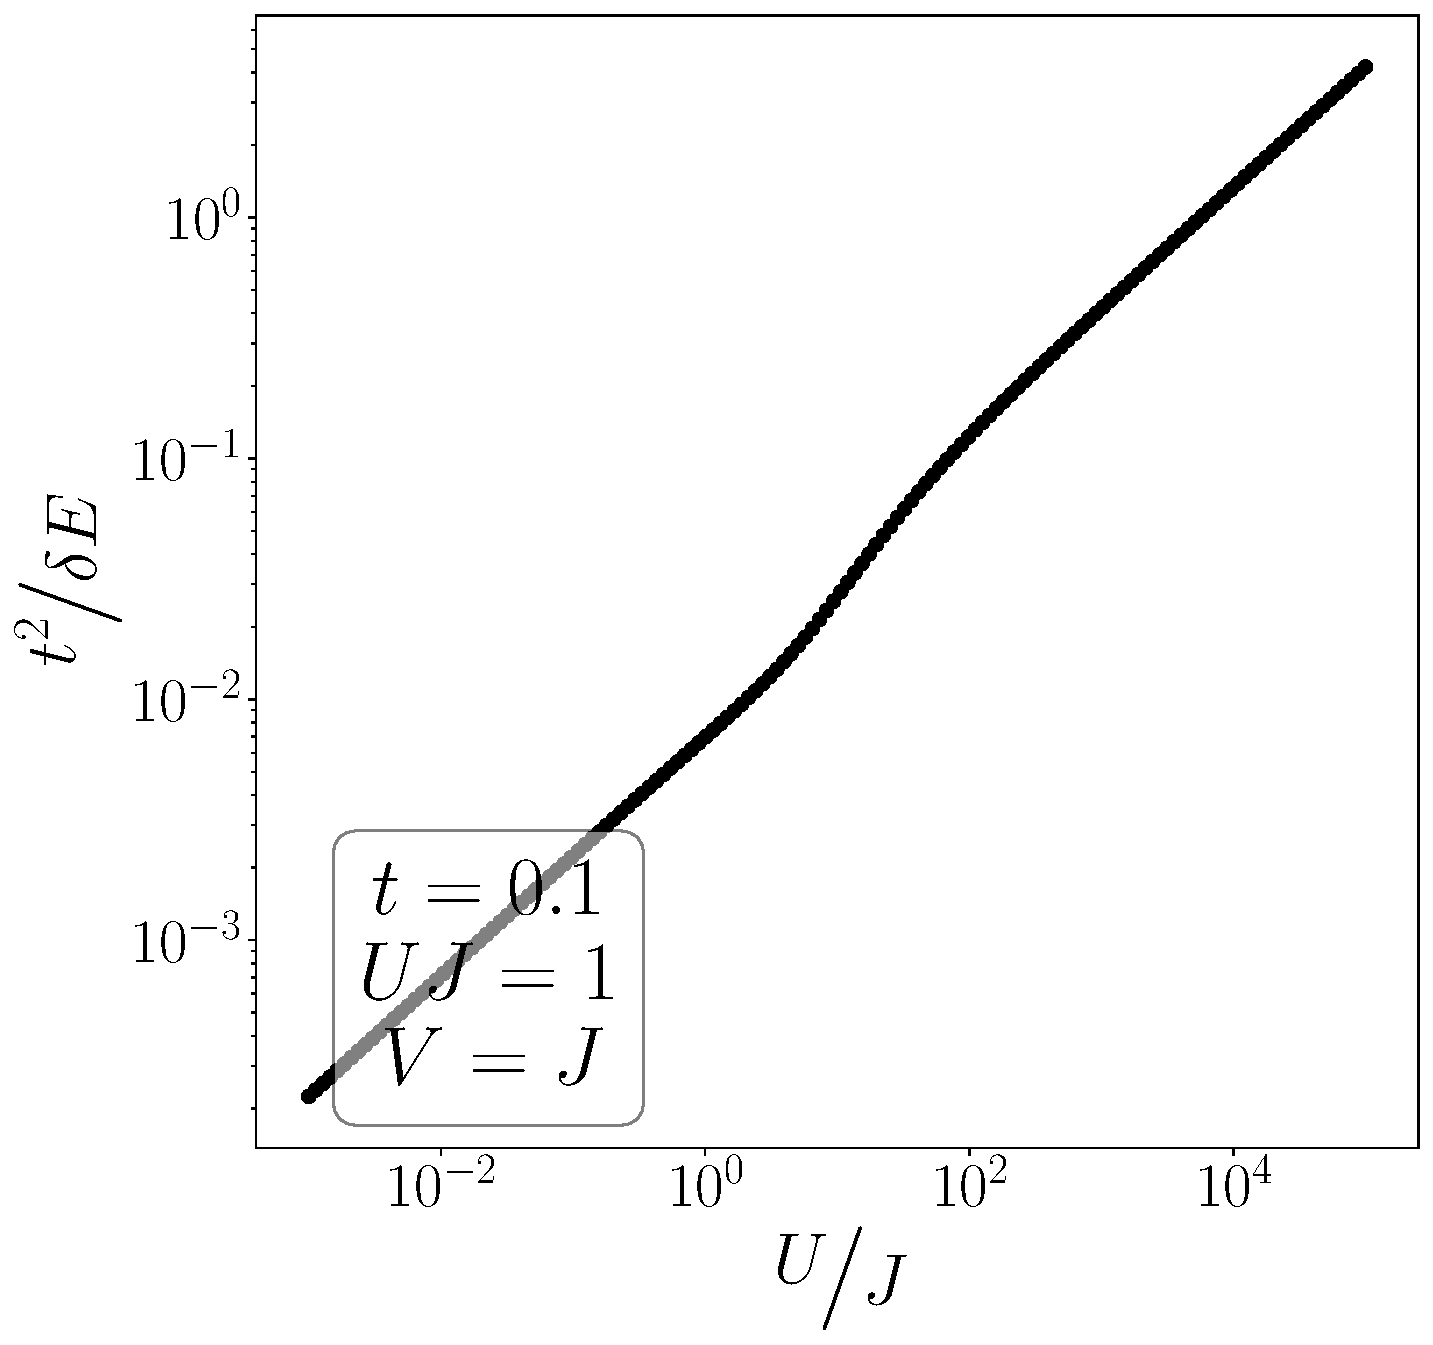
\includegraphics[width=0.32\textwidth]{../figures/par-t=0.100,J=1_over_U,V=J,N=6,U=0.032,316.228,150.pdf}
	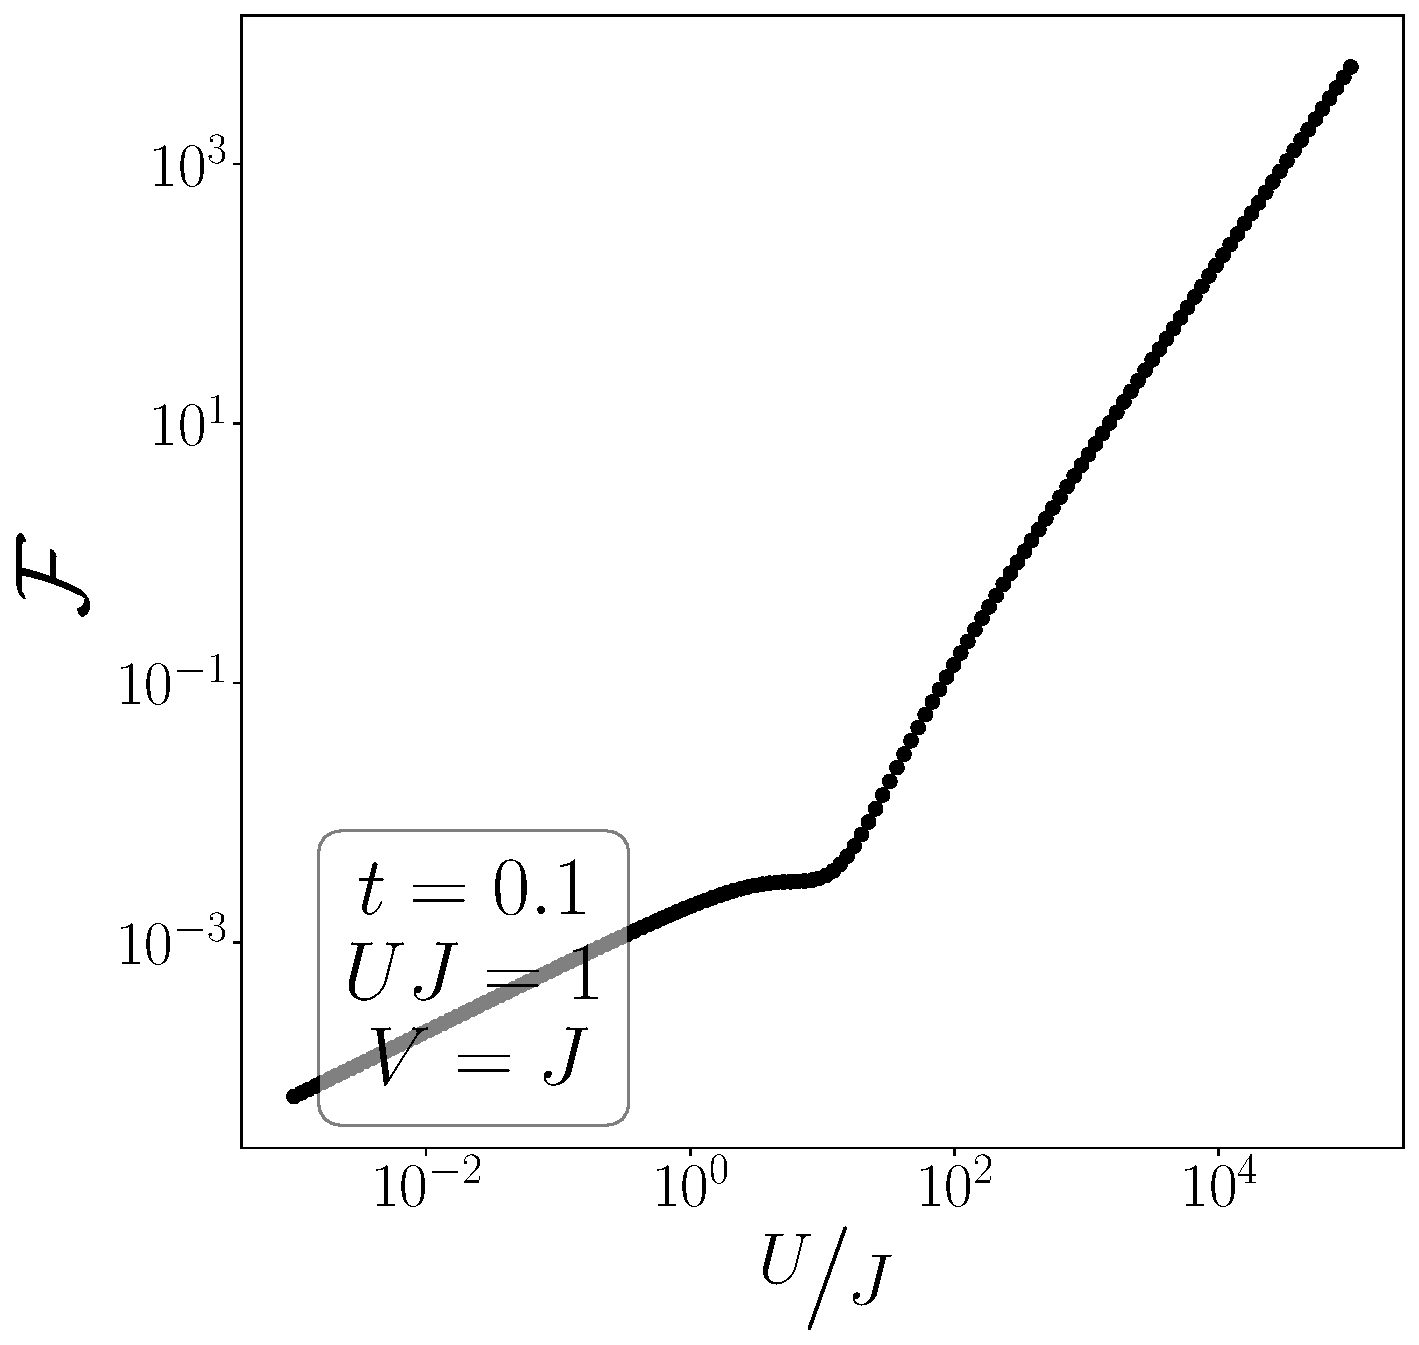
\includegraphics[width=0.32\textwidth]{../figures/lfl-t=0.100,J=1_over_U,V=J,N=6,U=0.032,316.228,150.pdf}
	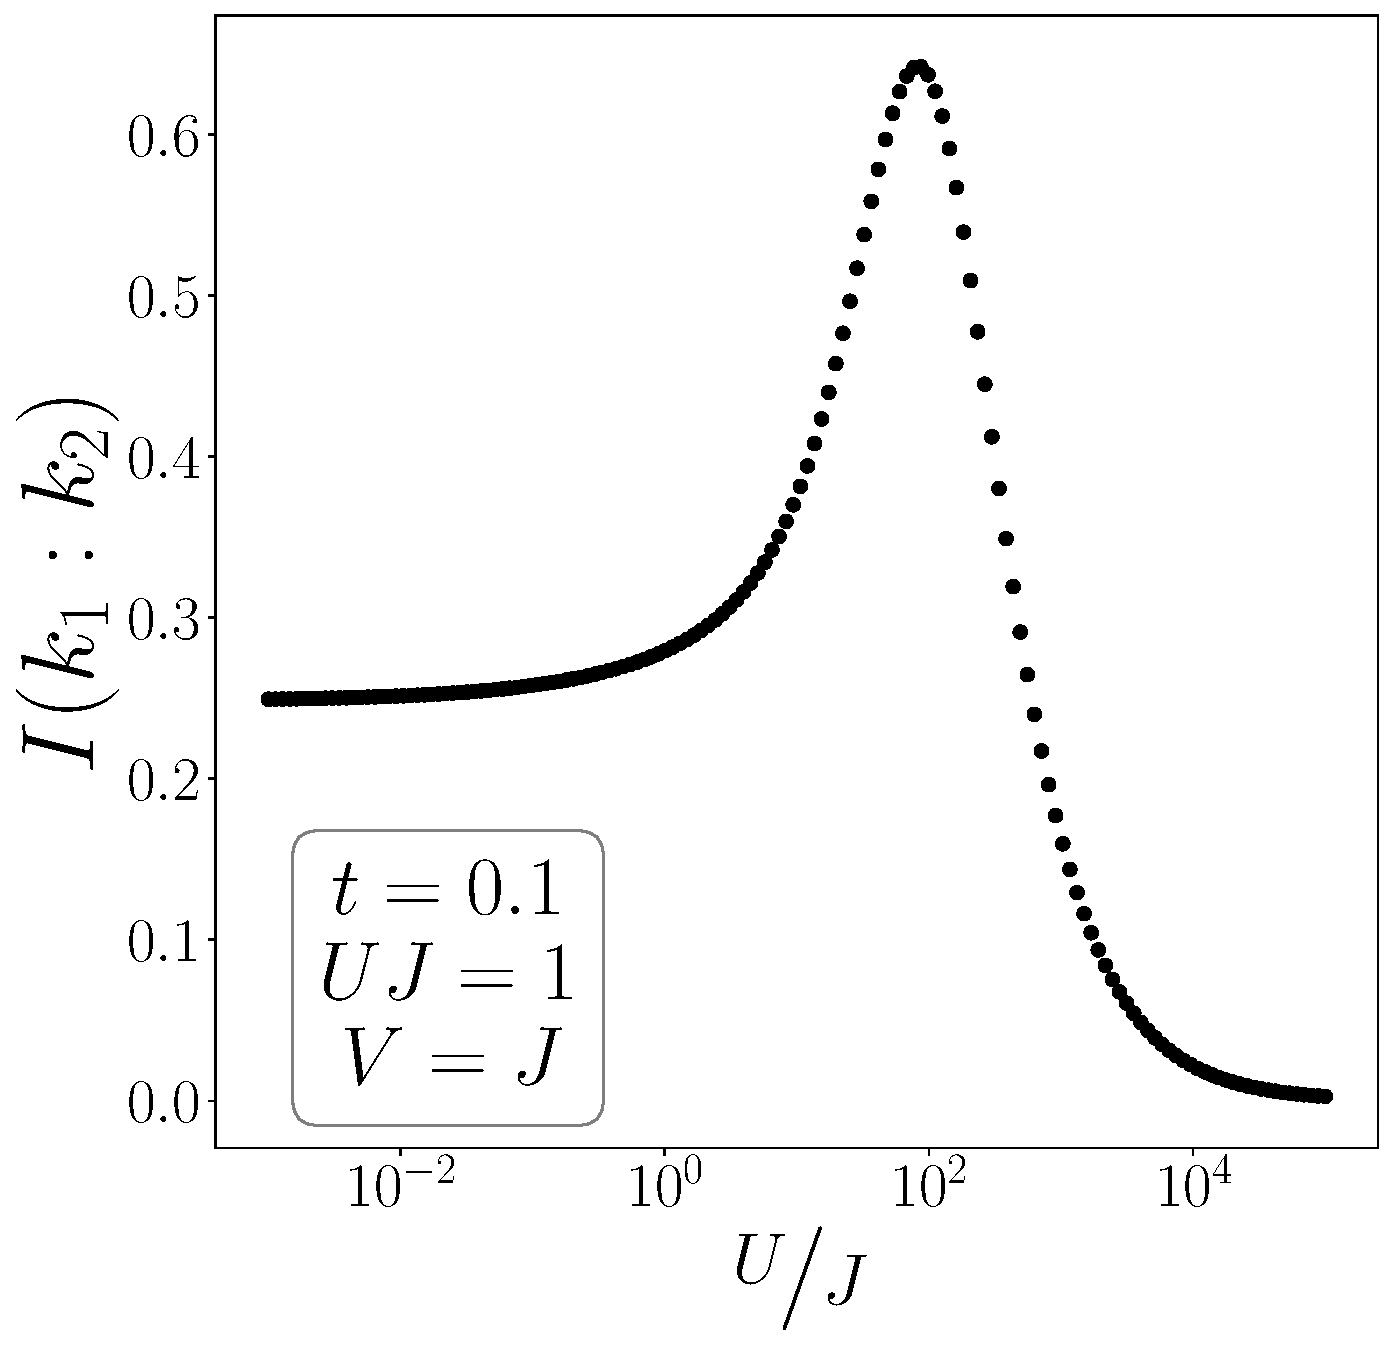
\includegraphics[width=0.32\textwidth]{../figures/corr-k-t=0.100,J=1_over_U,V=J,N=6,U=0.032,316.228,150.pdf}
	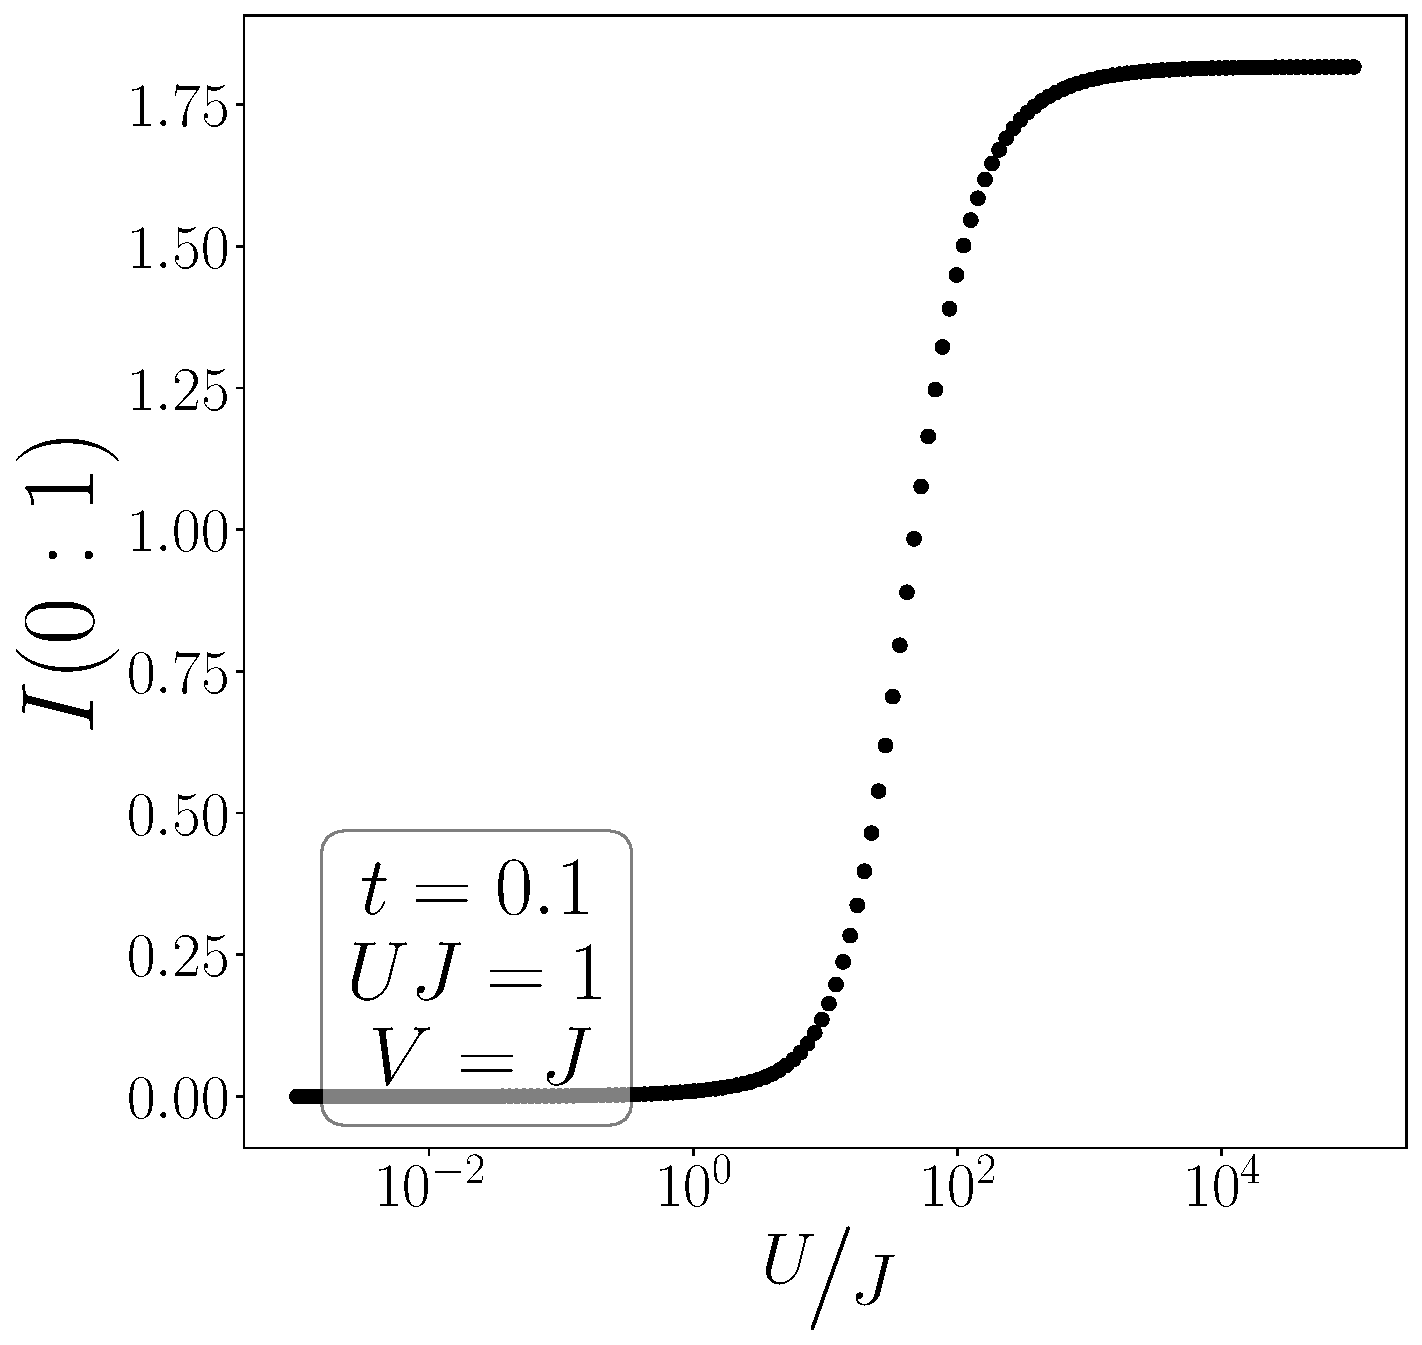
\includegraphics[width=0.32\textwidth]{../figures/mi-01-t=0.100,J=1_over_U,V=J,N=6,U=0.032,316.228,150.pdf}
	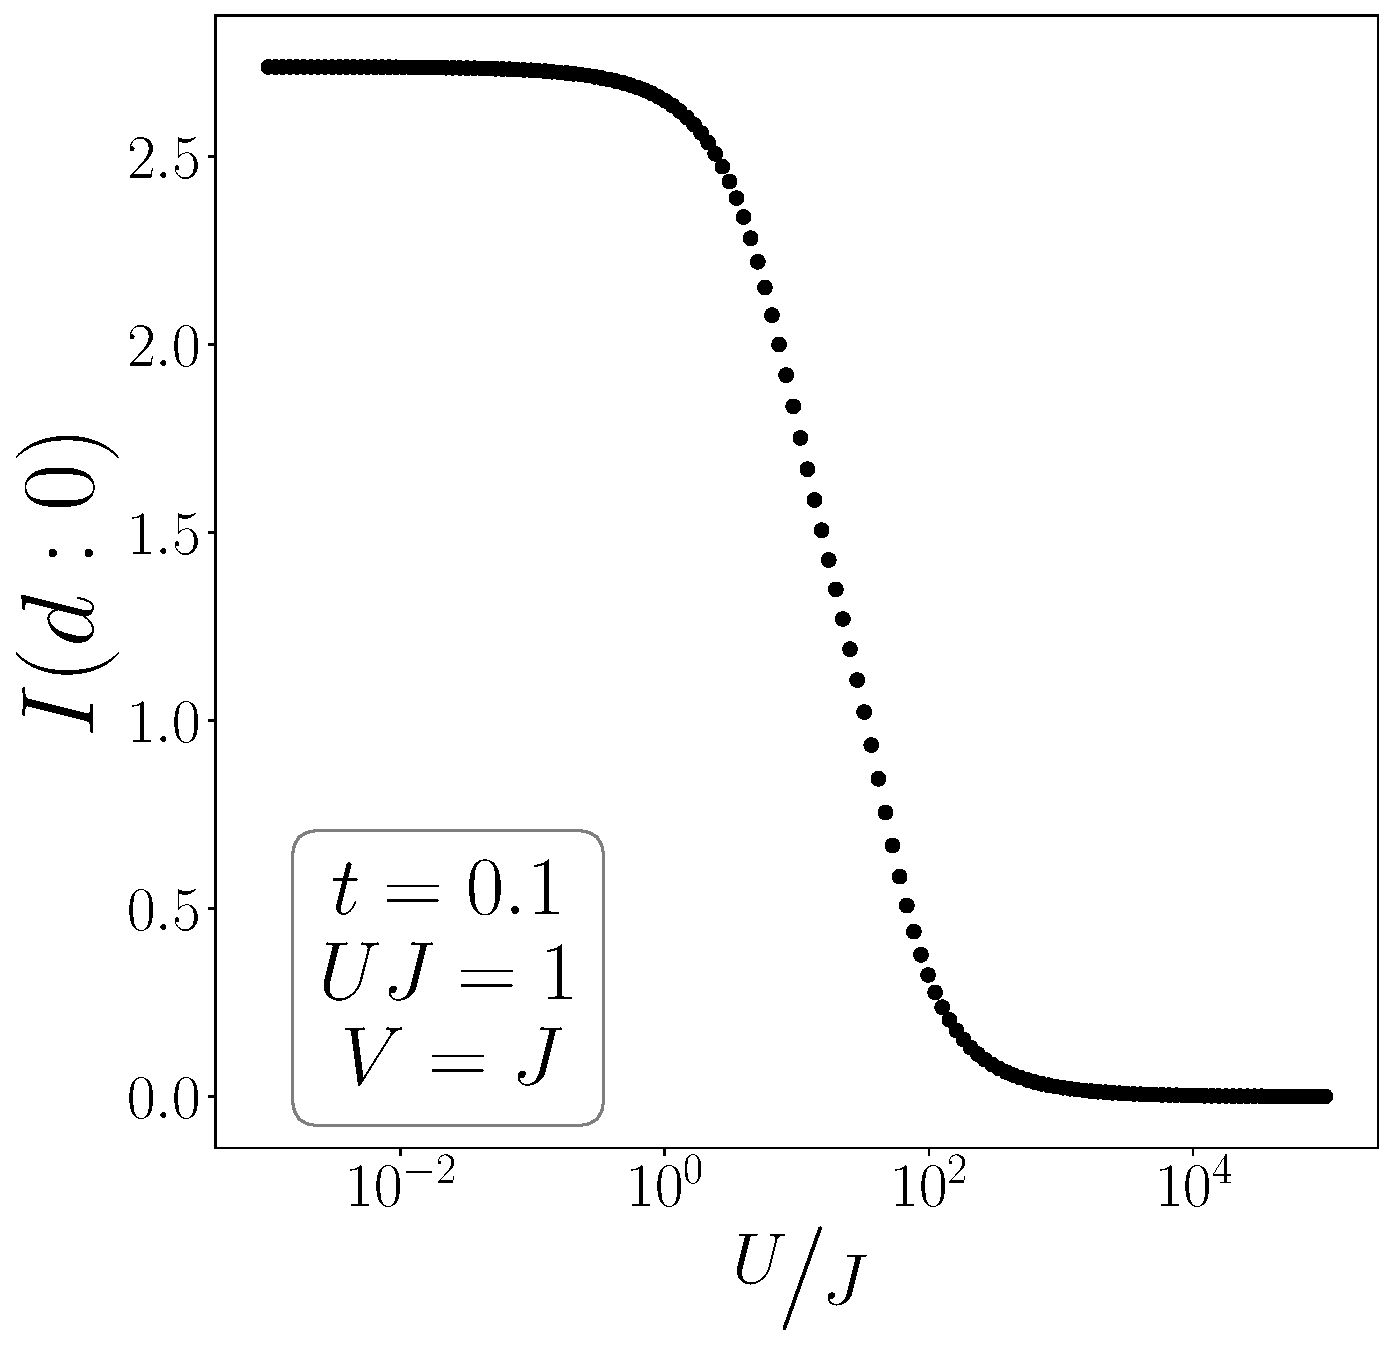
\includegraphics[width=0.32\textwidth]{../figures/mi-d0-t=0.100,J=1_over_U,V=J,N=6,U=0.032,316.228,150.pdf}
	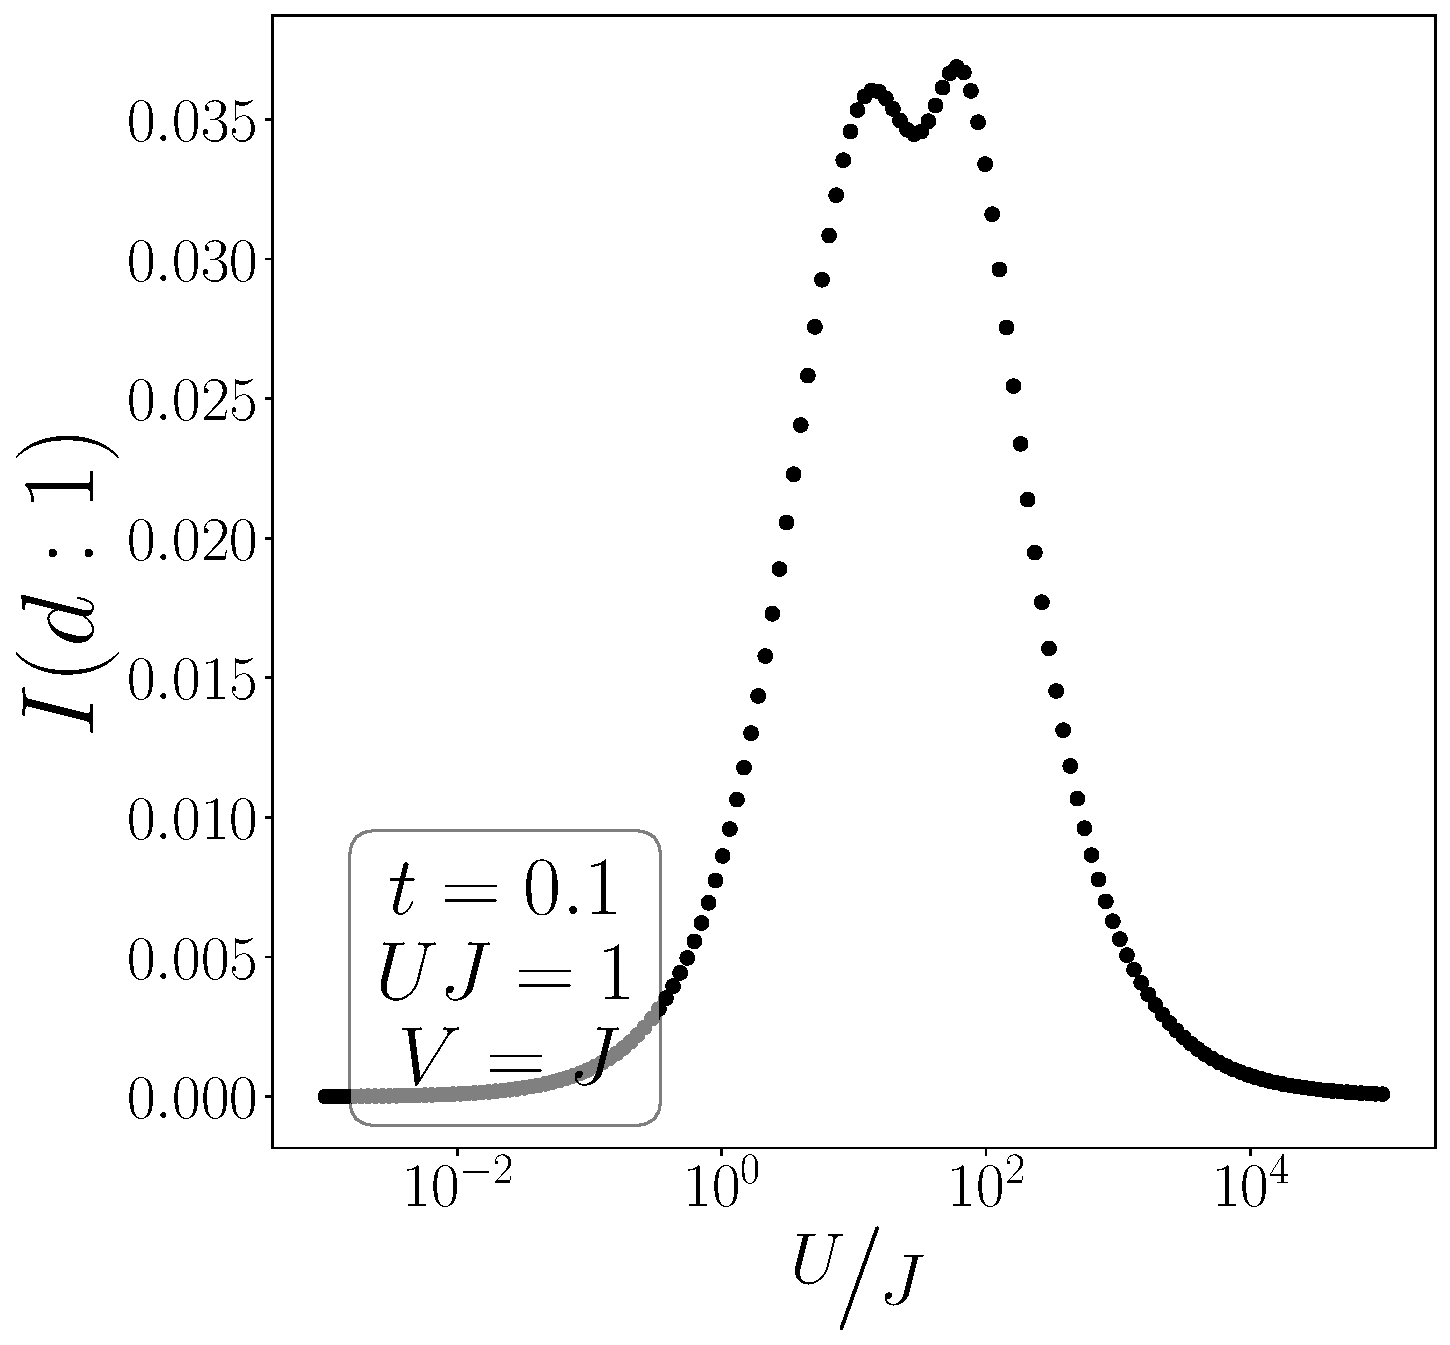
\includegraphics[width=0.32\textwidth]{../figures/mi-d1-t=0.100,J=1_over_U,V=J,N=6,U=0.032,316.228,150.pdf}
	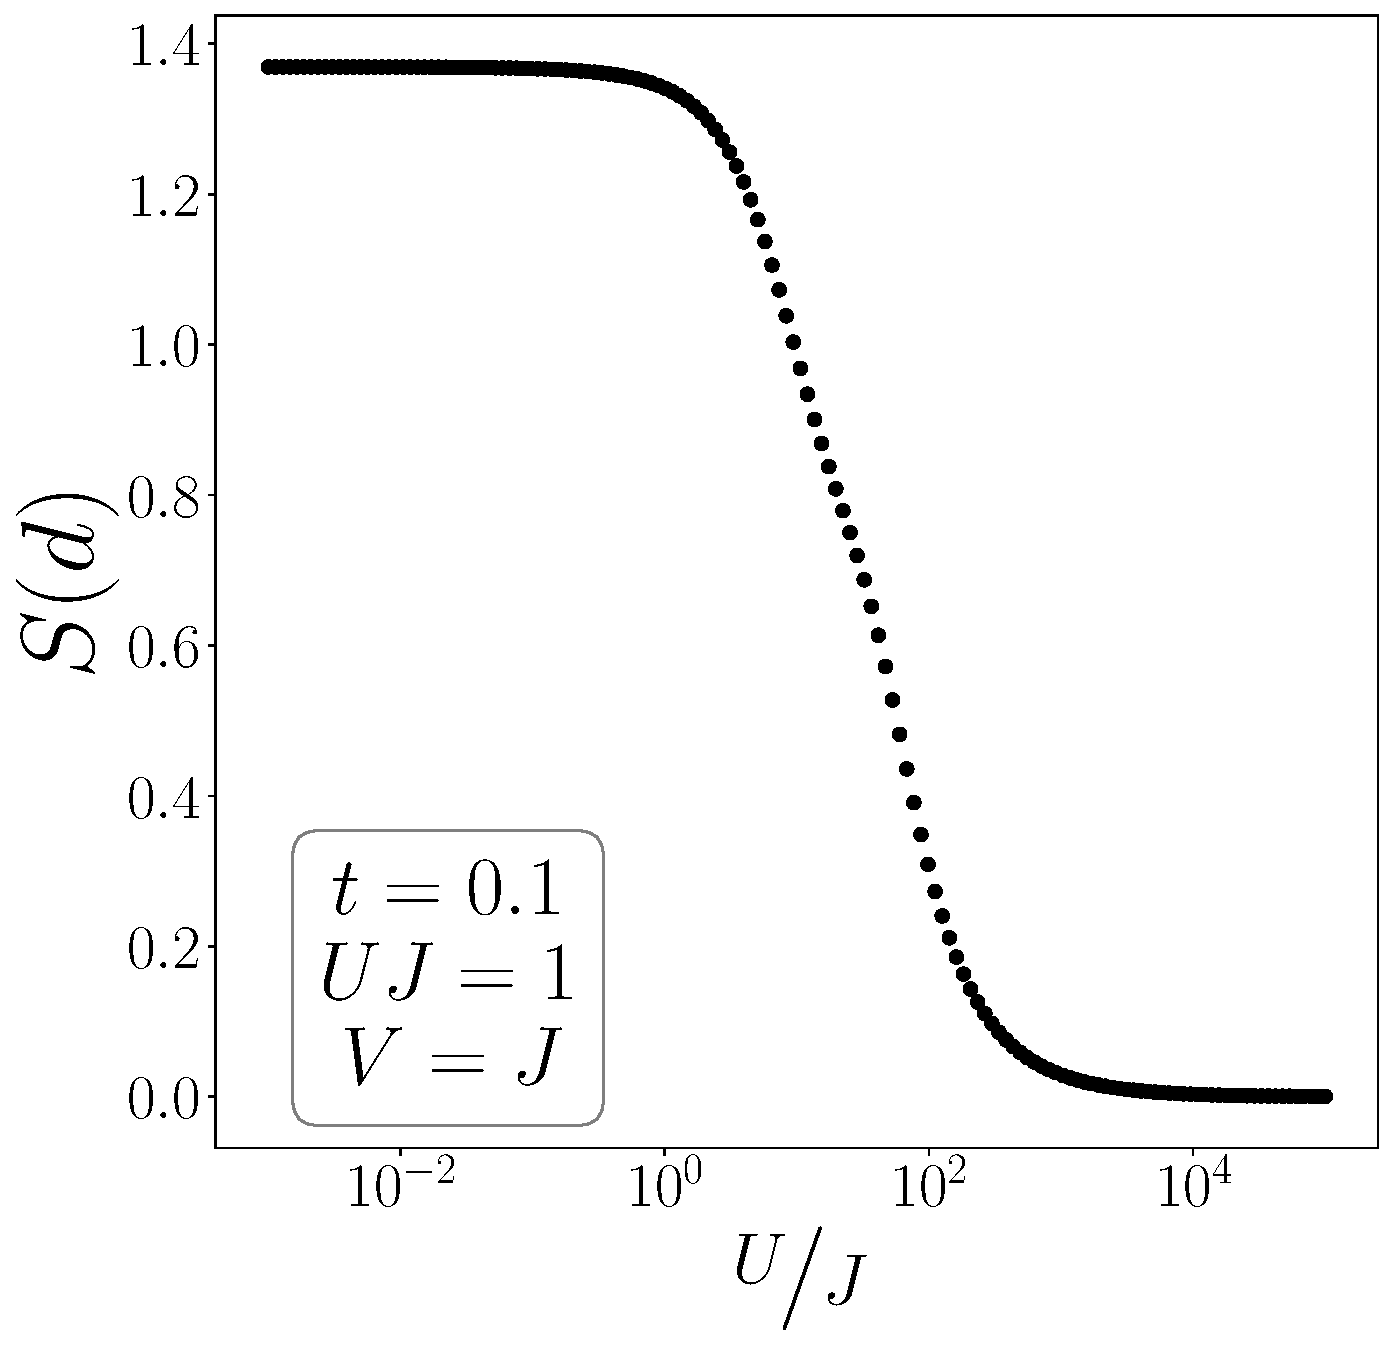
\includegraphics[width=0.32\textwidth]{../figures/EE-d-t=0.100,J=1_over_U,V=J,N=6,U=0.032,316.228,150.pdf}
	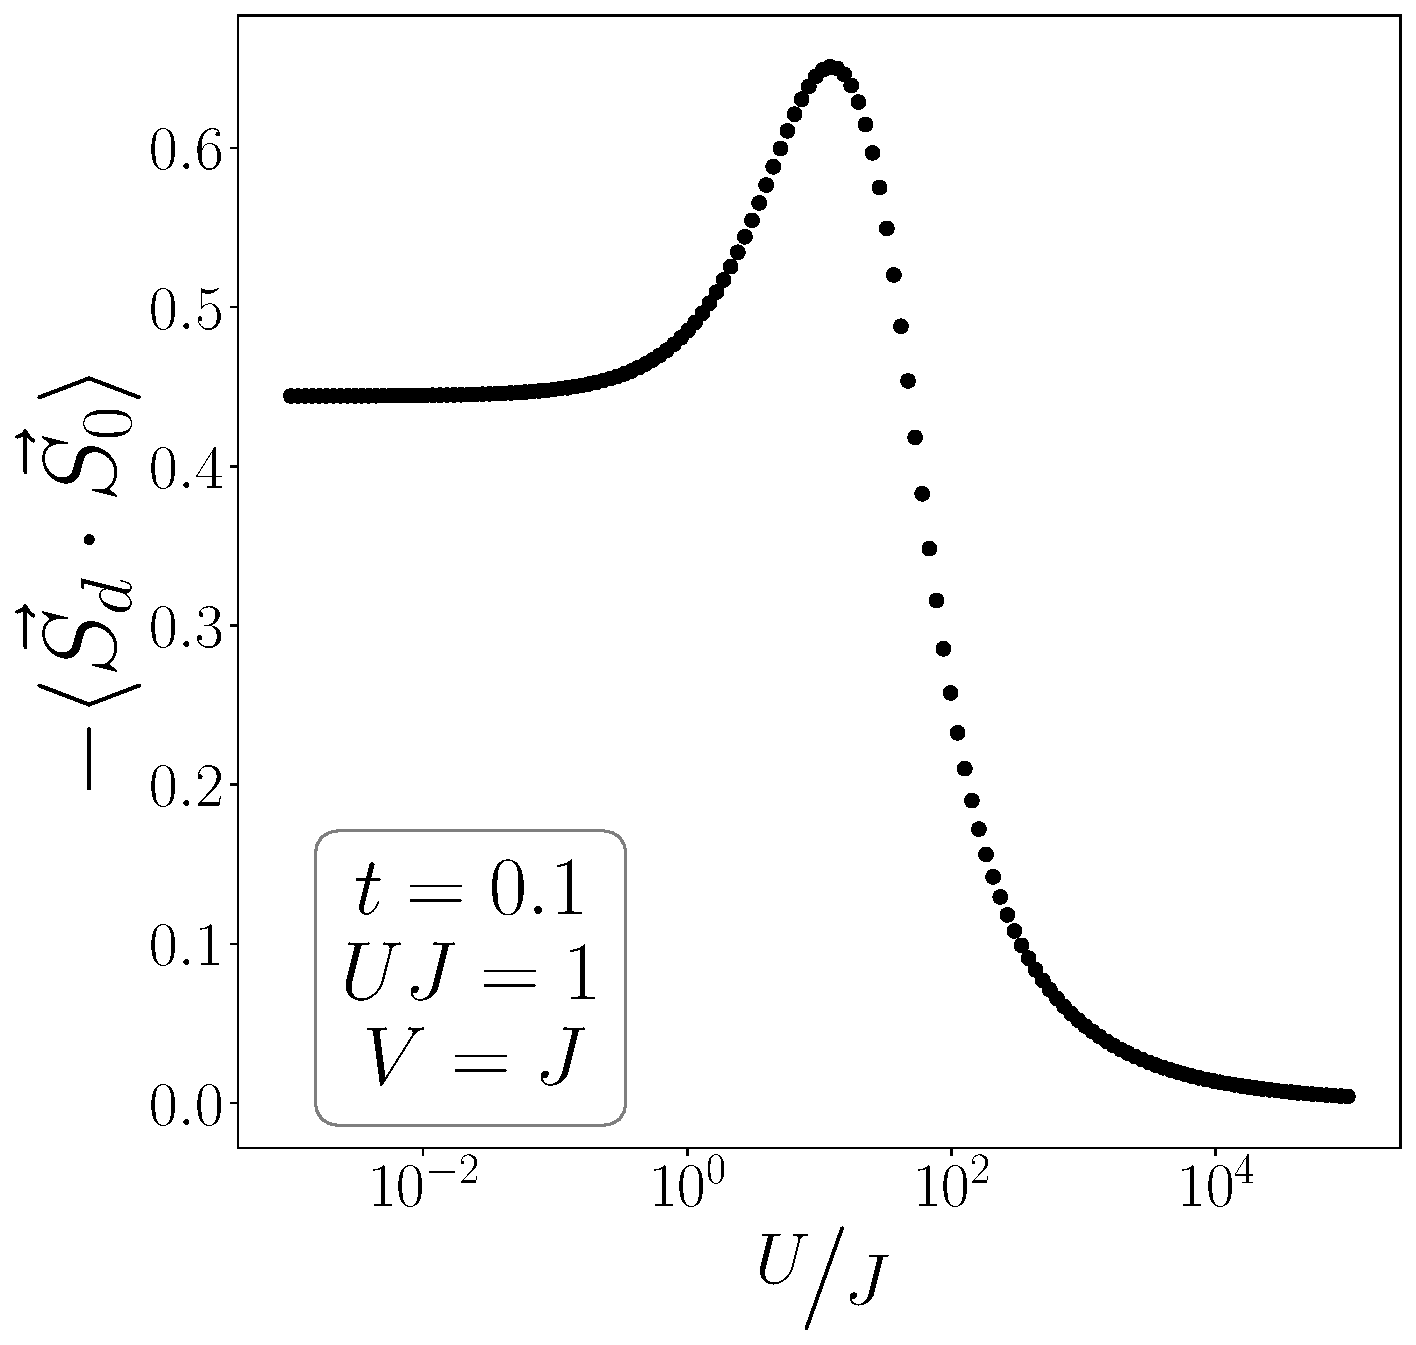
\includegraphics[width=0.32\textwidth]{../figures/corr-d0-t=0.100,J=1_over_U,V=J,N=6,U=0.032,316.228,150.pdf}
	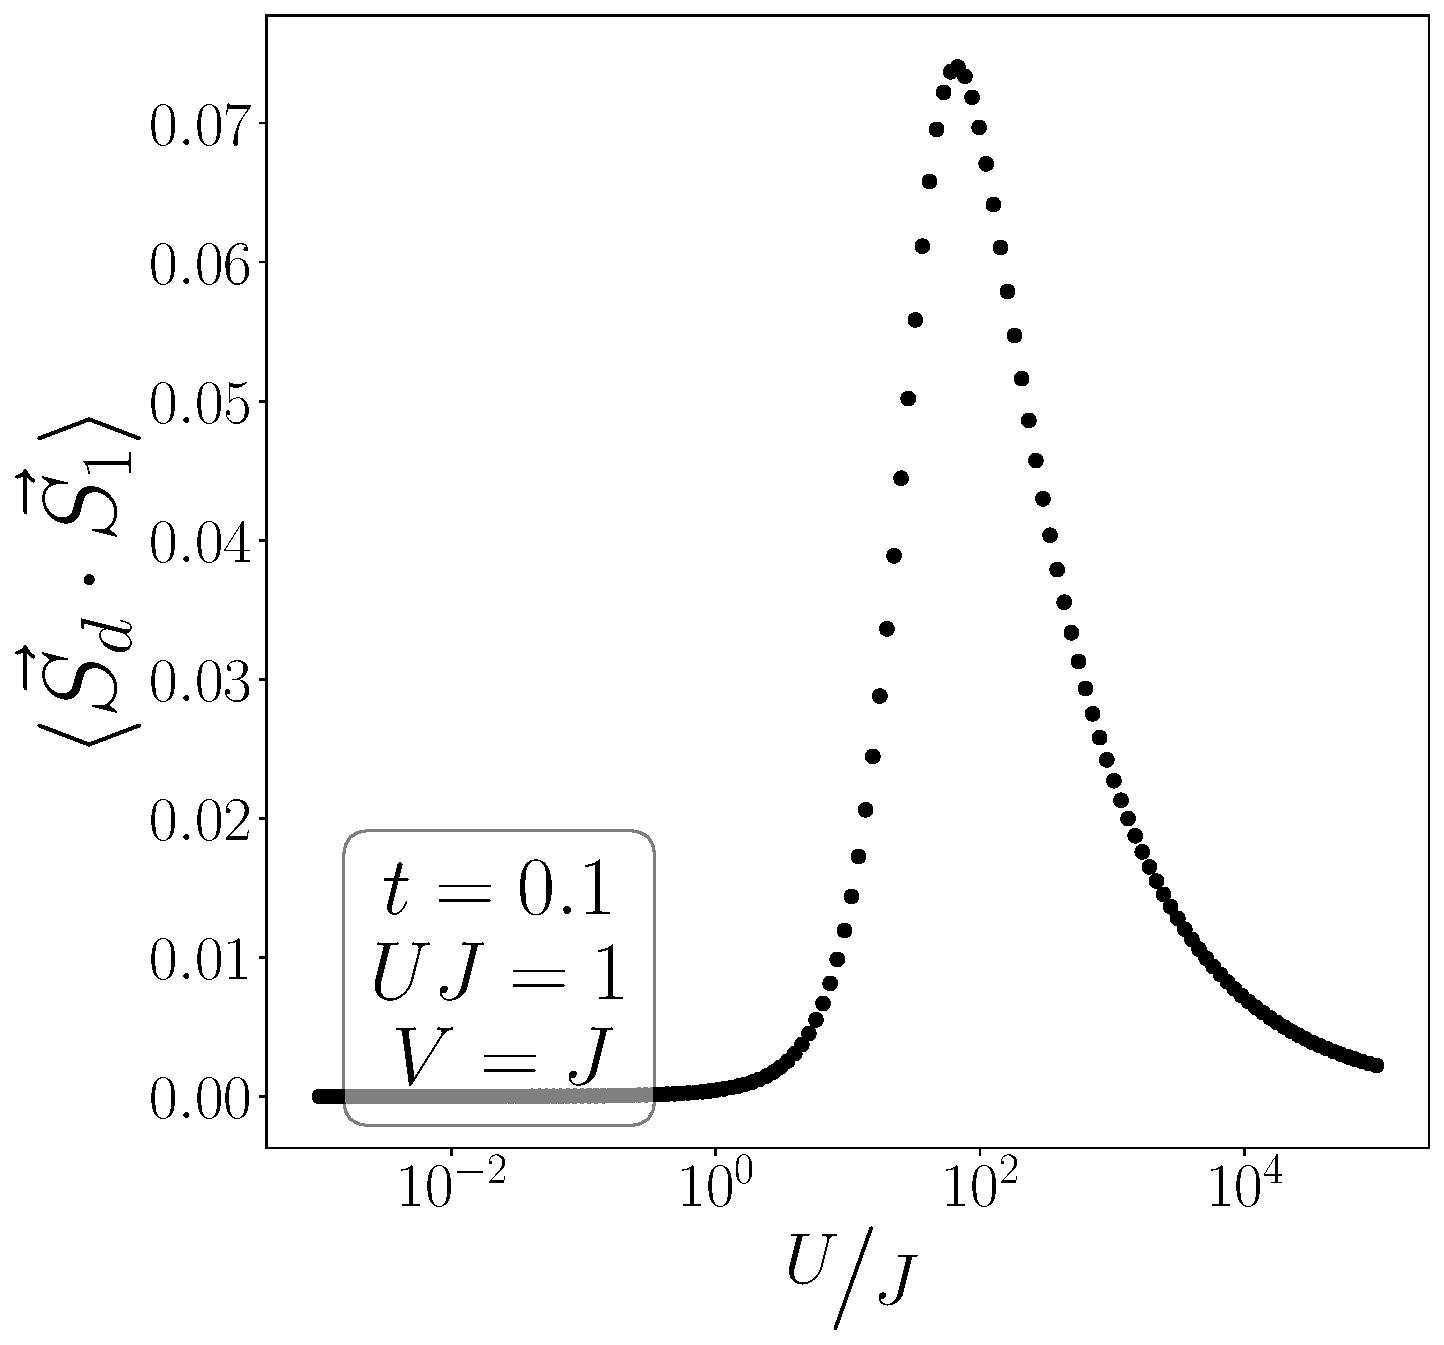
\includegraphics[width=0.32\textwidth]{../figures/corr-d1-t=0.100,J=1_over_U,V=J,N=6,U=0.032,316.228,150.pdf}\\
	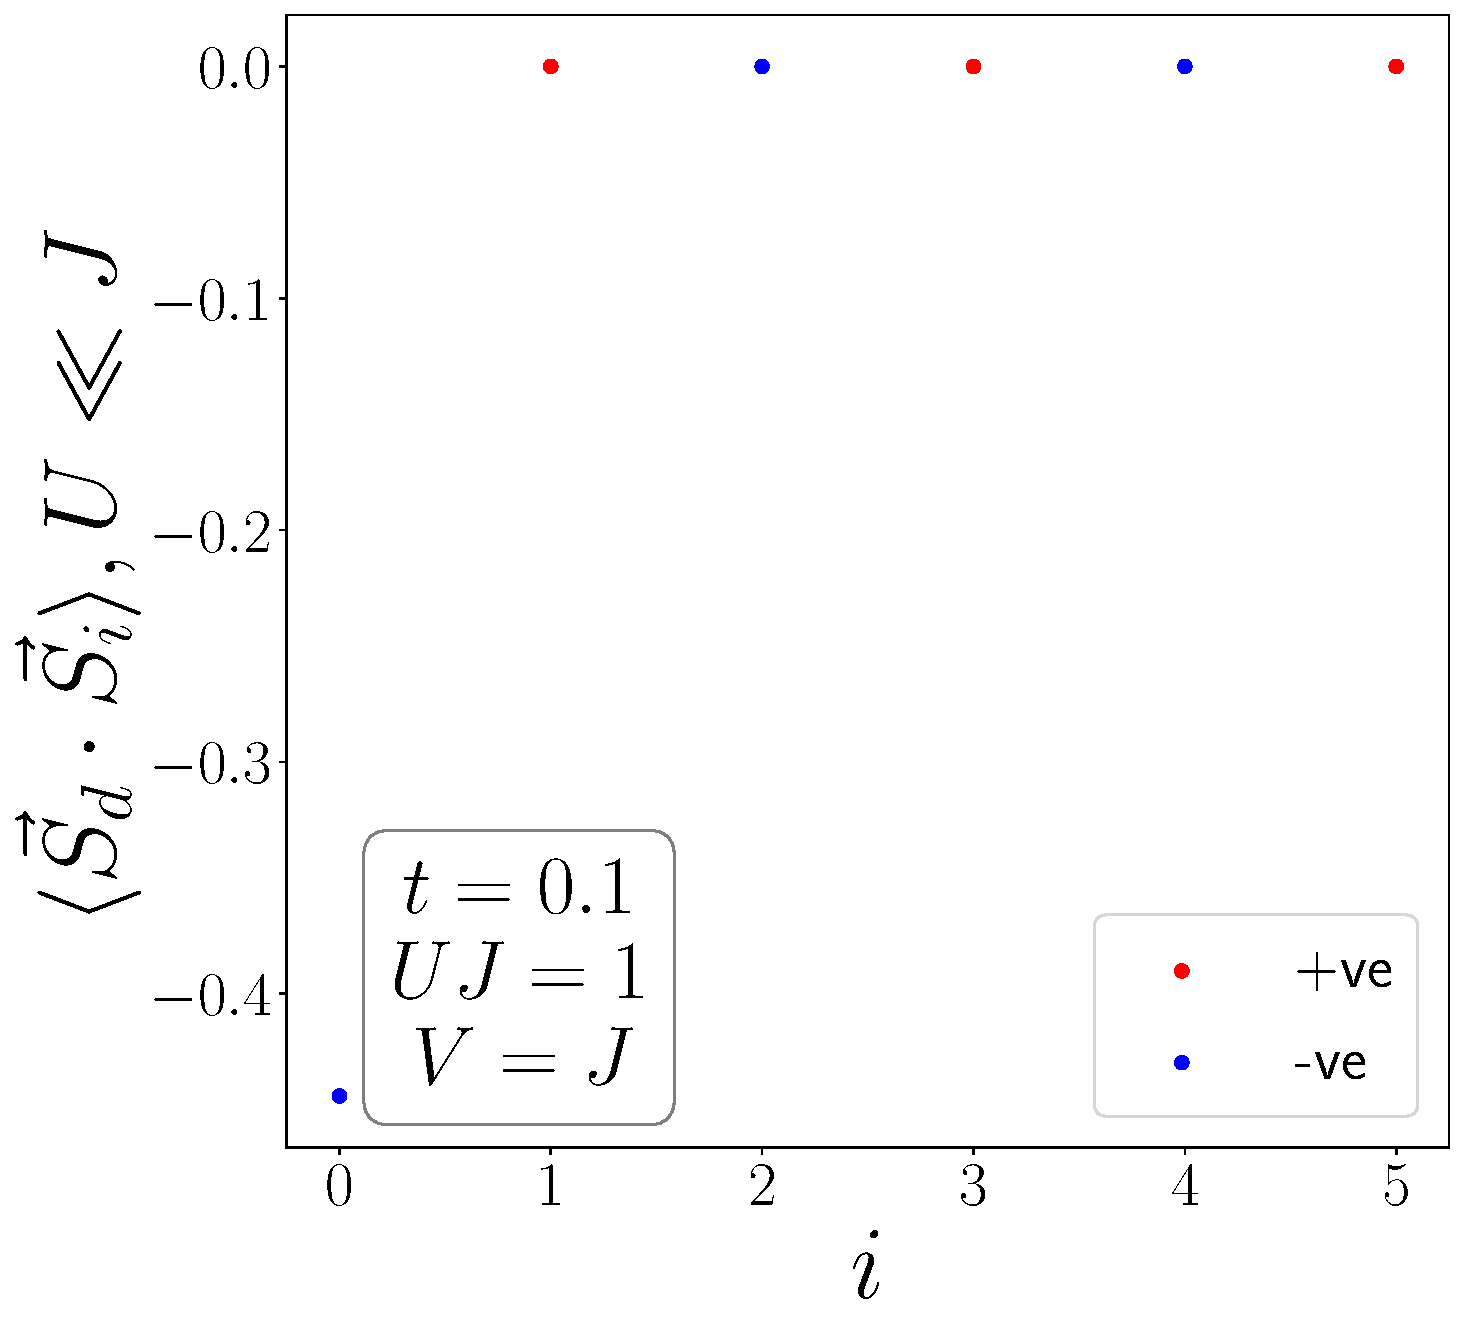
\includegraphics[width=0.32\textwidth]{../figures/corr-di-min-t=0.100,J=1_over_U,V=J,N=6,U=0.032,316.228,150.pdf}
	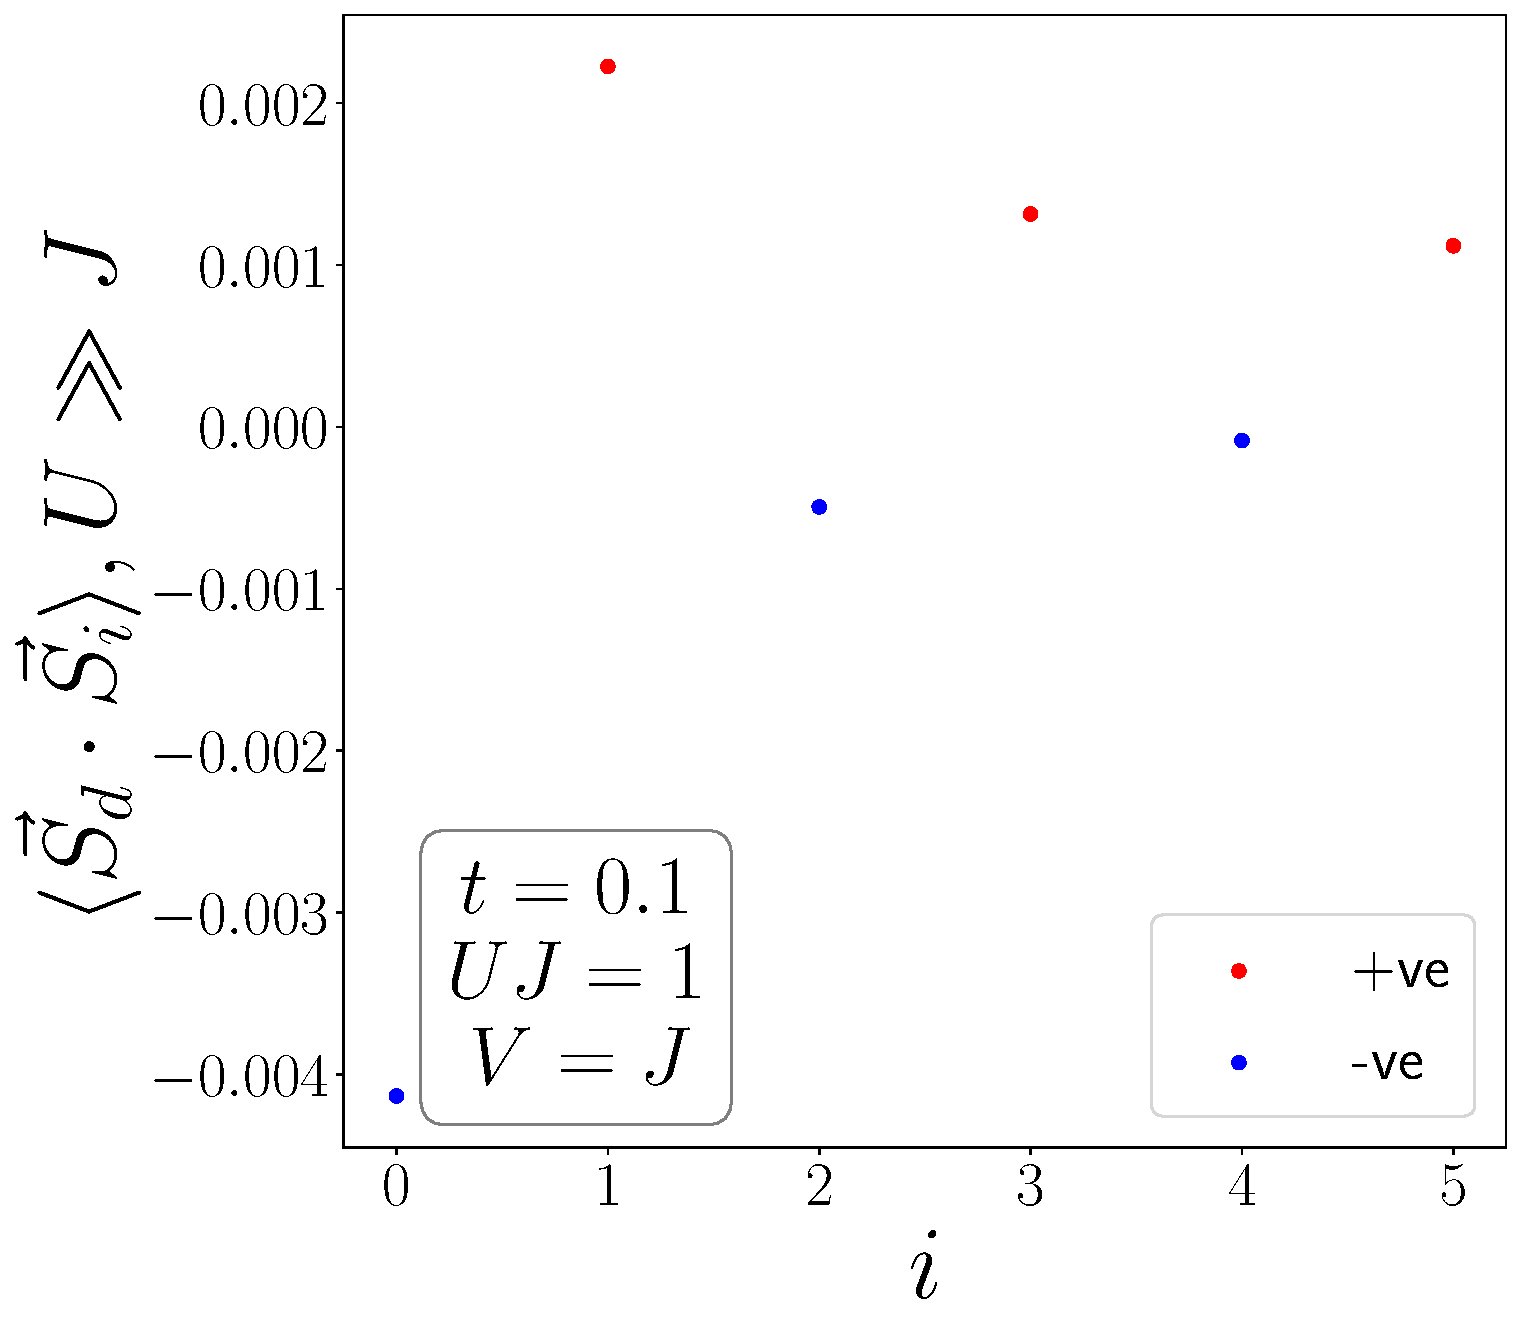
\includegraphics[width=0.32\textwidth]{../figures/corr-di-max-t=0.100,J=1_over_U,V=J,N=6,U=0.032,316.228,150.pdf}
	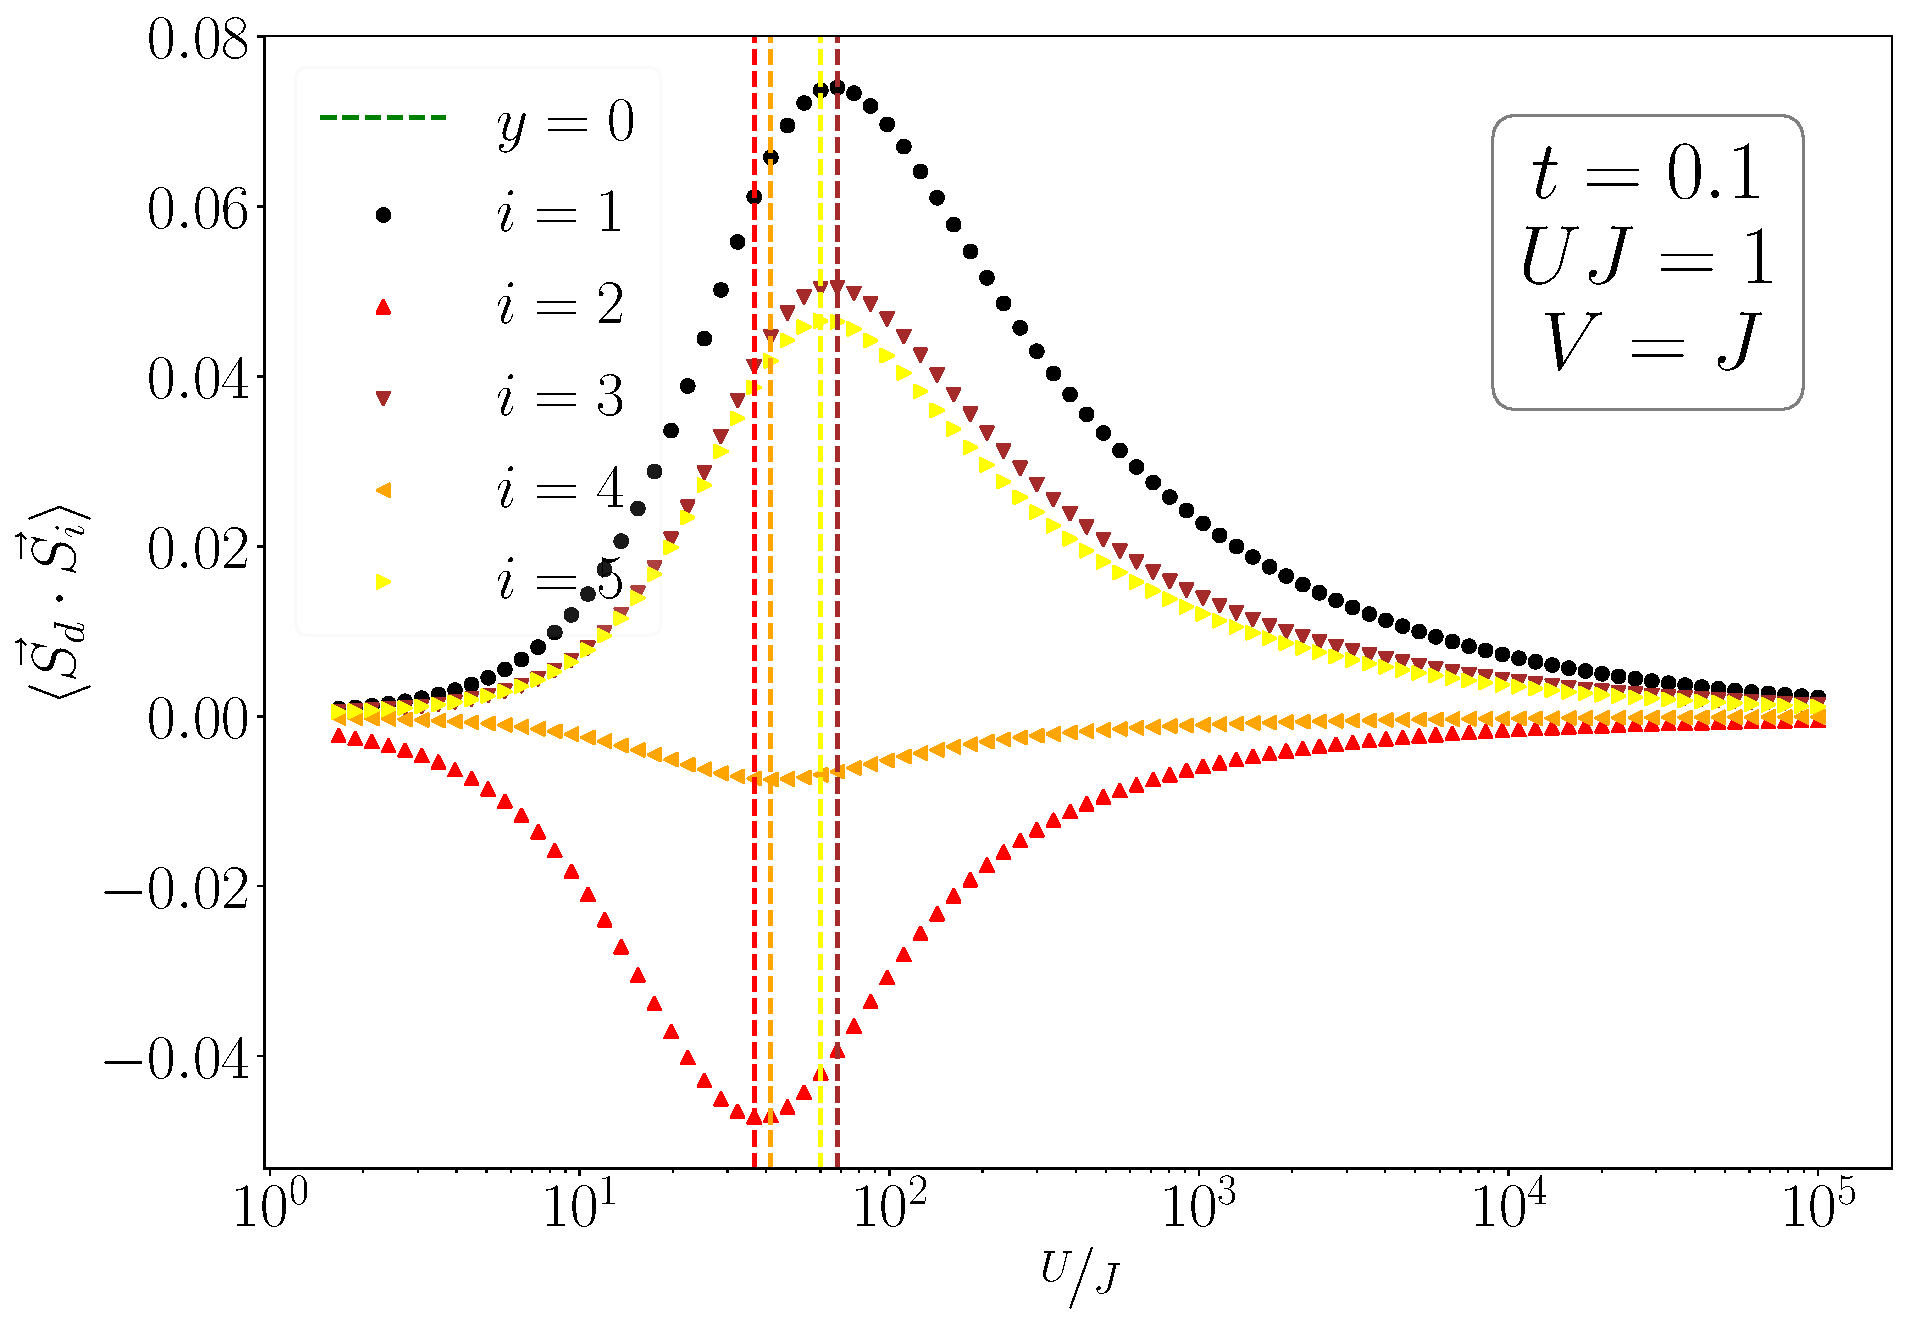
\includegraphics[width=0.6\textwidth]{../figures/corr-all-t=0.100,J=1_over_U,V=J,N=6,U=0.032,316.228,150.pdf}
	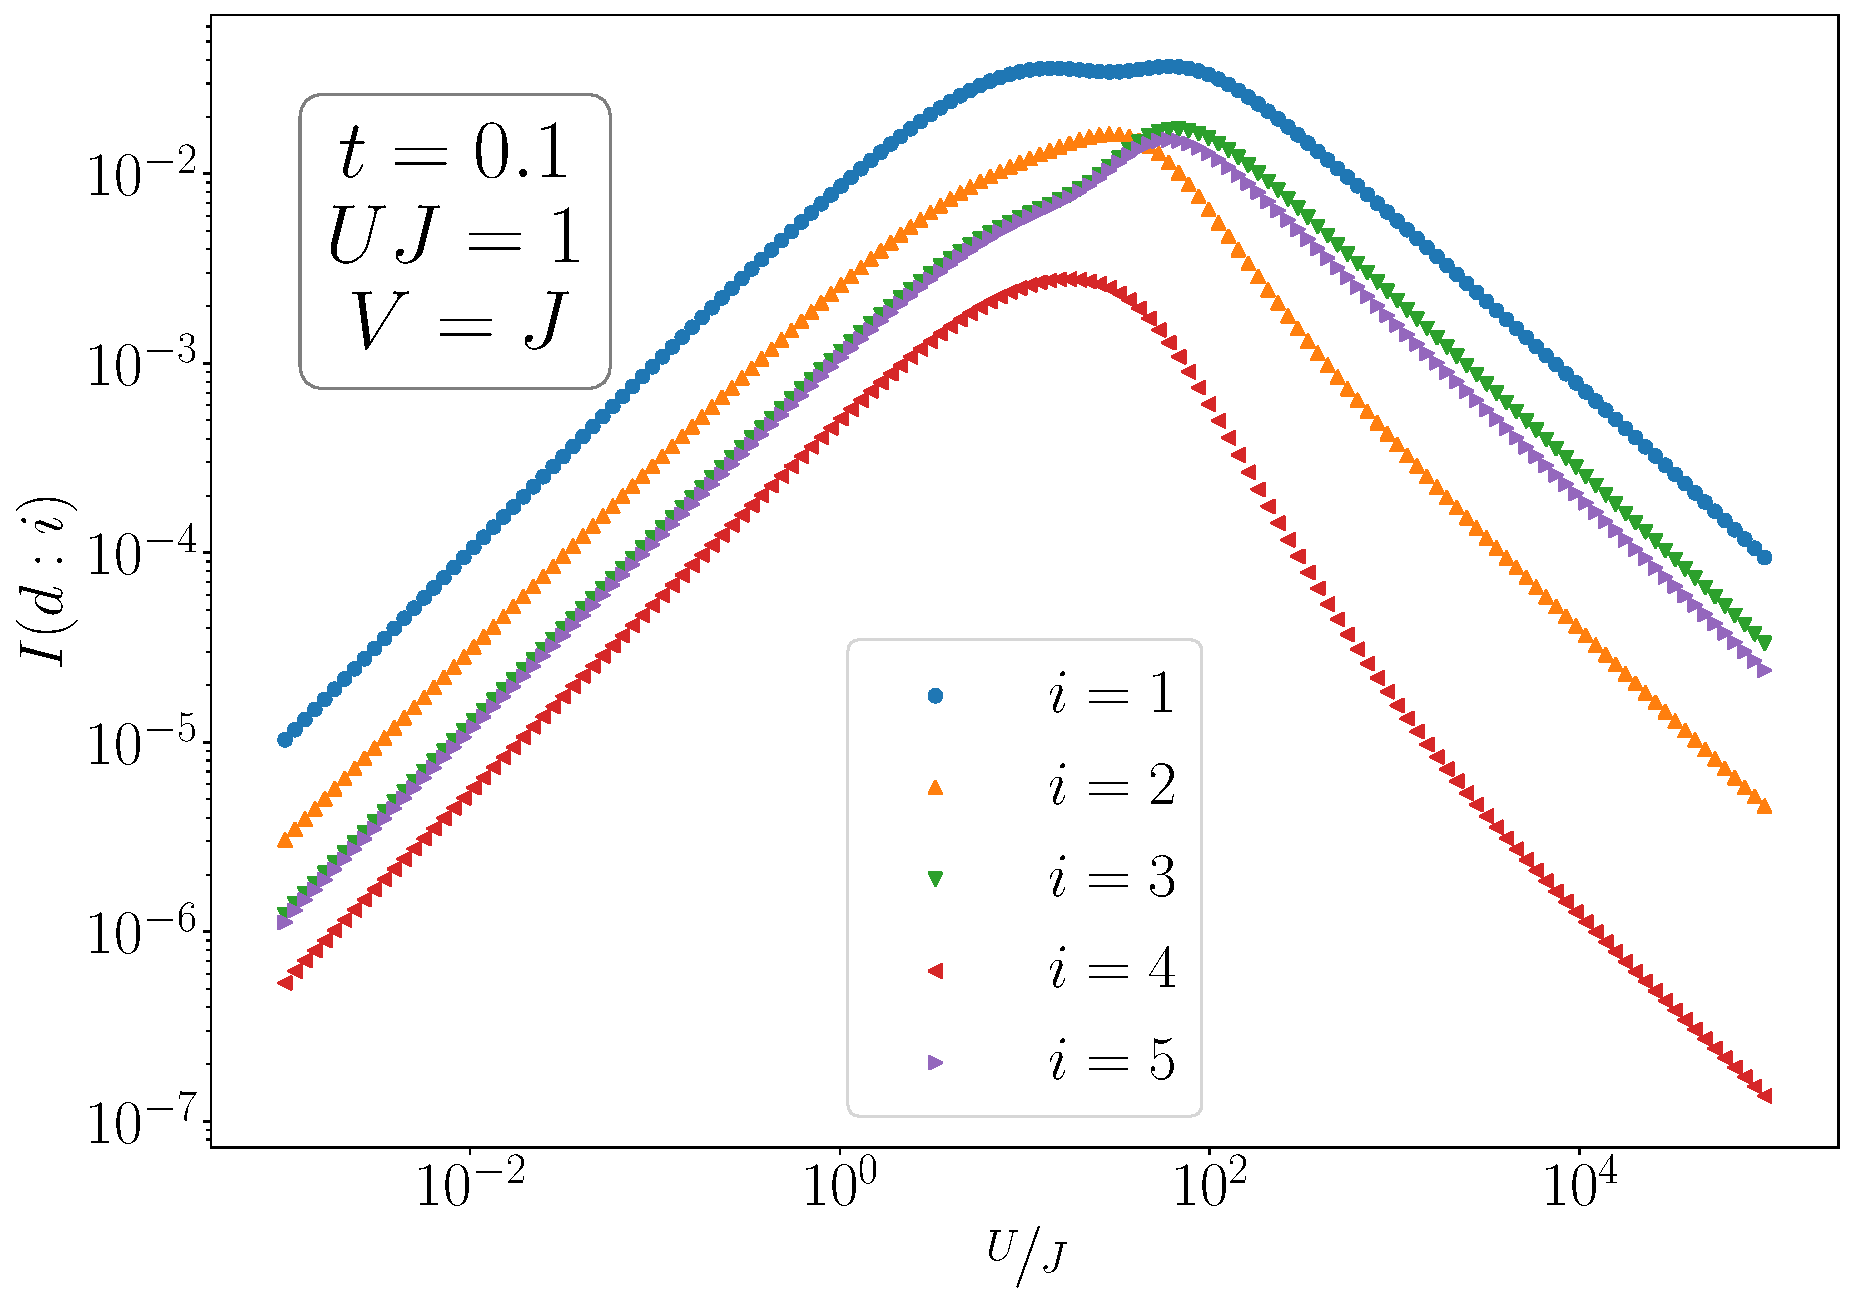
\includegraphics[width=0.6\textwidth]{../figures/I-all-t=0.100,J=1_over_U,V=J,N=6,U=0.032,316.228,150.pdf}
	
\end{center}

\section{Calculating the \(T=0\) Wilson ratio from low energy excitations}
The total system now consists of two decoupled parts - the singlet composed of the impurity and the zeroth site, and the remaining lattice composed of N-1 sites with a tight-binding dispersion and a local interaction at the 1-th site. The effective Hamiltonian for the remaining lattice is
\begin{equation}\begin{aligned}
	\sum_{i=1\atop{\sigma}}^\infty t\left(c^\dagger_{i\sigma}c_{i+1 \sigma} + c^\dagger_{i+1 \sigma}c_{i\sigma}\right) + u \hat n_{1 \uparrow} \hat n_{1 \downarrow}
\end{aligned}\end{equation}
We have rewritten the holon term in terms of the spin and doublon operators.
\begin{figure}[htpb]
	\centering
	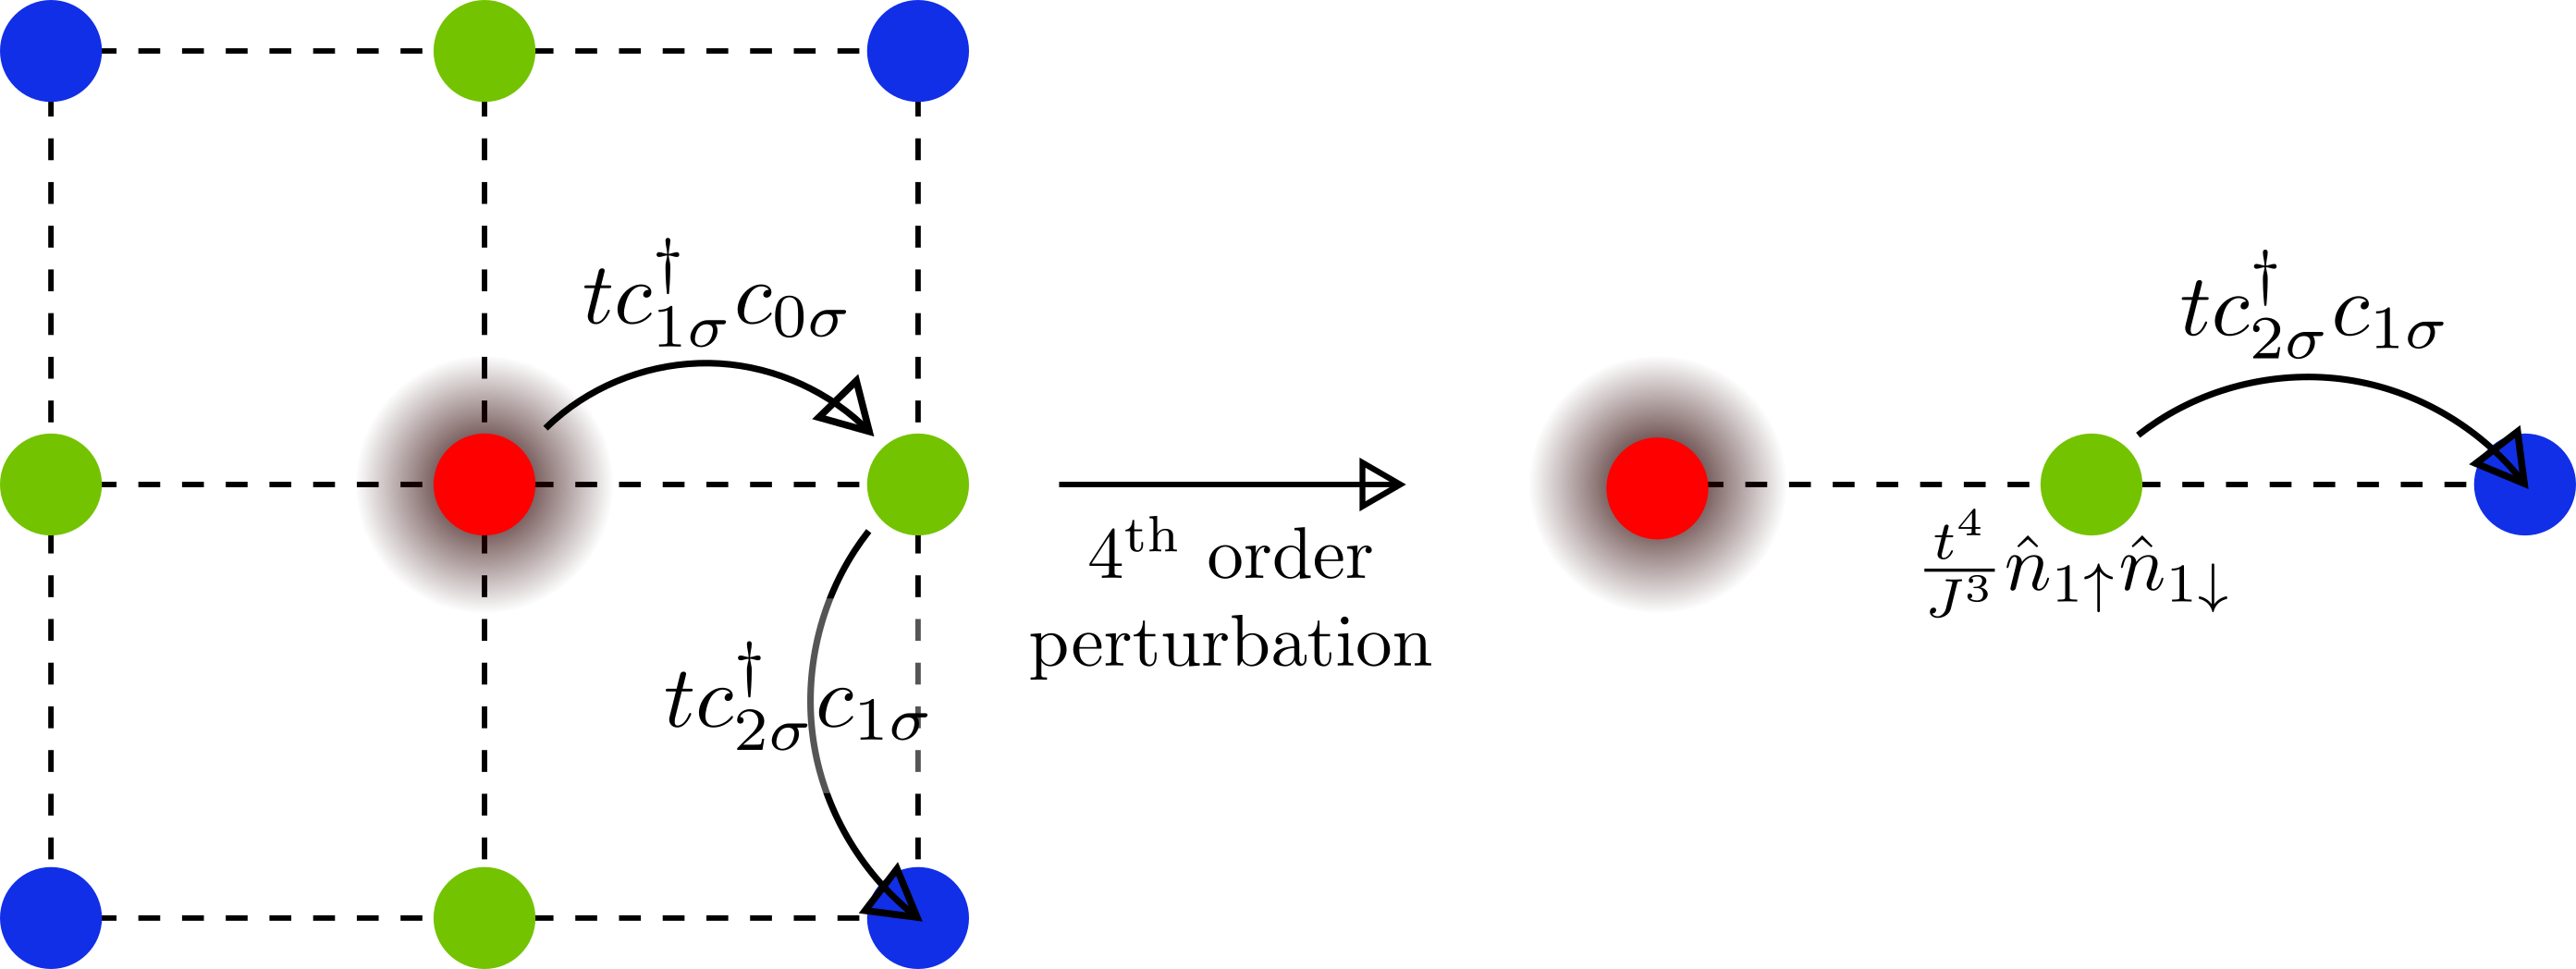
\includegraphics[width=0.7\textwidth]{../figures/lattice_eff.png}
	\caption{\textit{Left}: The nearest-neighbor hopping described by the effective Hamiltonian. The red circle is the impurity. The black cloud at the center demarcates the collection of electrons at the origin of the lattice (which couple to the impurity). The green circles represent lattice sites that are nearest to the origin. The blue circles represent next-nearest sites. \textit{Right}: After treating the hopping between origin and its nearest neighbors as perturbation, we get a system consisting of two decoupled parts: one part is the impurity+cloud singlet, the other part is the rest of the lattice sites. The effect of the hopping between the origin and the green sites is a repulsion term on the green sites.}
\end{figure}
We will now invoke the mean-field approximation in simplifying this term. We will be dealing with thermodynamic quantities soon, so the operators will be replaced by their thermodynamic values, that is, the values that minimize the free energy functional.
\begin{equation}\begin{aligned}
	\hat n_{1 \uparrow} \hat n_{1 \downarrow} \to \langle \hat n_{1 \uparrow} \hat n_{1 \downarrow}\rangle = \langle  \delta n_{1 \uparrow} \delta n_{1 \downarrow}\rangle + \langle  n_{1 \uparrow}\rangle\langle  n_{1 \downarrow}\rangle
\end{aligned}\end{equation}
where \(\delta n_{1\sigma} \equiv n_{1 \sigma} - \langle  n_{1\sigma} \rangle\) is the fluctuation of the particle number above the ground state. The mean-field approximation then involves dropping the first term which is a quadratic fluctuation - since we are interested in values of quantities at \( T \to 0\), this quadratic fluctuation is very small. The interaction we are left with is 
\begin{equation}\begin{aligned}
	u\langle  n_{1 \uparrow}\rangle\langle  n_{1 \downarrow}\rangle = \sum_{kq\sigma}f_{kq}\langle  n_{k \sigma}\rangle\langle  n_{q \overline\sigma}\rangle
\end{aligned}\end{equation}
This interaction converts the problem to that of a Landau Fermi liquid, with the quasiparticle energy functional being given by
\begin{equation}\begin{aligned}
	\epsilon_{k\sigma} = \epsilon_k + \sum_{q}f_{kq}\left<\hat n_{q \overline\sigma}\right>
\end{aligned}\end{equation}
From the form of the quasiparticle energy functional, we can see that there is no spin-parallel term, so we can write
\begin{equation}\begin{aligned}
	\label{rel_landau}
	f_{kk^\prime\sigma\sigma} = 0,  f_{kk^\prime\sigma\overline\sigma} = f_{kk^\prime}
\end{aligned}\end{equation}
We will now use this Fermi liquid form to extract the Wilson ratio. We will make use of the following definitions/results:
\begin{gather}
	dn_{k\sigma} = \frac{\partial{n}}{\partial{\epsilon_{k\sigma}}}\left( d\epsilon_{k\sigma} - d\mu \right) ~ ~ \left[\text{follows from differentiating FD distribution}\right] \\
	C_V = \frac{\:\mathrm{d}\epsilon}{\:\mathrm{d}T}, ~ ~ \chi^{s,c} = \frac{\:\mathrm{d}}{\:\mathrm{d}(B, \mu)}\left(n_\uparrow \mp n_\downarrow\right), ~ ~ 2f_0^{s,a} = \sum_k\left(f_{kk^\prime \uparrow \uparrow} \pm f_{kk^\prime \uparrow \downarrow}\right), ~ ~ F_0^{s,a} = \rho(0) f_0^{s,a}
\end{gather}
\subsection{Low-\(T\) Specific heat}
\begin{equation}\begin{aligned}
	C &= \frac{\:\mathrm{d}}{\:\mathrm{d}T}\sum_{k\sigma}\epsilon_{k\sigma}n_{k\sigma} \\
	    &\approx \sum_{k\sigma}\epsilon^0_{k\sigma} \frac{\:\mathrm{d}n_{k\sigma}}{\:\mathrm{d}T} && \left[\text{no quasiparticles at ground state}\right] \\
	    &\approx \sum_{k\sigma}\epsilon^0_{k\sigma} \frac{\:\mathrm{d}n_{k\sigma}}{\:\mathrm{d}T} && \left[\text{same expression as Fermi gas but with modified distribution function}\right] \\
	    &= \rho(0) T
\end{aligned}\end{equation}
where \(\rho\) is the total quasiparticle DOS with contributions from conduction bath and impurity.
\begin{equation}\begin{aligned}
	\rho \sim \text{Im }\text{Trace}\left[G\right] = \text{Im}\sum_{d\sigma}G_{dd}^\sigma + \text{Im}\sum_{k\sigma}G_{kk}^\sigma = \rho_0 + \rho_\text{imp}
\end{aligned}\end{equation}
which gives
\begin{equation}\begin{aligned}
	C_{imp} \equiv C - C_0 = \rho_{imp}(0)T
\end{aligned}\end{equation}

\subsection{Low-\(T\) Charge Susceptibility}
\begin{equation}\begin{aligned}
	\chi^c &= \frac{\:\mathrm{d}N}{\:\mathrm{d}\mu}\\
\end{aligned}\end{equation}
Due to change in chemical potential, \(\delta\epsilon_{k\sigma}\) is isotropic and SU(2)-symmetric. Hence
\begin{equation}\begin{aligned}
	d\epsilon_{k\sigma} &= \sum_{k^\prime\sigma^\prime}f_{kk^\prime\sigma\sigma^\prime}d n_{k^\prime\sigma^\prime}\\
			    &= d n\sum_{k^\prime}\left(f_{kk^\prime\uparrow \uparrow} + f_{kk^\prime \uparrow \downarrow}\right) && \left[dn = dn_{k^\prime \uparrow} = dn_{k \downarrow}\right] \\
			    &= 2dn f_0^s
\end{aligned}\end{equation}
Therefore,
\begin{equation}\begin{aligned}
	dN &= \sum_{k\sigma}dn_{k\sigma} = \sum_{k\sigma}\frac{\partial{n}}{\partial{\epsilon_{k\sigma}}}\left( d\epsilon_{k\sigma} - d\mu \right) = \sum_{k\sigma}-\frac{1}{2}\rho\left(2dn f_0^s - d\mu \right) = -\rho(0) d N f_0^s + d\mu \rho(0) \\
	   &\approx d\mu \rho(0) - \rho(0) f_0^s d\mu \rho(0) \left[\text{substitute \(dN\) back into itself}\right] \\
	\implies \frac{\:\mathrm{d}N}{\:\mathrm{d}\mu} &= \rho(0)\left( 1 - \rho(0)f_0^s \right) \implies \chi^c_{imp} = \rho(0)_{imp} - \rho(0)f_0^s \\
\end{aligned}\end{equation}
At an intermediate state, we substituted \(dN\) back into itself and kept only the leading order term. This is justified because \(f_{kk^\prime}\) goes as \(\frac{1}{N J}\). At the fixed point and for a thermodynamically large system, both \(J\) and \(N\) are very large, so keeping only the leading order suffices.

From a previous calculation, we know that the charge susceptibility at \(T=0\) is zero (eq.~\eqref{zero_chi_charge}), so we can write down the following relation:
\begin{equation}\begin{aligned}
	\label{fp_constraint}
	f_0^s = \frac{\rho(0)_{imp}}{\rho(0)}
\end{aligned}\end{equation}

\subsection{Low-\(T\) Spin Susceptibility}
\begin{equation}\begin{aligned}
	\chi^s &= \frac{\:\mathrm{d}m}{\:\mathrm{d}\mu}\\
\end{aligned}\end{equation}
Due to change in magnetic field, change in \(\epsilon_{k\sigma}\) should be isotropic and SU(2)-\text{anti}symmetric. Hence
\begin{equation}\begin{aligned}
	d\epsilon_{k\sigma} &= -\frac{1}{2}dB \sigma + \sum_{k^\prime\sigma^\prime}f_{kk^\prime\sigma\sigma^\prime}d n_{k^\prime\sigma^\prime}\\
			    &= -\frac{1}{2}dB \sigma + d n_{\sigma}\sum_{k^\prime}\left(f_{kk^\prime\uparrow \uparrow} - f_{kk^\prime \uparrow \downarrow}\right) && \left[dn_{k^\prime \uparrow} = -dn_{k \downarrow}\right] \\
			    &= -\frac{1}{2}dB \sigma + 2dn_\sigma f_0^a
\end{aligned}\end{equation}
Since the total number remains constant, \(\mu=0\). Therefore,
\begin{equation}\begin{aligned}
	dm &= \sum_{k}\left(dn_{k \uparrow} - dn_{k \downarrow}\right) = -\frac{1}{2}\sum_{k}\rho\left( d\epsilon_{k \uparrow} - d\epsilon_{k \downarrow} \right) = -\frac{1}{2}\sum_{k}\rho\left(-dB + 2f_0^a \left(dn_{k \uparrow} - dn_{k \downarrow}\right)\right) \\
	   &= dB\rho(0) - dm \rho(0)f_0^a \approx dB\rho(0) - \rho(0)f_0^aB\rho(0) ~ \left[\text{substitute \(dm\) back into itself}\right] \\
	\implies \frac{\:\mathrm{d}m}{\:\mathrm{d}B} &= \rho(0)\left( 1 - \rho(0)f_0^a \right) \implies \chi^s_{imp} = \rho(0)_{imp} - \rho(0)f_0^a \\
\end{aligned}\end{equation}

\subsection{Wilson ratio}
The Wilson ratio for the impurity is defined as
\begin{equation}\begin{aligned}
	R = \frac{\chi^s_{imp}}{\frac{C_{imp}}{T}}
\end{aligned}\end{equation}
From eq.~\eqref{rel_landau}, we have \(f_0^s = -f_0^a\), which, when combined with eq.~\eqref{fp_constraint}, gives
\begin{equation}\begin{aligned}
	\chi^s_{imp} &= 2\rho(0)_{imp}
\end{aligned}\end{equation}
The Wilson ratio becomes
\begin{equation}\begin{aligned}
	R = \frac{2\rho(0)_{imp}}{\rho(0)_{imp}} = 2
\end{aligned}\end{equation}

\section{Luttinger's and Friedel's sum rules}
The subsequent discussions are for the first quadrant where \(U^* = 0\) and \(J^* > K^*\). At high temperatures, we see that the impurity susceptibility attains the value of
\begin{equation}\begin{aligned}
	\frac{1}{8k_B T}
\end{aligned}\end{equation}
which implies that the impurity behaves as a free orbital in this limit, having no coupling with the bath. We can write down the following effective Hamiltonian for such a limit:
\begin{equation}\begin{aligned}
	\mathcal{H}_\text{high-T} = \tilde \epsilon_d \hat n_d + \sum_{k\sigma} \epsilon_k\hat n_{k\sigma}
\end{aligned}\end{equation}
Since the impurity is decoupled from the bath, we can immediately write down the Hamiltonian just for the impurity:
\begin{equation}\begin{aligned}
	\mathcal{H}_\text{high-T, imp} = \tilde \epsilon_d \hat n_d
\end{aligned}\end{equation}

We consider the resonant-level model:
\begin{equation}\begin{aligned}
	\mathcal{H}_\text{res} = \sum_{k\sigma}\epsilon_k \hat n_{k\sigma} + \epsilon_d n_d + \sum_{k\sigma}\left(V_k c^\dagger_{k\sigma} c_{d\sigma} + \text{h.c.}\right)
\end{aligned}\end{equation}
The total Green's function is 
\begin{equation}\begin{aligned}
	G(z) = \frac{1}{z - \mathcal{H}_\text{res}}
\end{aligned}\end{equation}
The impurity diagonal Green's function is
\begin{equation}\begin{aligned}
	G_{dd}(z) &= \frac{1}{z - \epsilon_d - \Sigma_d(z)}, &&	G_d(z) = G_{dd}\ket{d}\bra{d}
\end{aligned}\end{equation}
where \(\Sigma_d(z)\) is in general complex and is zero at the free orbital fixed point. The conduction electron Green's function is 
\begin{equation}\begin{aligned}
	&G_{kk}(z) = G_k^0(z) + \left[G_k^0(z)V_k\right]^2 G_{dd}(z), & G_c(z) \equiv \sum_k \ket{k}\bra{k}G_{kk}(z), && G_{c0}(z) \equiv \sum_k G_{kk}^0(z)\ket{k}\bra{k}
\end{aligned}\end{equation}
The total Green's function can be written as
\begin{equation}\begin{aligned}
	G(z) &= \left(\sum_{k}\ket{k}\bra{k} + \ket{d}\bra{d}\right) G \left(\sum_{k}\ket{k}\bra{k} + \ket{d}\bra{d}\right)\\
	     &= \sum_{k} \ket{k}\bra{k}G_{kk}(z) + G_{dd}(z)\ket{d}\bra{d} + \text{off-diagonal terms}\\
	     &= G_c(z) + G_{d}(z) + \text{off-diagonal terms}
\end{aligned}\end{equation}
The total number of electrons is given by
\begin{equation}\begin{aligned}
	N &= \oint \frac{dz}{2\pi i}n_F(z) \text{Tr}\left[G(z) \right]\\
	  &= \oint \frac{dz}{2\pi i}n_F(z) \text{Tr}\left[G_{d}(z) + G_c(z)\right]
\end{aligned}\end{equation}
The contour \(\Gamma\) counts all the singularities of \(\text{Tr} G(z)\), and thus encloses only the real axis of the complex plane (since \(G(z)\) comes from a Hermitian matrix \(\mathcal{H}_\text{res}\), all its singularities are real).
At this point, we can use an identity:
\begin{equation}\begin{aligned}
	\text{Tr}\left[G_{d}(z)\right] &= \text{Tr}\left[ \frac{\ket{d}\bra{d}}{z - \epsilon_d - \Sigma_d(z)}\right] = \text{Tr}\left[ \frac{\ket{d}\bra{d}}{z - \epsilon_d - \Sigma_d(z)}\frac{\partial{\left(z - \epsilon_d\right)}}{\partial{z}} \right] = \text{Tr}\left[ \ket{d}\bra{d}G_{dd}\frac{\partial{\left\{G_{dd}^{-1}(z) + \Sigma_d(z)\right\}}}{\partial{z}} \right]\\
				       &= \text{Tr}\left[ G_{d}(z)\frac{\partial{G_{d}^{-1}(z)}}{\partial{z}} \right] + \text{Tr}\left[ G_{d}(z)\frac{\partial{\Sigma_d(z)}}{\partial{z}} \right] = \frac{\partial{}}{\partial{z}}\left[\ln \text{Det}G_{d}^{-1}(z)\right] + \text{Tr}\left[ G_{d}(z)\frac{\partial{\Sigma_d(z)}}{\partial{z}} \right]\\
\end{aligned}\end{equation}
In the last step, we converted the trace to a determinant using
\begin{equation}\begin{aligned}
	\text{Tr}\left[A \frac{\partial{A^{-1}}}{\partial{z}}\right] = \frac{\partial{}}{\partial{z}}\text{Tr}\ln A^{-1} =\frac{\partial{}}{\partial{z}}\sum_i \ln \lambda_i = \frac{\partial{}}{\partial{z}}\ln \prod_i \lambda_i = \frac{\partial{}}{\partial{z}}\ln \text{Det}A^{-1}
\end{aligned}\end{equation}
where \(\lambda_i\) are the eigenvalues of \(A^{-1}\). Substituting \(\text{Tr}\left[G_d(z)\right] \) into the total number of particles gives
\begin{equation}\begin{aligned}
	N  &= \oint \frac{dz}{2\pi i}n_F(z) \left[\frac{\partial{}}{\partial{z}} \ln \text{Det} \left\{G^{-1}_d(z)\right\} + \text{Tr} \left( G_d(z) \frac{\partial{}}{\partial{z}}\Sigma_d(z) \right) + \text{Tr}G_c(z)\right]
\end{aligned}\end{equation}
The conduction electron part can also be simplified:
\begin{equation}\begin{aligned}
	\text{Tr}G_c(z) &= \text{Tr}\left[G_{c0}(z) + \sum_k \left\{G_k^0(z)V_k\right\}^2 G_{dd}(z)\ket{k}\bra{k}\right] =\text{Tr}\left[G_{c0}(z)\right] + \sum_k\left[G_k^0(z)V_k\right]^2 G_{dd}(z)\\
\end{aligned}\end{equation}
Since \(G_{c0}^{-1}(z) = z - \sum_k \epsilon_k \hat n_k\), we can write \(\text{Tr}\left[G_{c0}(z)\right] = \text{Tr}\left[G_{c0}(z) \frac{\partial{}}{\partial{z}}G_{c0}^{-1}\right]\) and hence
\begin{equation}\begin{aligned}
	\text{Tr}G_c(z) &=\frac{\partial{}}{\partial{z}}\left[\ln \text{Det}G_{c0}^{-1}(z)\right] + \sum_k\left[G_k^0(z)V_k\right]^2 G_{dd}(z)
\end{aligned}\end{equation}
Updating the total particles with this leads to
\begin{equation}\begin{aligned}
	N  = \oint \frac{dz}{2\pi i}n_F(z) \left[\frac{\partial{}}{\partial{z}} \ln \text{Det} \left\{G^{-1}_d(z)\right\} + \frac{\partial{}}{\partial{z}} \ln \text{Det} \left\{G^{-1}_{c0}(z)\right\} + \text{Tr} \left( G_d(z) \frac{\partial{}}{\partial{z}}\Sigma_d(z) \right) + \sum_k\left( V_k G_k^0 \right)^2 G_{dd}(z)\right]
\end{aligned}\end{equation}
For the resonant-level model, we have
\begin{equation}\begin{aligned}
	\Sigma_d = \sum_k V^2_k G^0_k = \sum_k \frac{V_k^2}{z - \epsilon_k}
\end{aligned}\end{equation}
such that
\begin{equation}\begin{aligned}
	\text{Tr} \left( G_d(z) \frac{\partial{}}{\partial{z}}\Sigma_d(z) \right) = -G_{dd}(z) \sum_k \left( V_k G_k^0 \right)^2
\end{aligned}\end{equation}
which allows us to write
\begin{equation}\begin{aligned}
	N  = \oint \frac{dz}{2\pi i}n_F(z) \left[\frac{\partial{}}{\partial{z}} \ln \text{Det} \left\{G^{-1}_d(z)\right\} + \frac{\partial{}}{\partial{z}} \ln \text{Det} \left\{G^{-1}_{c0}(z)\right\} \right]
\end{aligned}\end{equation}
At \(T=0\), \(n_F\) is defined as 1 below the FS, \(\frac{1}{2}\) at the FS and 0 above it.
\begin{equation}\begin{aligned}
	N  = \left[\oint_{\Gamma_<} + \frac{1}{2}\oint_{\Gamma_0}\right]\frac{dz}{2\pi i}\left[\frac{\partial{}}{\partial{z}} \ln \text{Det} \left\{G^{-1}_d(z)\right\} + \frac{\partial{}}{\partial{z}} \ln \text{Det} \left\{G^{-1}_{c0}(z)\right\} \right]
\end{aligned}\end{equation}
Following Seki and Yunoki, we can define a winding number for a Green's function \(G(z)\):
\begin{equation}\begin{aligned}
	n_{\text{Det} G^{-1}}(C) = \oint_{C} \frac{dz}{2\pi i} \frac{\partial{\ln\text{Det }G^{-1}(z)}}{\partial{z}} = \oint_{\text{Det} G^{-1}(C)} \frac{\mathrm{d}\; \text{Det }G^{-1}}{\text{Det }G^{-1}}
\end{aligned}\end{equation}
Since \(n_{\text{Det } G^{-1}(C)}\) counts the number of times the curve \(\text{Det } G^{-1}(C)\) winds around the origin, it is integer-valued and topological. Seki and Yunoki also show that the this number is given by
\begin{equation}\begin{aligned}
n_{\text{Det }G^{-1}(C)} = P_{\text{Det }G}(C) - Z_{\text{Det }G}(C)
\end{aligned}\end{equation}
where \(P_{f(z)}(C)\) is the number of poles of \(f(z)\) enclosed by the contour \(C\), and \(Z\) is the corresponding number of zeros. The total number of particles in the resonant level model can thus be written as
\begin{equation}\begin{aligned}
	N = P_{\text{Det }G_d}(\Gamma_<) - Z_{\text{Det }G_d}(\Gamma_<) + \frac{1}{2}\left[P_{\text{Det }G_d}(\Gamma_0) - Z_{\text{Det }G_d}(\Gamma_0)\right] + P_{\text{Det }G_{c0}}(\Gamma_<) - Z_{\text{Det }G_{c0}}(\Gamma_<) \\
	+ \frac{1}{2}\left[P_{\text{Det }G_{c0}}(\Gamma_0) - Z_{\text{Det }G_{c0}}(\Gamma_0)\right]
\end{aligned}\end{equation}
The average number of particles can thus be expressed purely in terms of the number of poles and zeros of the impurity and the conduction electron Green's functions. As shown by Seki and Yunoki, the second line gives the Luttinger volume \(V_L\):
\begin{equation}\begin{aligned}
	\label{total_lutt}
	N = P_{\text{Det }G_d}(\Gamma_<) - Z_{\text{Det }G_d}(\Gamma_<) + \frac{1}{2}\left[P_{\text{Det }G_d}(\Gamma_0) - Z_{\text{Det }G_d}(\Gamma_0)\right] + V_L
\end{aligned}\end{equation}
If we start from a non-interacting model (\(V_k = 0\)), we can write
\begin{equation}\begin{aligned}
	N = \mathcal{N}^0_{imp} + V_L^0
\end{aligned}\end{equation}
where \(\mathcal{N}^0_{imp}\) is simply the number of singularities of \(G_d\) on the real axis, for the non-interacting case. We now turn up the interaction \(V_k\), keeping the total number of particles conserved at \(N\). With a non-zero \(V_k\), the impurity self-energy can be written (assuming a constant density of states) as
\begin{equation}\begin{aligned}
	\Sigma_d(z) = \Sigma_d^\text{real}(z) - i \Delta
\end{aligned}\end{equation}
so that the impurity Greens function becomes
\begin{equation}\begin{aligned}
	G_d(z) = \frac{1}{z - \epsilon_d - \Sigma_d^\text{real}(z) + i \Delta}
\end{aligned}\end{equation}
We can see that the presence of an imaginary part lifts the pole of \(G_d(z)\) off the real axis, and since the contour \(\Gamma_0\) encloses only the real axis, this will count as a loss in the number of poles of \(G_d(z)\). Also, if we specialize to the case where the renormalized impurity site energy \(\epsilon_d^* = \epsilon_d + \Sigma_d^\text{real} = 0\), this loss will happen at the Fermi surface, and will hence be multiplied by a factor of half. We can therefore write
\begin{equation}\begin{aligned}
	N &= \mathcal{N}_{imp} + V_L = \mathcal{N}^0_{imp} - \frac{1}{2} + V_L \implies V_L &= V_L^0 + \frac{1}{2}
\end{aligned}\end{equation}
If we take into account the spin-degeneracy and redefine \(V_L\) to mean the Luttinger volume for both momentum and spin degrees of freedom, we get
\begin{equation}\begin{aligned}
	\label{luttinger_change}
	V_L = V_L^0 + 1
\end{aligned}\end{equation}
\begin{figure}[htpb]
	\centering
	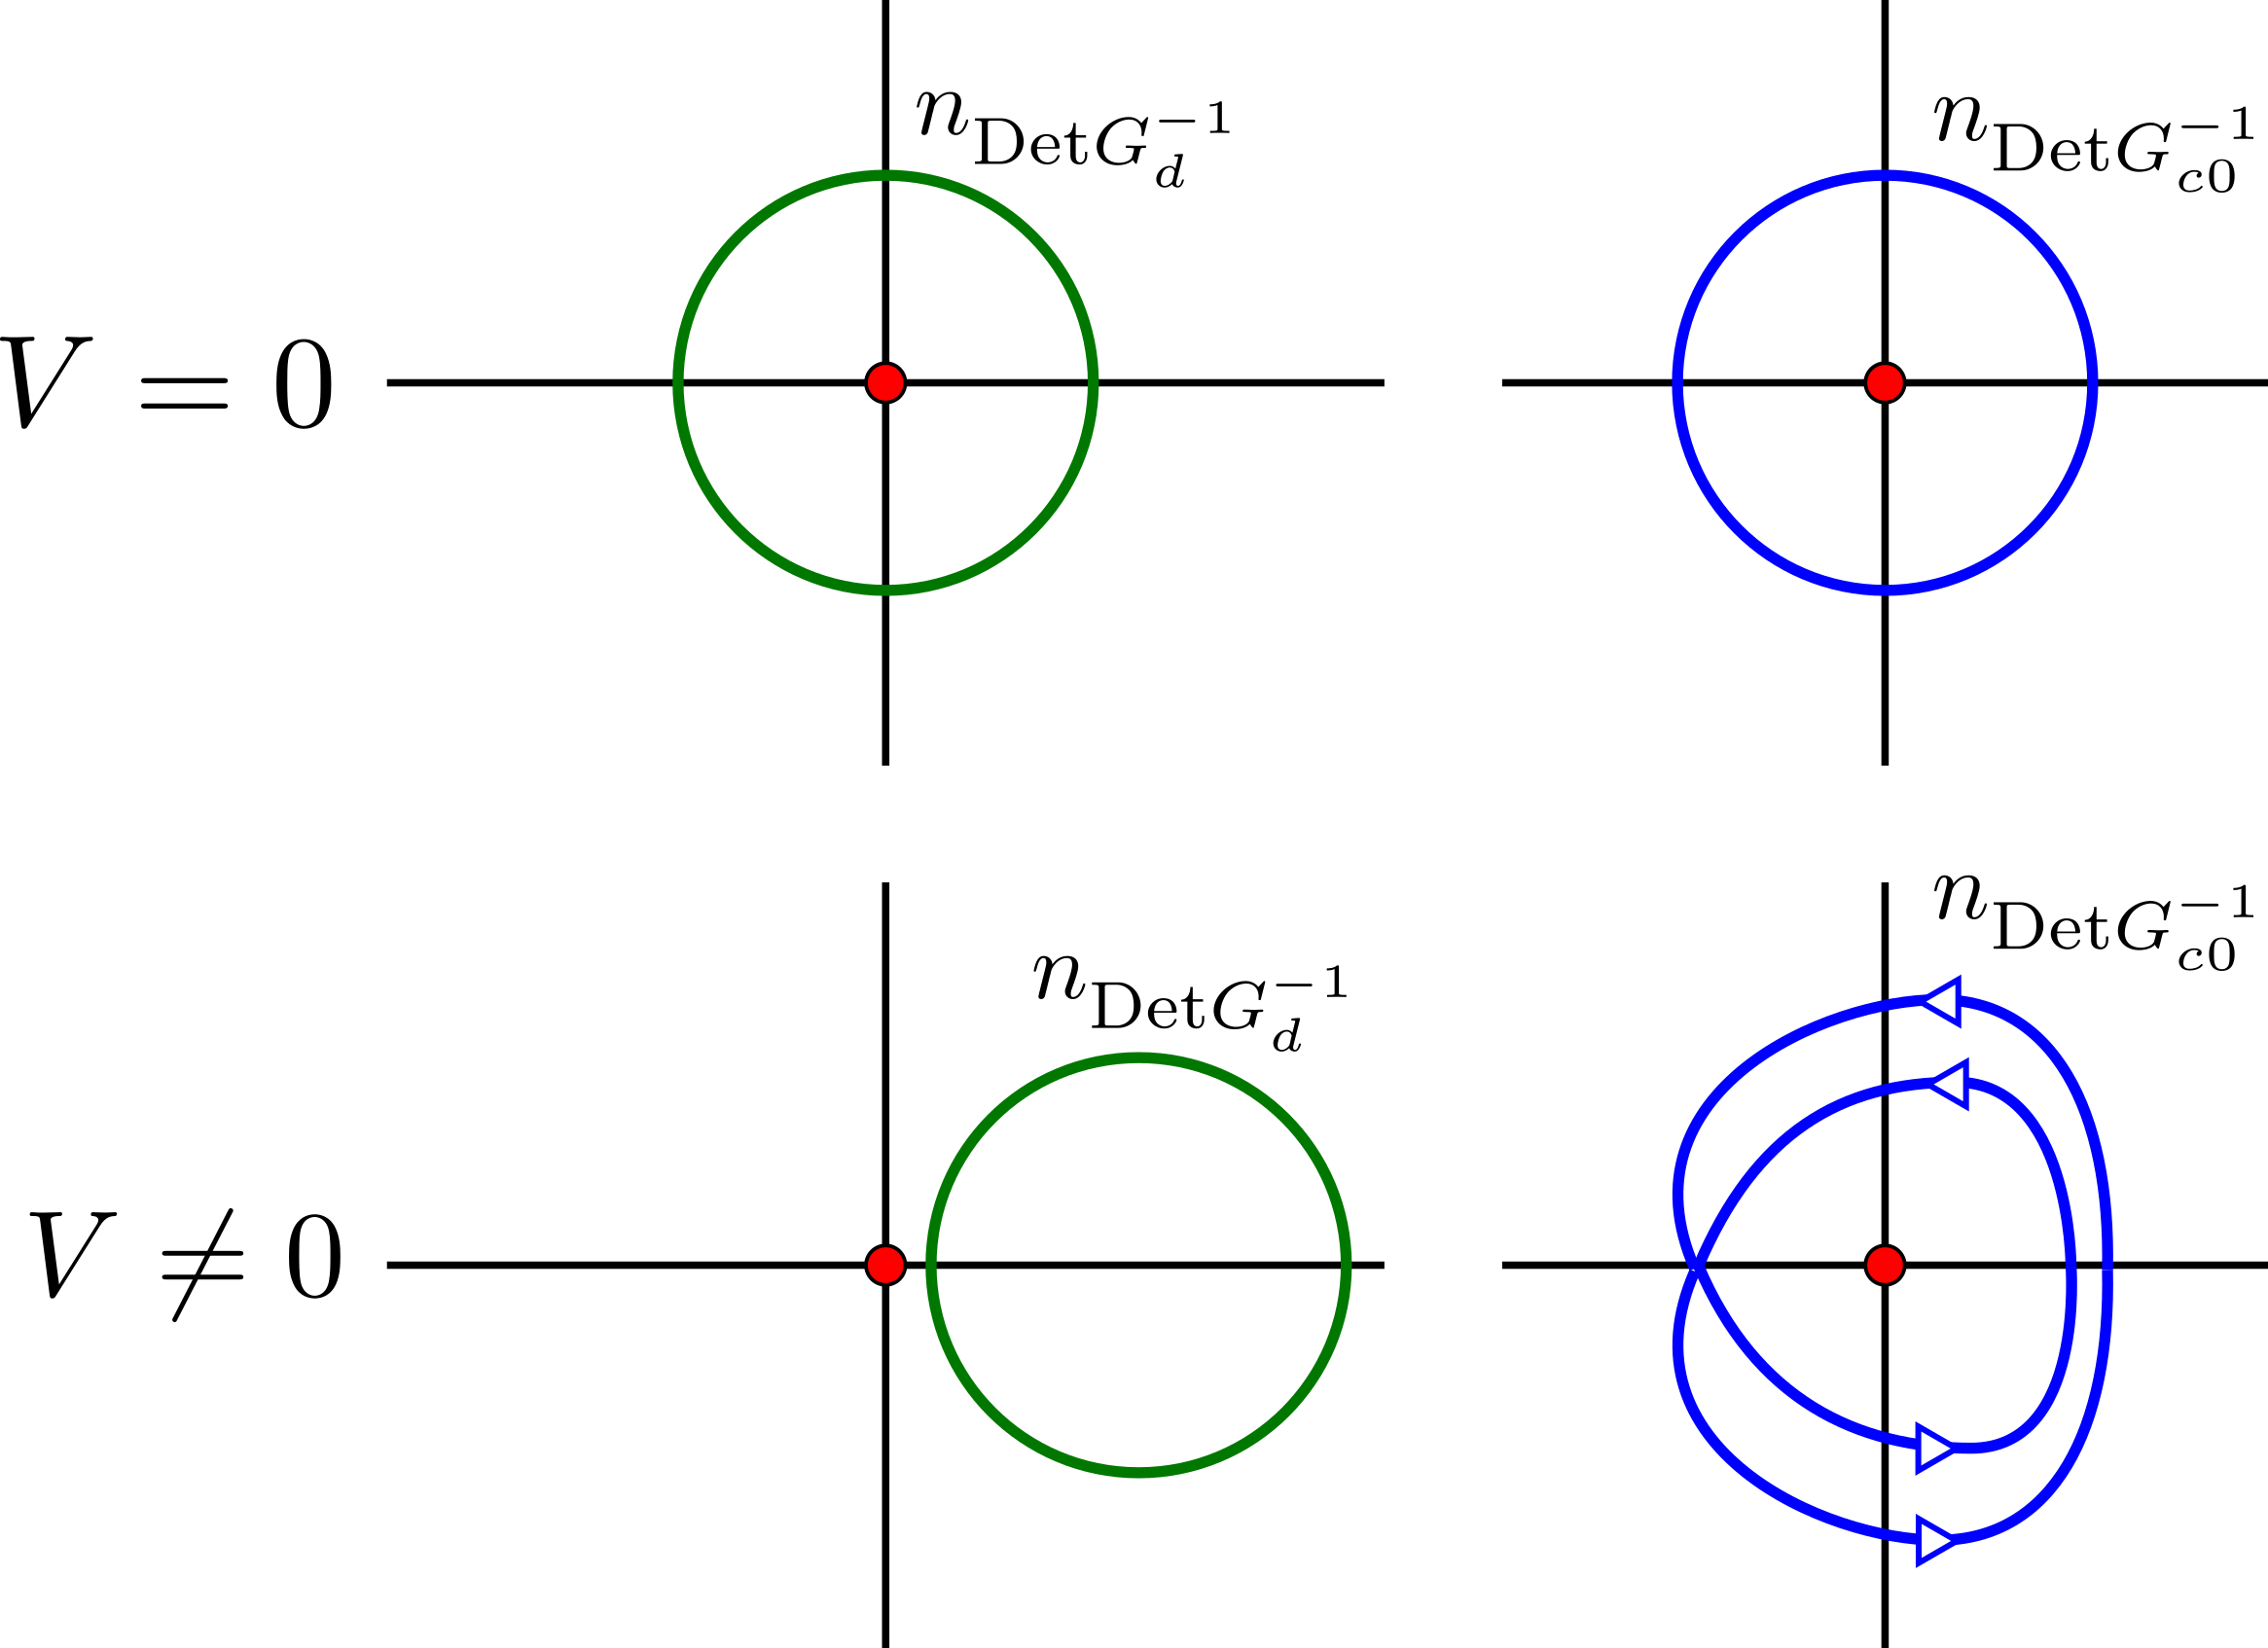
\includegraphics[scale=0.2]{../figures/luttinger_top_change.png}
\end{figure}
This is a specific case of the more general result for Kondo lattices obtained by Oshikawa using flux-insertion arguments in \cite{oshikawa2000topological}.
One can now ask what happens to this result once we also incorporate the spin-exchange interaction \(J \vec{S_d}\cdot\vec{s}\); we can expect that it will complicate the self-energy of the impurity. It cannot, however, preclude the loss of the real pole, nor can it create a new singularity - to do so would require the self-energy to diverge, and we are working with finite systems here. This suggests that the eq.~\eqref{luttinger_change} would still hold.

We have also not accounted for the RG flow from the local moment fixed point to the strong-coupling fixed point. The local moment fixed point is characterized by a decoupled quantum top:
\begin{equation}\begin{aligned}
	\mathcal{H}_\text{LM} = \epsilon_d \hat n_d + U \hat n_{d \uparrow} \hat n_{d \downarrow}
\end{aligned}\end{equation}
It can be shown that the single-particle Green's function for this effective Hamiltonian is similar to the one at the free-orbital fixed point. We will use the equation of motion technique to solve for the Green's function. The time-domain retarded Green's function is defined as
\begin{equation}\begin{aligned}
	G_{d\sigma}(t, t^\prime) = -i\theta(t-t^\prime) \left<\left\{ c_{d\sigma}(t), c^\dagger_{d\sigma}(t^\prime) \right\} \right>
\end{aligned}\end{equation}
Since the Hamiltonian is time-translation invariant, we can drop one of the instants:
\begin{equation}\begin{aligned}
	G_{d\sigma}(t, 0) = -i\theta(t) \left<\left\{ c_{d\sigma}(t), c^\dagger_{d\sigma}(0) \right\} \right>
\end{aligned}\end{equation}
The time derivative is
\begin{equation}\begin{aligned}
	\partial_t G_{d\sigma} &= -i \left[\partial_t \theta(t) \left<\left\{ c_{d\sigma}(t), c^\dagger_{d\sigma}(0) \right\} \right> + \theta(t) \partial_t \left<\left\{ c_{d\sigma}(t), c^\dagger_{d\sigma}(0) \right\} \right>\right] \\
			       &= -i \left[\delta(t) \left<\left\{ c_{d\sigma}(t), c^\dagger_{d\sigma}(0) \right\} \right> + \theta(t) \left<\left\{ \partial_t c_{d\sigma}(t), c^\dagger_{d\sigma}(0) \right\} \right>\right] = -i \delta(t) -i\theta(t) \left<\left\{ \partial_t c_{d\sigma}(t), c^\dagger_{d\sigma}(0) \right\} \right>
\end{aligned}\end{equation}
From the Heisenberg equations of motion, we get
\begin{equation}\begin{aligned}
	i \partial_t c_{d\sigma}(t) = \left[c_{d\sigma}(t), \mathcal{H}_{LM}(t)\right] = \left[\epsilon_d + U \hat n_{d\overline\sigma}(t)\right]c_{d\sigma}(t)
\end{aligned}\end{equation}
Substituting this into the time-derivative gives
\begin{equation}\begin{aligned}
	\partial_t G_{d\sigma} &= -i \delta(t) -i \theta(t) \left<\left\{ -i\left[\epsilon_d + U \hat n_{d\overline\sigma}(t)\right]c_{d\sigma}(t), c^\dagger_{d\sigma}(0) \right\} \right> = -i \delta(t) - i\epsilon_d G_{d\sigma} - U \theta(t) \left<\hat n_{d\overline\sigma}(t)\left\{c_{d\sigma}(t), c^\dagger_{d\sigma}(0) \right\} \right>\\
\end{aligned}\end{equation}
We define another Greens function
\begin{equation}\begin{aligned}
	G^\prime = -i \theta(t) \left<\hat n_{d\overline\sigma}(t)\left\{c_{d\sigma}(t), c^\dagger_{d\sigma}(0) \right\} \right>
\end{aligned}\end{equation}
which satisfies the equation of motion
\begin{equation}\begin{aligned}
	\partial_t G^\prime = -i \delta(t) -i\theta(t) \left<\left\{\partial_t \hat n_{d\overline\sigma}(t)c_{d\sigma}(t), c^\dagger_{d\sigma}(0) \right\} \right> -i\theta(t) \left<\left\{\hat n_{d\overline\sigma}(t)\partial_t c_{d\sigma}(t), c^\dagger_{d\sigma}(0) \right\} \right>
\end{aligned}\end{equation}
The second term vanishes because \(\left[\hat n_{d\overline\sigma}, \mathcal{H}_{LM}\right] = 0\) and hence \(\partial_t \hat n_{d\overline\sigma} = 0\). Also,
\begin{equation}\begin{aligned}
	\hat n_{d\overline\sigma}(t)\partial_t c_{d\sigma}(t) = -i\hat n_{d\overline\sigma}(t)\left[\epsilon_d + U \hat n_{d\overline\sigma}(t)\right]c_{d\sigma}(t) = -i\left[\epsilon_d + U\right]\hat n_{d\overline\sigma}(t)c_{d\sigma}(t)
\end{aligned}\end{equation}
Therefore,
\begin{equation}\begin{aligned}
	\partial_t G^\prime = -i \delta(t) \left< \hat n_{d\overline\sigma}(0)\right>- \left[\epsilon_d + U\right]\theta(t) \left<\left\{\hat n_{d\overline\sigma}(t)c_{d\sigma}(t), c^\dagger_{d\sigma}(0) \right\} \right> = -i \delta(t) -i \left( \epsilon_d + U \right) G^\prime
\end{aligned}\end{equation}
Changing all quantities to frequency-domain:
\begin{equation}\begin{aligned}
	G^\prime(t) &= \int_{-\infty}^\infty d\omega e^{-i\omega t} G^\prime(\omega)\\
	\partial_t G^\prime(t) &= -\int_{-\infty}^\infty d\omega i \omega e^{-i\omega t} G^\prime(\omega)\\
	\delta(t) &= \int_{-\infty}^\infty d\omega e^{-i\omega t}
\end{aligned}\end{equation}
Substituting these forms in the equation and comparing the coefficients of \(e^{i\omega t}\) gives
\begin{equation}\begin{aligned}
	 \omega G^\prime(\omega) =  \left< \hat n_{d\overline\sigma}(0)\right> + \left( \epsilon_d + U \right) G^\prime(\omega)\implies G^\prime(\omega) = \frac{\left< \hat n_{d\overline\sigma}(0)\right>}{\omega - \epsilon_d - U}
\end{aligned}\end{equation}
The equation of motion \(G_{d\sigma}\) can now be solved
\begin{equation}\begin{aligned}
	\partial_t G_{d\sigma}(t) &= -i \delta(t) - i\epsilon_d G_{d\sigma}(t) - iU G^\prime_{d\sigma}(t) \implies \omega G_{d\sigma}(\omega) = 1 + \epsilon_d G_{d\sigma}(\omega) + U\frac{\left< \hat n_{d\overline\sigma}(0)\right>}{\omega - \epsilon_d - U}\\
	\implies G_{d\sigma}(\omega) &= \frac{1}{\omega - \epsilon_d} + \frac{U\left< \hat n_{d\overline\sigma}(0)\right>}{\left( \omega - \epsilon_d \right) \left(\omega - \epsilon_d - U\right)}
\end{aligned}\end{equation}
For a particle-hole symmetric system, we can substitute \(\epsilon_d = -|\epsilon_d|\) and \(\epsilon_d + U = |\epsilon_d|\).
\begin{equation}\begin{aligned}
	G_{d\sigma}(\omega) &= \frac{1}{\omega + |\epsilon_d|} + \frac{U\left< \hat n_{d\overline\sigma}(0)\right>}{\left( \omega + |\epsilon_d| \right) \left(\omega - |\epsilon_d|\right)}
\end{aligned}\end{equation}
which reveals two poles at \(\pm |\epsilon_d|\), one above and one below the Fermi surface. Since the RHS of eq.~\eqref{total_lutt} counts the number of poles on or below the FS, we will still count one pole for \(G_{d\sigma}\). Thus, this Green's function is topological similar to the free-orbital one at \(T=0\).

The scattering phase shift suffered by the conduction electrons at the Fermi surface, off the impurity, can be calculated from the impurity occupancy, using the Friedel sum rule. From the ground state wavefunction, we can calculate the average number of particles on the impurity:
\begin{equation}\begin{aligned}
	\left<n_d \right> = \bra{\Psi}_1\sum_\sigma \hat n_{d\sigma} \ket{\Psi}_1
\end{aligned}\end{equation}
\(\ket{\Psi}_1\) is the lower energy state in eq.~\eqref{gstate}. Performing the inner product gives
\begin{equation}\begin{aligned}
	\left<n_d \right> = \left( c_s^- \right)^2 + \left( c_c^- \right)^2 = 1
\end{aligned}\end{equation}
The phase shift is thus
\begin{equation}\begin{aligned}
	\frac{1}{\pi}\sum_\sigma \delta_\sigma(0) = \left<n_d \right> \implies \delta_\sigma(0) = \frac{\pi}{2}
\end{aligned}\end{equation}
There we used \(\delta_\uparrow = \delta_\downarrow\) because the model is SU(2)-symmetric. This line of arguments was first presented for the Kondo model in \cite{martin_prl_1982}.

The change in Luttinger's number also allows us to calculate the Wilson ratio of the system, from eq.~\eqref{wilson_luttinger}.
\begin{equation}\begin{aligned}
	R = 1 + \sin^2 \left( \frac{\pi}{2}\Delta N_L \right) = 1 + \sin^2 \frac{\pi}{2} = 2
\end{aligned}\end{equation}
\section{Reverse RG analysis}\label{rev_rg}
The goal here is to chart the journey starting from the IR fixed point towards the UV regime, by following one particular wavefunction. We will start with a very simple IR ground state wavefunction, and then go back towards the UV ground state by applying the inverse unitary operator \(U^\dagger\):
\begin{equation*}\begin{aligned}
	U : \underbrace{\ket{1,2,...,N}}_\text{UV ground state} \rightarrow \ket{1,2,...,N-1}\ket{N} \rightarrow ... \rightarrow \underbrace{\ket{1,2,...,N^*}\ket{N^*+1}...\ket{N}}_\text{IR ground state}
\end{aligned}\end{equation*}
\begin{equation*}\begin{aligned}
	U^\dagger : \underbrace{\ket{1,2,...,N^*}\ket{N^*+1}...\ket{N}}_\text{IR ground state} \rightarrow \ket{1,2,...,N^*+1}\ket{N^*+2}...\ket{N} \rightarrow ... \rightarrow\underbrace{\ket{1,,2,...,N}}_\text{UV ground state}
\end{aligned}\end{equation*}
The first process is the forward RG which we used to obtain the scaling equations. The second process is the reverse RG which we will undertake now. In general, we start with an IR wavefunction that consists a certain number of momentum states \(n_1\) still entangled with the impurity, and the remaining momentum states \(n_2\) disentangled from the impurity. The former are said to be part of the emergent Kondo cloud, while the latter are said to be part of the integrals of motion (IOMs) and appear in direct product with the cloud+impurity system in the ground state wavefunction. Each momentum state is tagged with two conduction bath levels, one above the Fermi surface and one below. These will be represented as \(k,\pm\). If we represent the emergent cloud momentum states as \(\left\{k_i\right\} \) and the IOM states as \(\left\{q_i\right\}\), the ground state wavefunction can be written as 
\begin{equation}\begin{aligned}
	\ket{\Psi}_0 = \left(\otimes_{i=1}^{n_2}\ket{q_i,-,\uparrow}\ket{q_i,-,\downarrow}\right)\ket{\Phi}_\text{cloud}\left(\otimes_{i=1}^{n_2}\ket{q_i,+,\uparrow}\ket{q_i,+,\downarrow}\right)
\end{aligned}\end{equation}
Throughout, we have assumed that the IOMs below the Fermi surface are occupied while those above are unoccupied. This means:
\begin{equation}\begin{aligned}
	\ket{\Psi}_0 = \left(\otimes_{i=1}^{n_2}\ket{\hat n_{q_i,-,\uparrow}=1}\ket{\hat n_{q_i,-,\downarrow}=1}\right)\ket{\Phi}_\text{cloud}\left(\otimes_{i=1}^{n_2}\ket{\hat n_{q_i,+,\uparrow}=0}\ket{\hat n_{q_i,+,\downarrow}=0}\right)
\end{aligned}\end{equation}
\(\ket{\Phi}_\text{cloud}\) will be obtained by diagonalising a small system of \(n_1\) conduction bath \(k\) states. This completes the construction of the IR ground state \(\ket{\Psi}_0\). The algorithm of reverse RG then involves applying unitary transformations on this IR wavefunction; the unitary transformations will be the inverse of those that were applied during the forward RG algorithm. Since the forwards RG transformations decoupled \(k\) states and transformed them into the IOMS, the inverse transformations will take the momentum states in the IOMs and re-entangle them with the impurity+cloud system, one at a time. This is shown in fig.~\ref{rev-rg}.
\begin{figure}[!htbp]
	\centering
	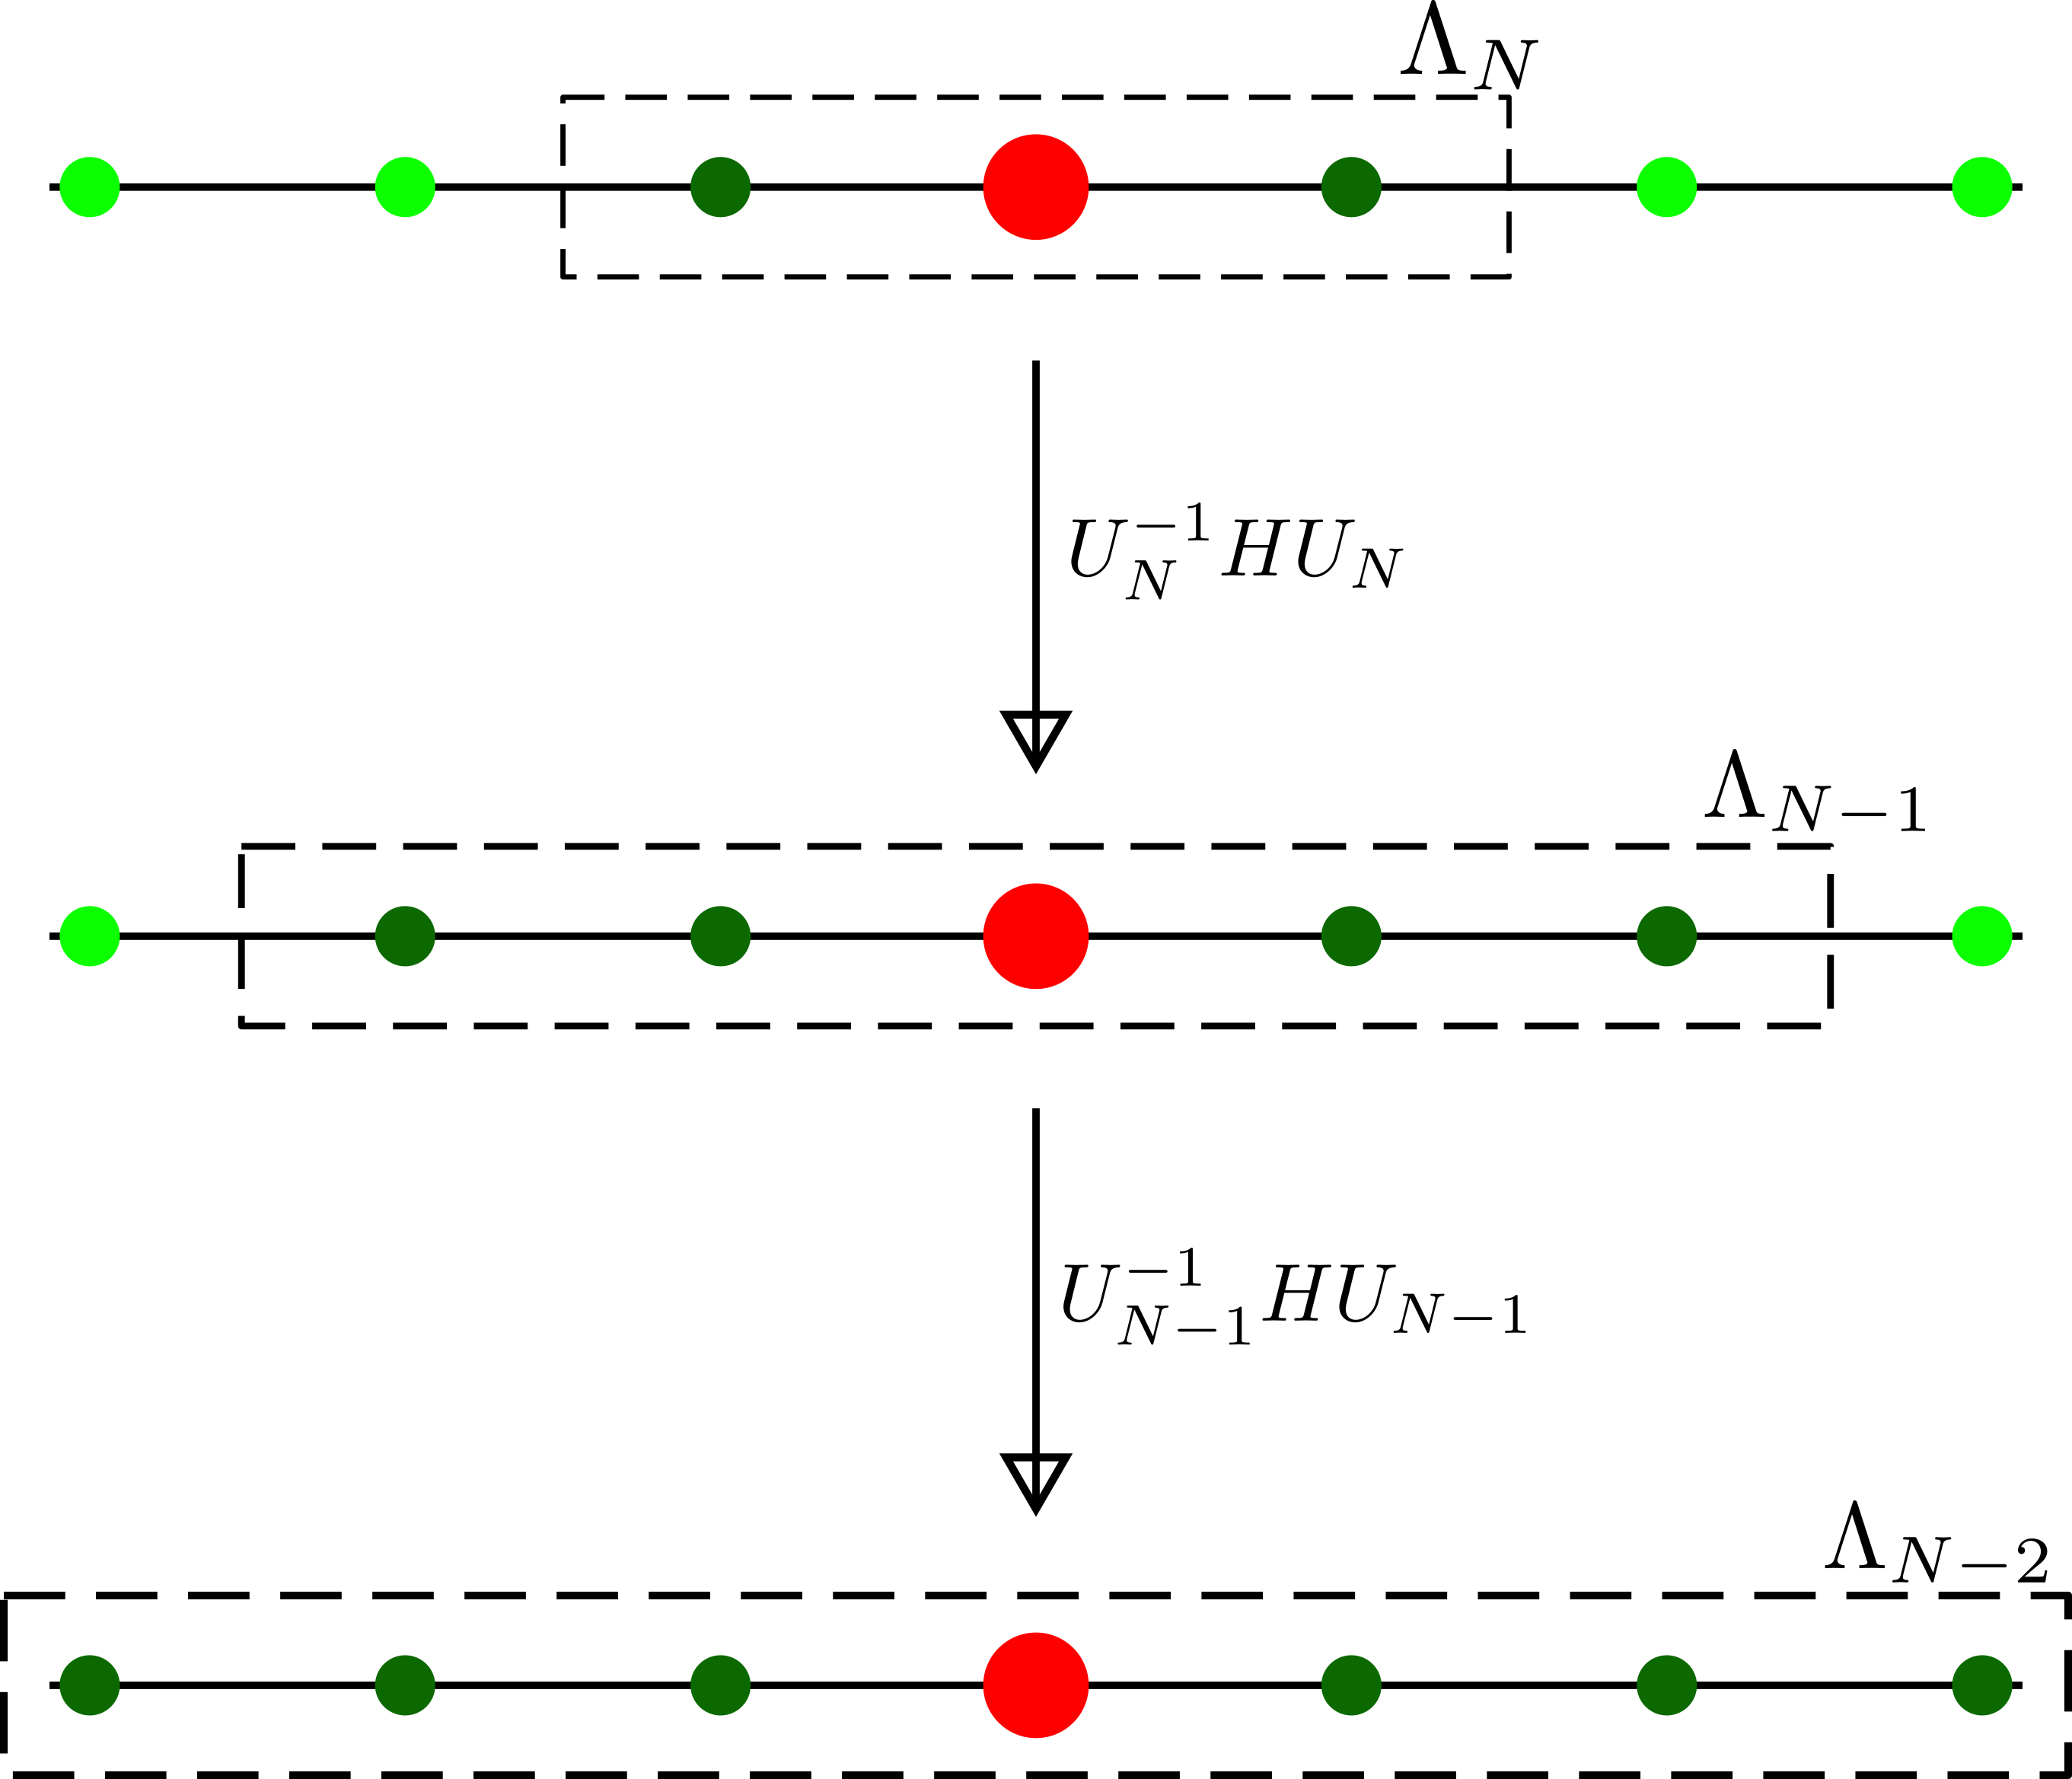
\includegraphics[width=0.4\textwidth]{../figures/reverse-rg.png}
	\caption{We start with a Hamiltonian with an impurity site (red) coupled with two conduction electrons (dark green), with four other decoupled electrons (bright green). The dotted rectangle represents the emergent window \(\left( -\Lambda_j, \Lambda_j \right) \) at each step; the electrons inside that rectangle are still entangled with the impurity, while the ones inside have been decoupled. The next step of reverse RG involves applying the inverse transformation on the Hamiltonian, which will couple two more electrons from the IOMS (hence four dark green circles in the second step), leading to an enlargement of the emergent window. The unitary varies for each step, hence the notation \(U_j\).}
	\label{rev-rg}
\end{figure}

The next step is to write down the unitaries that will take us from the IR ground state to the UV ground state. In the forward RG, we used the following unitary for decoupling the shell \(\epsilon_q\) and spin \(\beta\) is
\begin{equation}\begin{aligned}
	U_{q\beta} = \frac{1}{\sqrt 2}\left[1 + \eta_{0 \beta} + \eta_{1\beta}^\dagger\right]~.
\end{aligned}\end{equation}
Here, the subscripts \(0\) and \(1\) indicate it decouples an electron above and below the Fermi surface respectively. The inverse transformation for re-entangling \(q\beta\) is
\begin{equation}\begin{aligned}
	U^\dagger_{q\beta} = \frac{1}{\sqrt 2}\left[1 + \eta_{0 \beta}^\dagger + \eta_{1\beta}\right]~.
\end{aligned}\end{equation}
In the \(U>0\) regime, the \(\eta\)s are given by
\begin{equation}\begin{aligned}
	\eta_{0\beta}^\dagger = V \left[\frac{1}{d_0}\left( 1 - \hat n_{d\overline\beta} \right) + \frac{1}{d_1}\hat n_{d\overline\beta}  \right]c^\dagger_{q\beta}c_{d\beta} + \frac{1}{d_2}\frac{J}{2}\sum_{k} \left( S_d^z \beta c^\dagger_{q\beta}c_{k\beta} + c^\dagger_{d\overline\beta}c_{d\beta}c^\dagger_{q\beta}c_{k\overline\beta}\right) ~,\\
	\eta_{1\beta} = V \left[\frac{1}{d_1}\left( 1 - \hat n_{d\overline\beta} \right) + \frac{1}{d_0}\hat n_{d\overline\beta}  \right]c^\dagger_{d\beta}c_{q\beta} + \frac{1}{d_2}\frac{J}{2}\sum_{k} \left( S_d^z \beta c^\dagger_{k\beta}c_{q\beta} + c^\dagger_{d\beta}c_{d\overline\beta}c^\dagger_{k\overline\beta}c_{q\beta}\right)~;
\end{aligned}\end{equation}
since \(K\) is irrelevant, we have set \(K=0\) here. The denominators have already been defined in eq.~\eqref{denominators}.
\begin{equation}\begin{aligned}
	d_0 = \omega - \frac{D}{2} - \frac{U}{2} + \frac{K}{4}, \quad d_1 = \omega - \frac{D}{2} + \frac{U}{2} + \frac{J}{4}, \quad d_2 = \omega - \frac{D}{2} + \frac{J}{4}, \quad d_3 = \omega - \frac{D}{2} + \frac{K}{4}
\end{aligned}\end{equation}

The wavefunction after reversing one step of the RG will thus be
\begin{equation}\begin{aligned}
	\ket{\Psi}_1 = U^\dagger_{q \uparrow}U^\dagger_{q \downarrow}\ket{\Psi}_0
\end{aligned}\end{equation}
Here, \(q\) is the first momentum state immediately outside the emergent cloud. Re-entangling further momentum states using their respective unitaries lead to the sequence of wavefunctions \(\ket{\Psi}_2, \ket{\Psi}_3\) and so on.

\begin{figure}[!htbp]
	\centering
	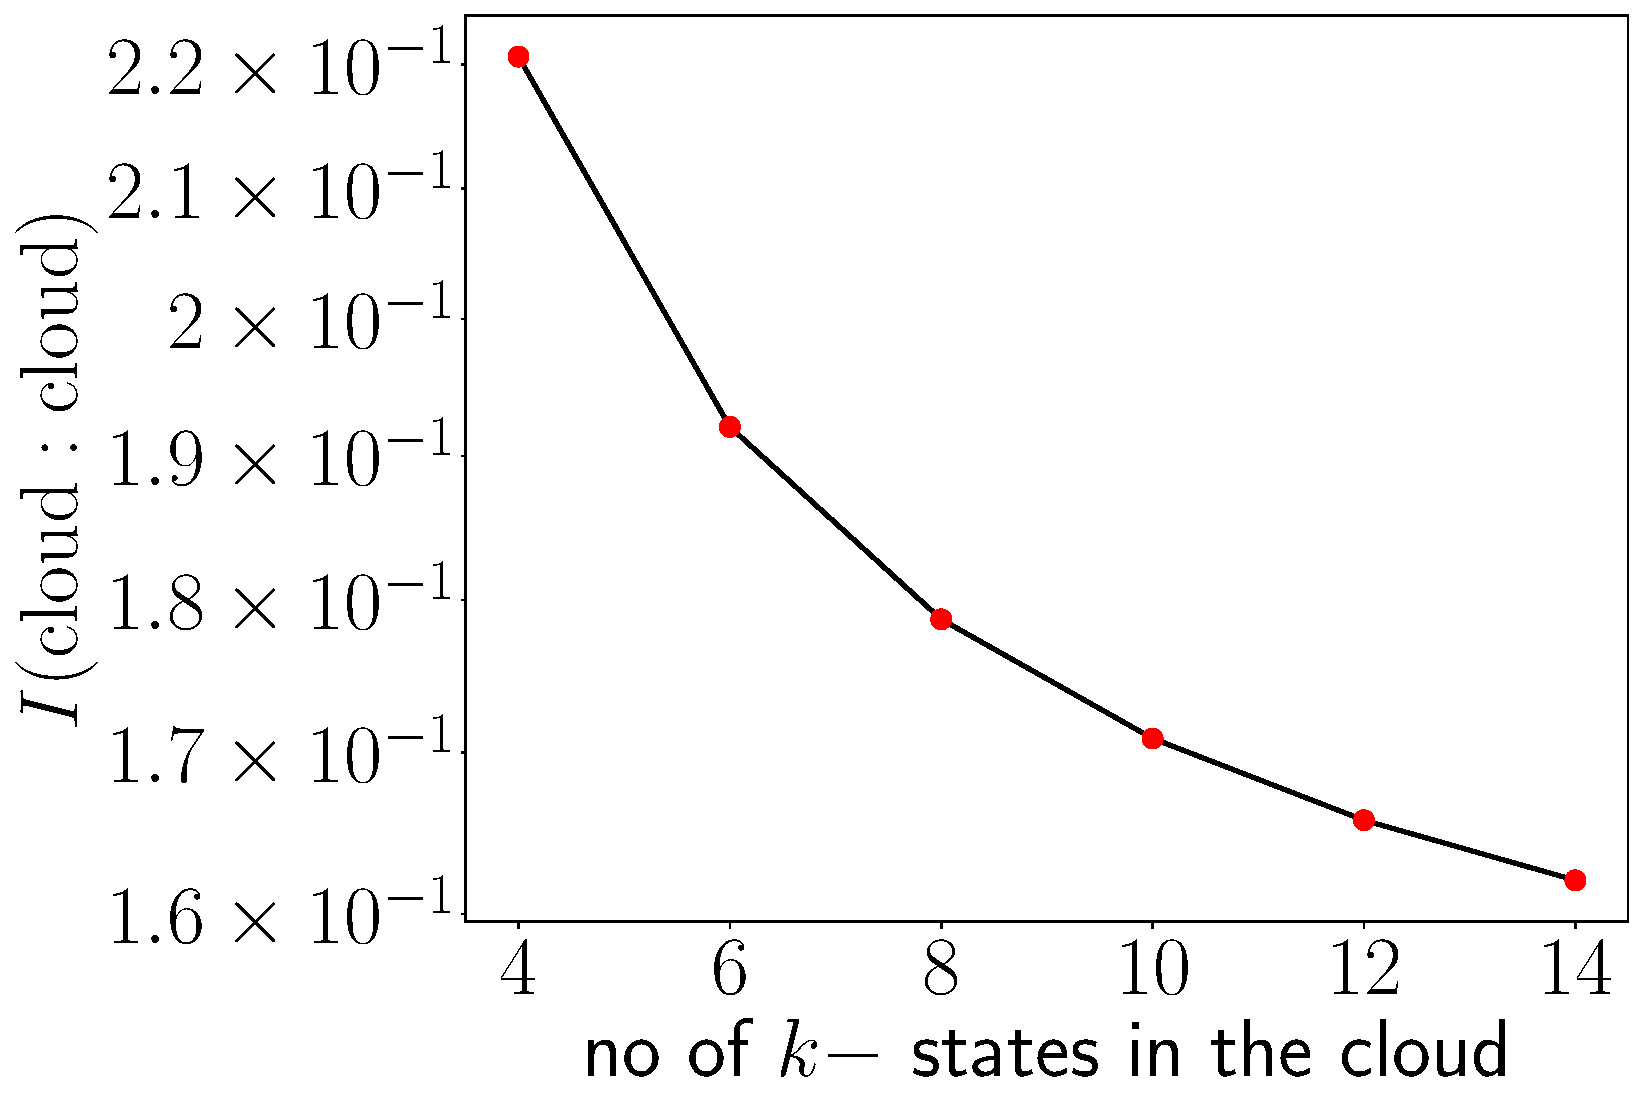
\includegraphics[width=0.45\textwidth]{../figures/mut_I_ee.pdf}
	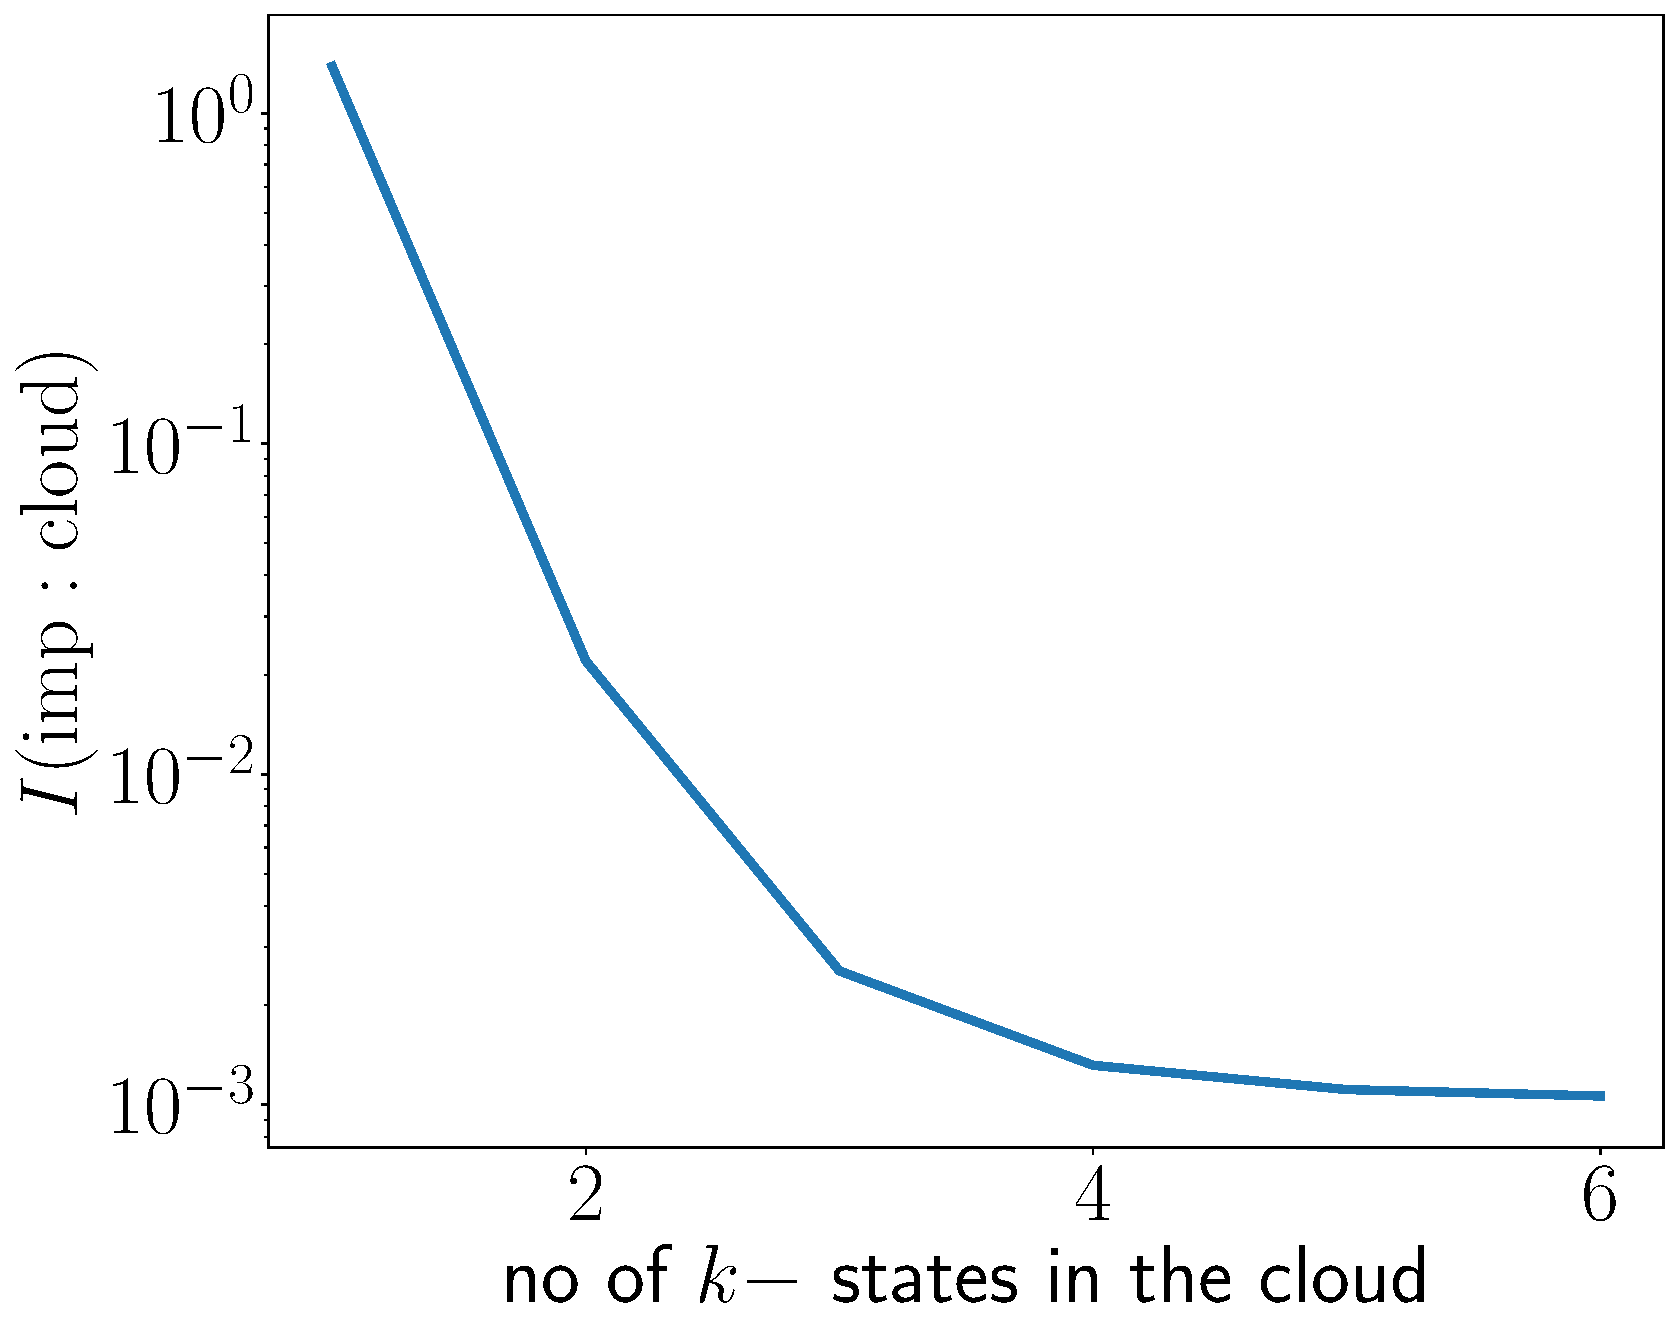
\includegraphics[width=0.45\textwidth]{../figures/mut_I_ie.pdf}
	\caption{\textit{Left}: Mutual information between two conduction electrons inside the cloud. \textit{Right}: Mutual information between a conduction electron inside the cloud and an impurity electron. Both the measures increase towards the strong-coupling fixed point, because of the distillation of the Kondo cloud brought about by the RG flow.}
	\label{mutI}
\end{figure}

\begin{figure}[!htbp]
	\centering
	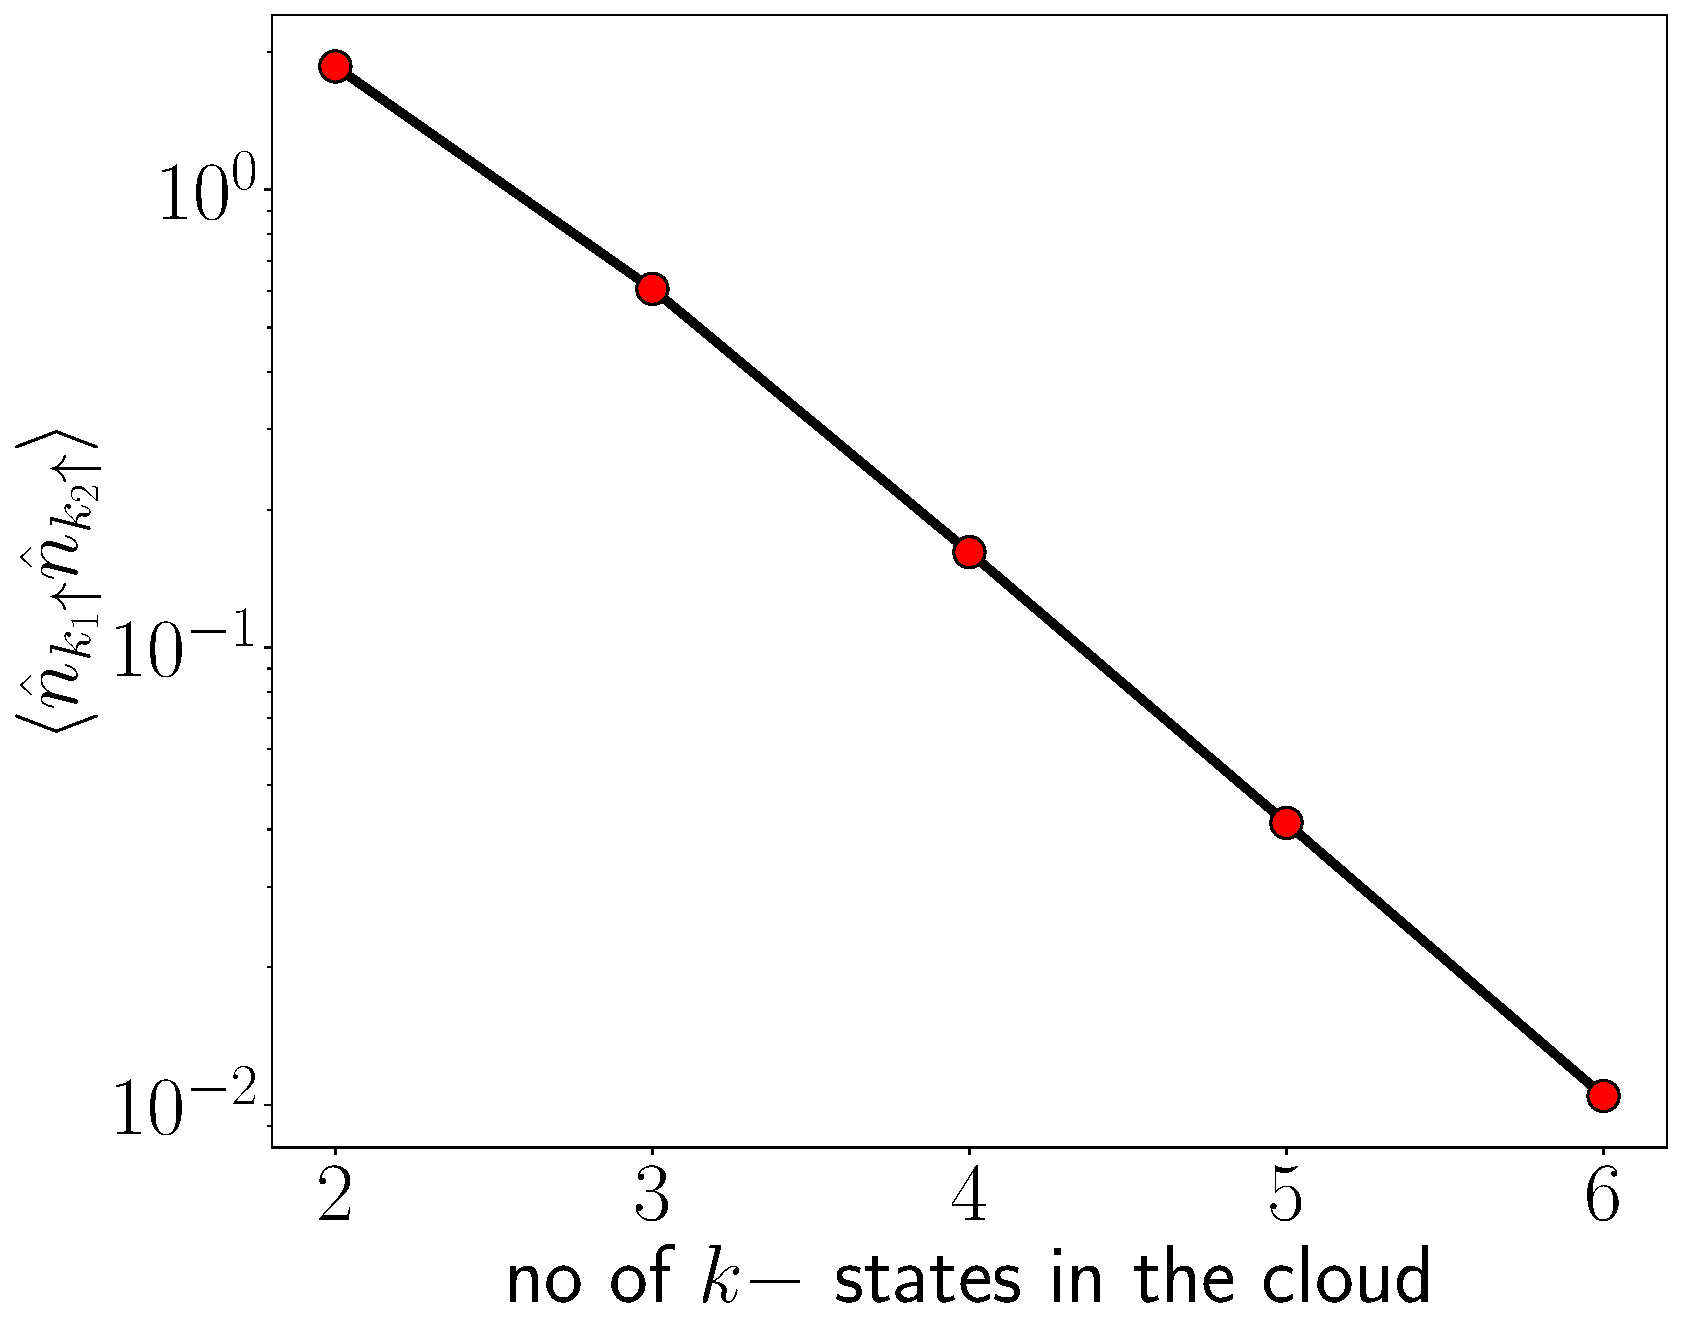
\includegraphics[width=0.45\textwidth]{../figures/corr_same.pdf}
	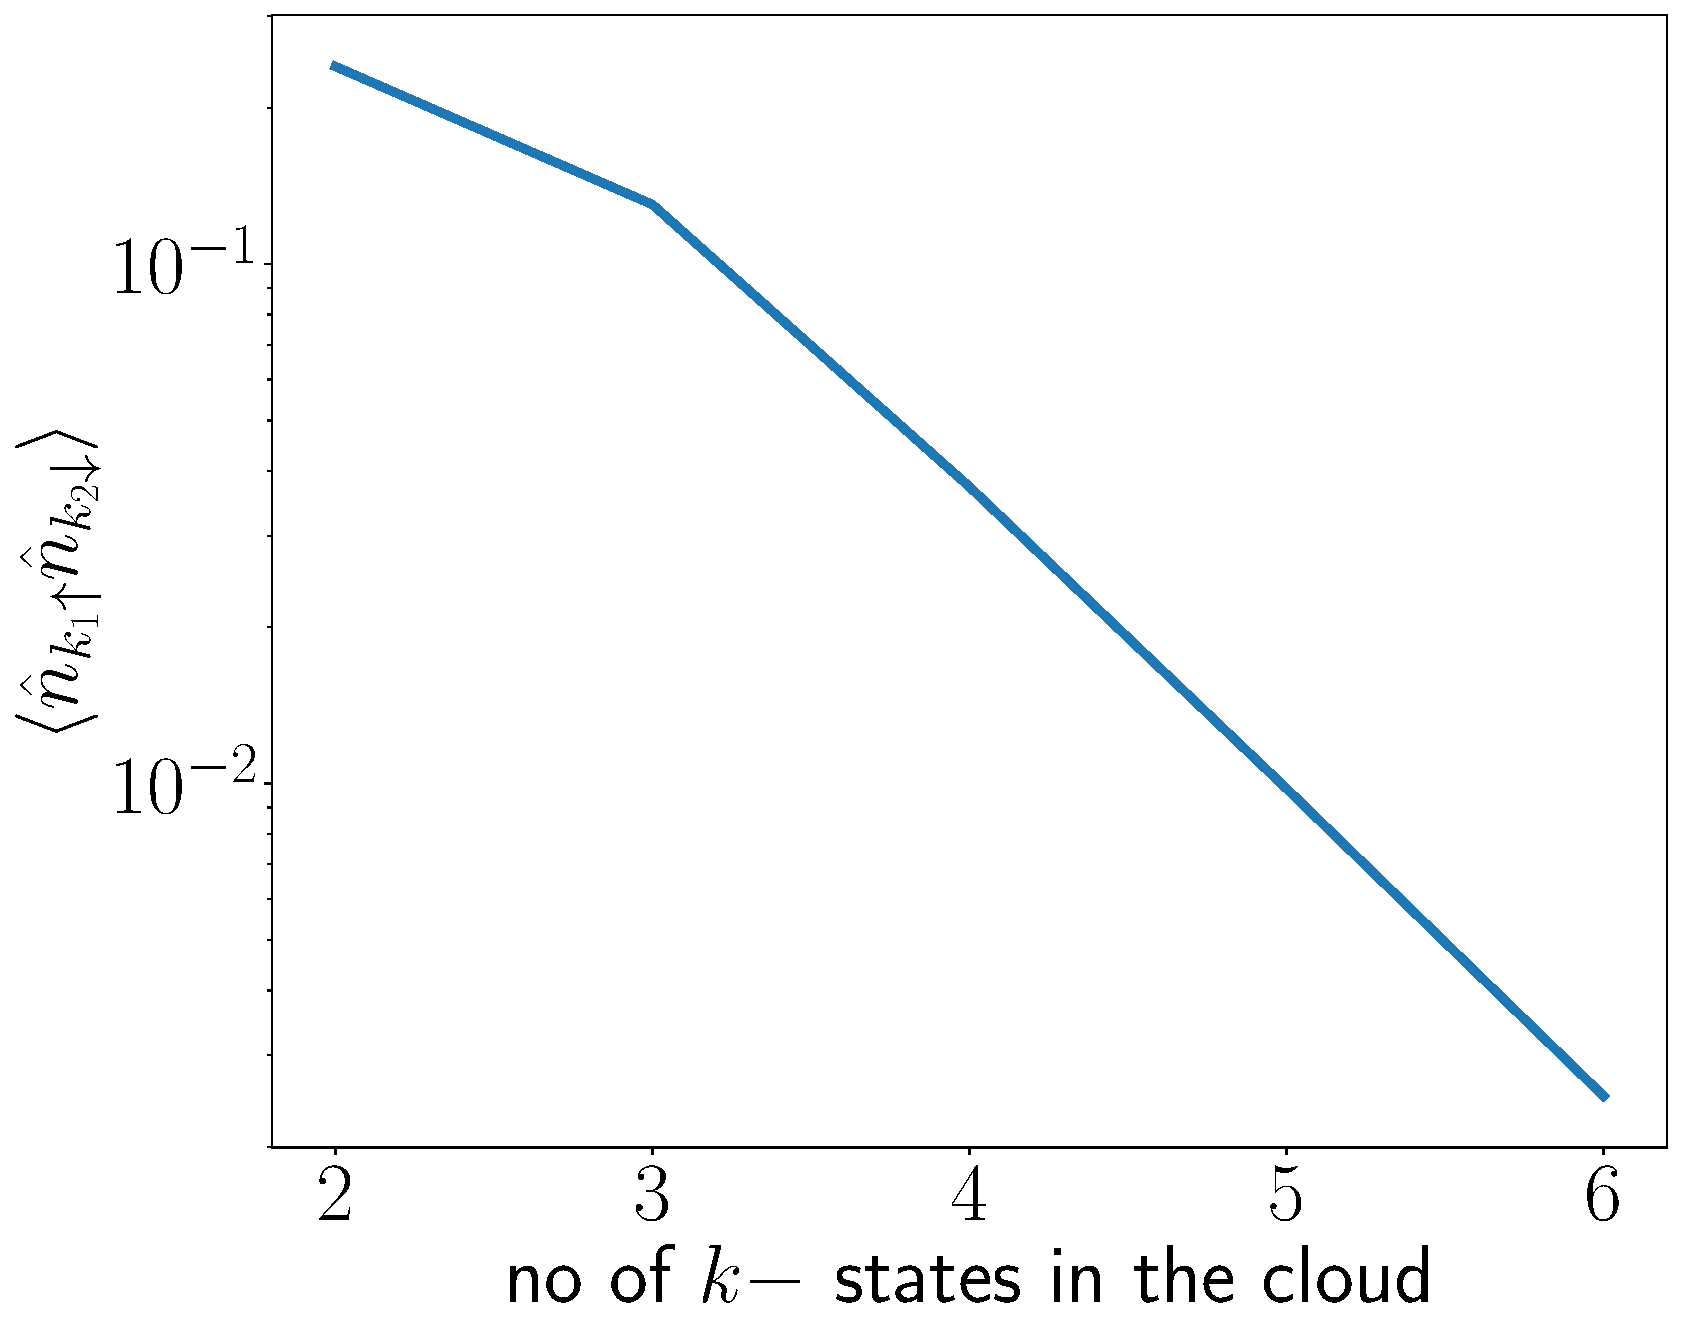
\includegraphics[width=0.45\textwidth]{../figures/corr_opp.pdf}
	\caption{Increase in the diagonal correlation functions between cloud electrons under RG flow towards the strong-coupling fixed point. This is consistent with the Fermi liquid pieces generated in the \(k-\)space effective Hamiltonian of the Kondo cloud.}
\end{figure}

\begin{figure}[!htbp]
	\centering
	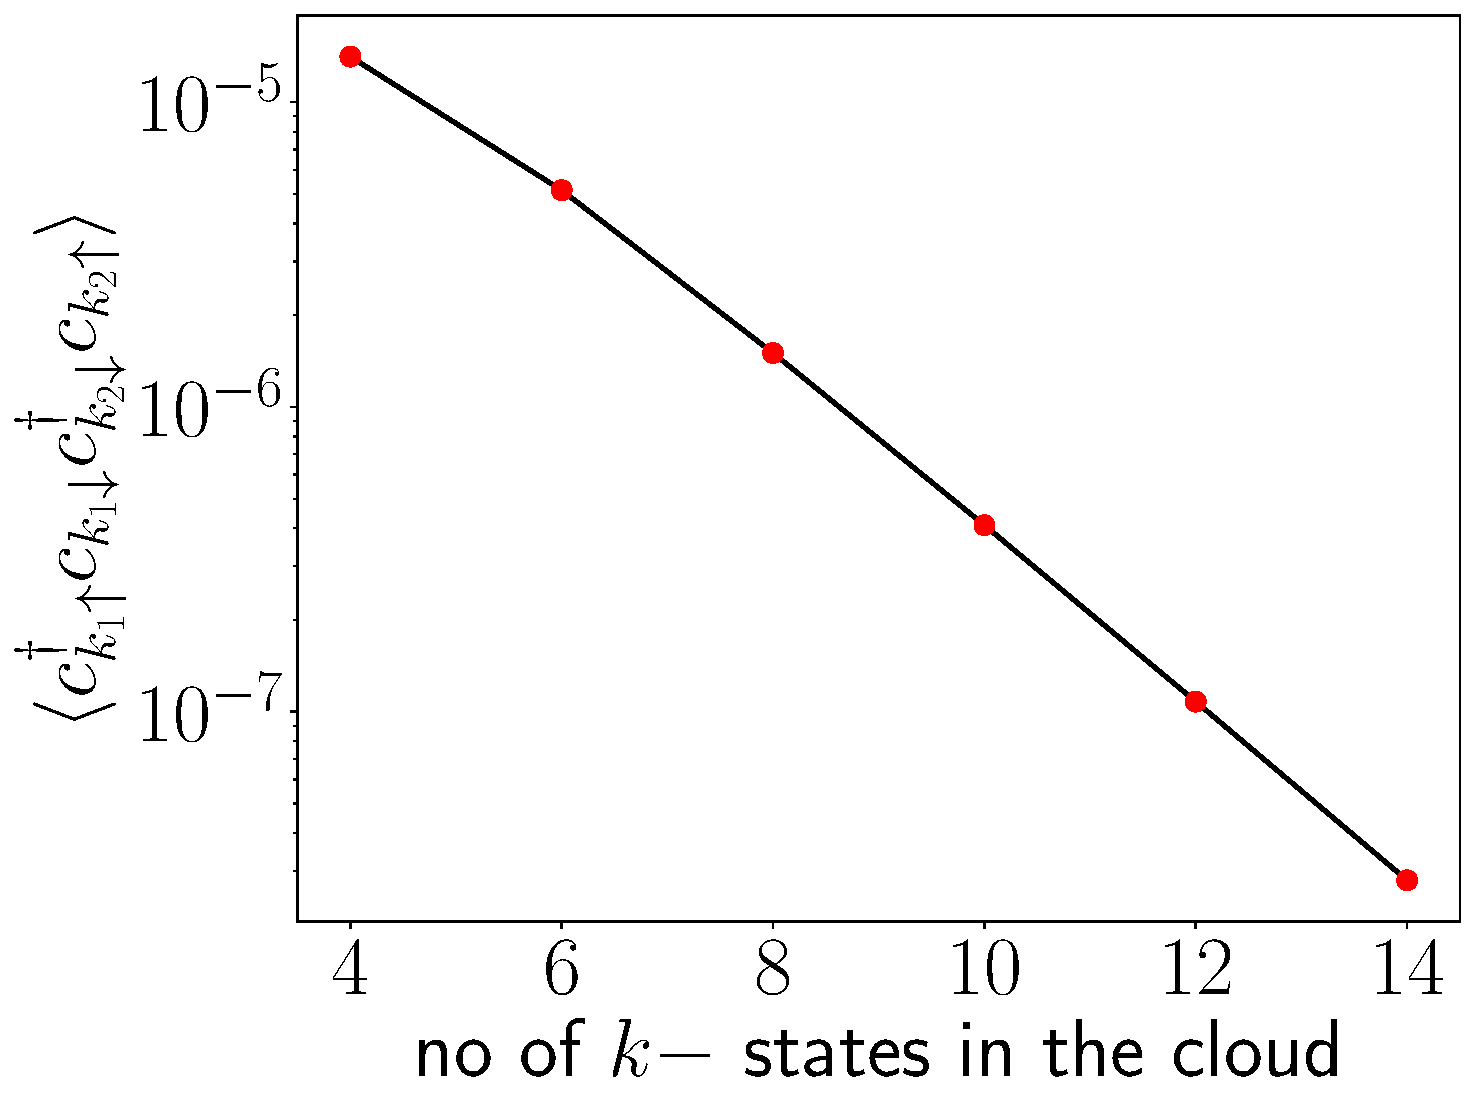
\includegraphics[width=0.45\textwidth]{../figures/corr_od.pdf}
	\caption{Growth of the off-diagonal correlation function between Kondo cloud electrons towards the strong-coupling fixed point. This is the direct cause of the screening of the impurity spin, and is a reflection of the off-diagonal two-particle scattering terms in the \(k-\)space effective Hamiltonian of the Kondo cloud.}
\end{figure}

The results of the reverse RG study are depicted in the following plots. We have used two types of quantities in the process - mutual information and correlation functions. The mutual information between two subsystems \(A\) and \(B\) in a wavefunction with many subsystems is defined as
\begin{equation}\begin{aligned}
	I(A: B) = S_A + S_B - S_{AB}
\end{aligned}\end{equation}
where \(S_{ij..q}\) is the von-Neumann entropy of the reduced density matrix obtained after tracing out all degrees of freedom except those in the subscript of \(S\).

The mutual information between two electrons inside the entangled cloud increases as we go towards the IR fixed point. This can be understood in the following manner; as the wavefunction flows towards a smaller sized emergent cloud, the entanglement between those electrons gets distilled out.

We have also computed some correlation functions. All of them increase towards the IR fixed point. The increase in the correlation function \(\left<\hat n_{k_1 \uparrow} \hat n_{k_2 \downarrow} \right>\) arises from the crystallization of the spin singlet at the fixed point. The increase in the correlation function \(\left<\hat n_{k \uparrow} \hat n_{k \downarrow} \right>\) arises from the charge triplet content of the wavefunction, showing the increase of the charge contribution on the momenta. The increase in the off-diagonal correlation function \(\left< c^\dagger_{k \uparrow}c_{k^\prime \downarrow}c^\dagger_{q \downarrow}c_{q^\prime \uparrow}\right>\) shows that the there is a large and non-trivial interaction between the electrons of the cloud that is being mediated by the impurity electron. This interaction is not of the Fermi liquid type, but instead was obtained in the effective Hamiltonian for the Kondo cloud.
